\chapter{Analysis Strategy}
\label{ch:analysis}

The \EWWZ process exhibits a distinct experimental signature characterized by two forward, 
high-momentum jets, typically arising from the hadronization of 
two valence quarks from each of the colliding
protons scattered away from the beam line, in addition 
to the vector bosons. We exploit the leptonic decay channel of the $\PW$ and $\PZ$
bosons in this analysis, as the three-lepton event signature is relatively free
from other background processes. 
Events with exactly three leptons (electrons or muons), 
missing transverse momentum, 
and two jets at high pseudorapidity $\eta$ with large dijet system invariant mass {\mjj}
are selected for this analysis.
A candidate \EWWZ event selected by this analysis,
demonstrating these characteristics, is shown in Fig.~\ref{fig:eventView}.

\begin{figure}[htbp]
  \centering
   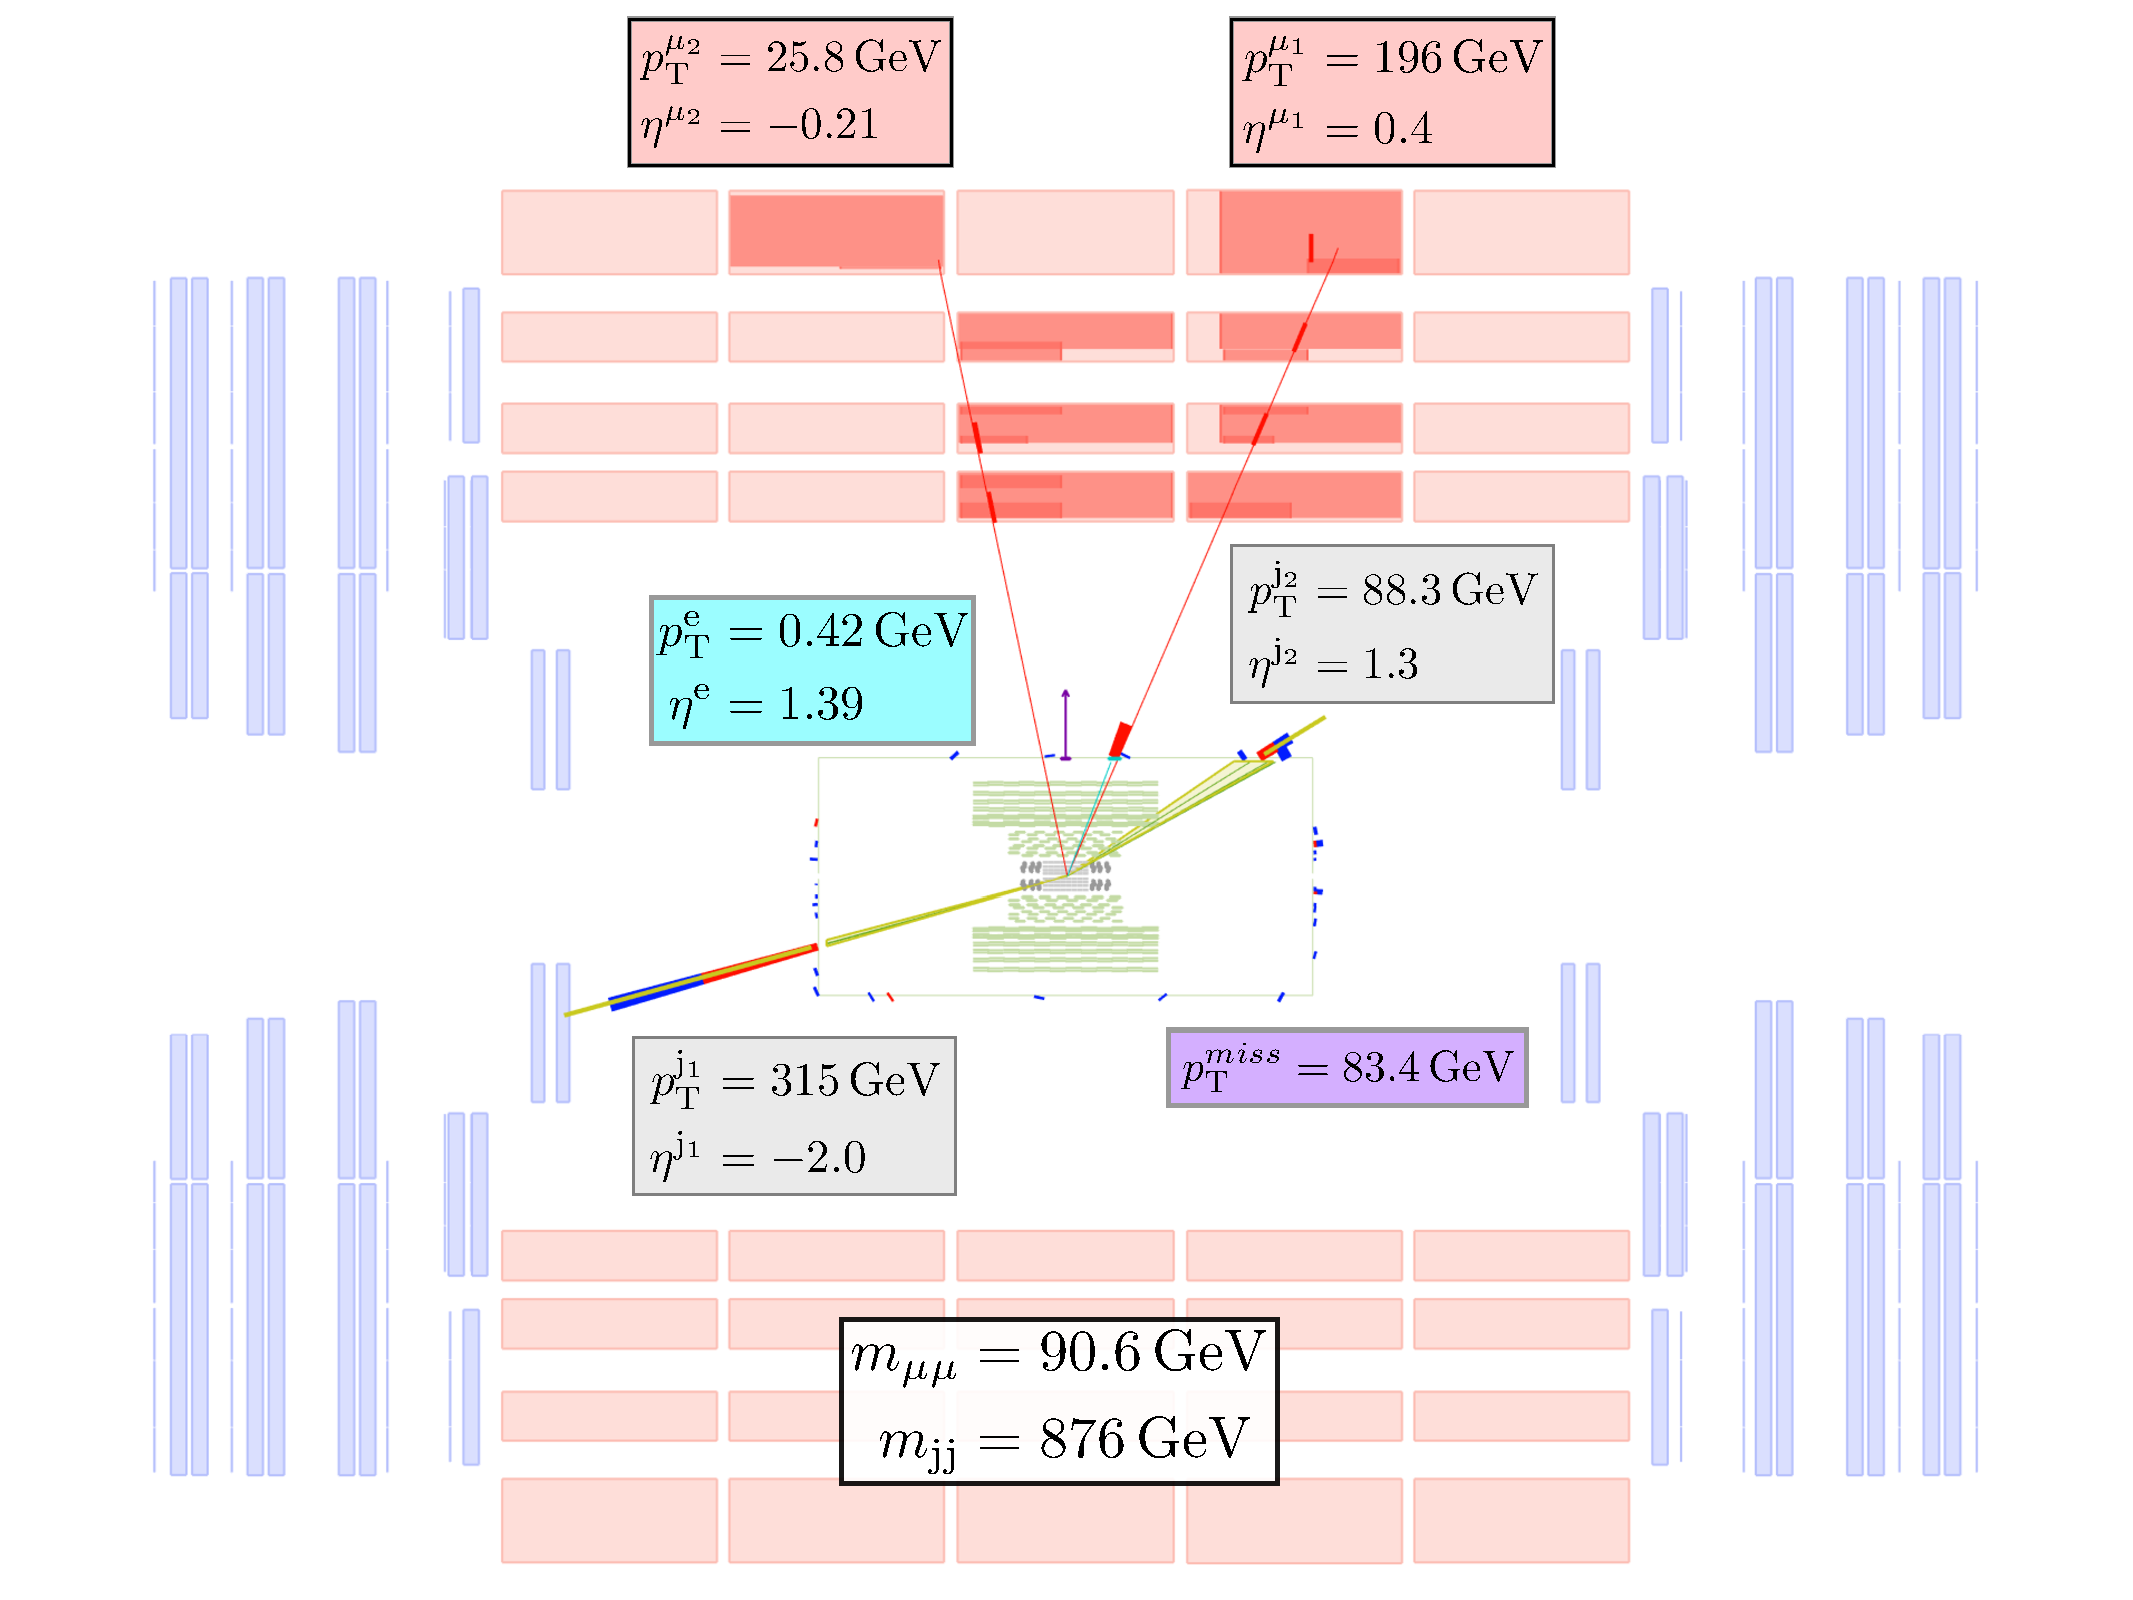
\includegraphics[width=0.6\textwidth]{figures/AnalysisProcedure/AnnotatedEventViewWZjjZProj.pdf}
   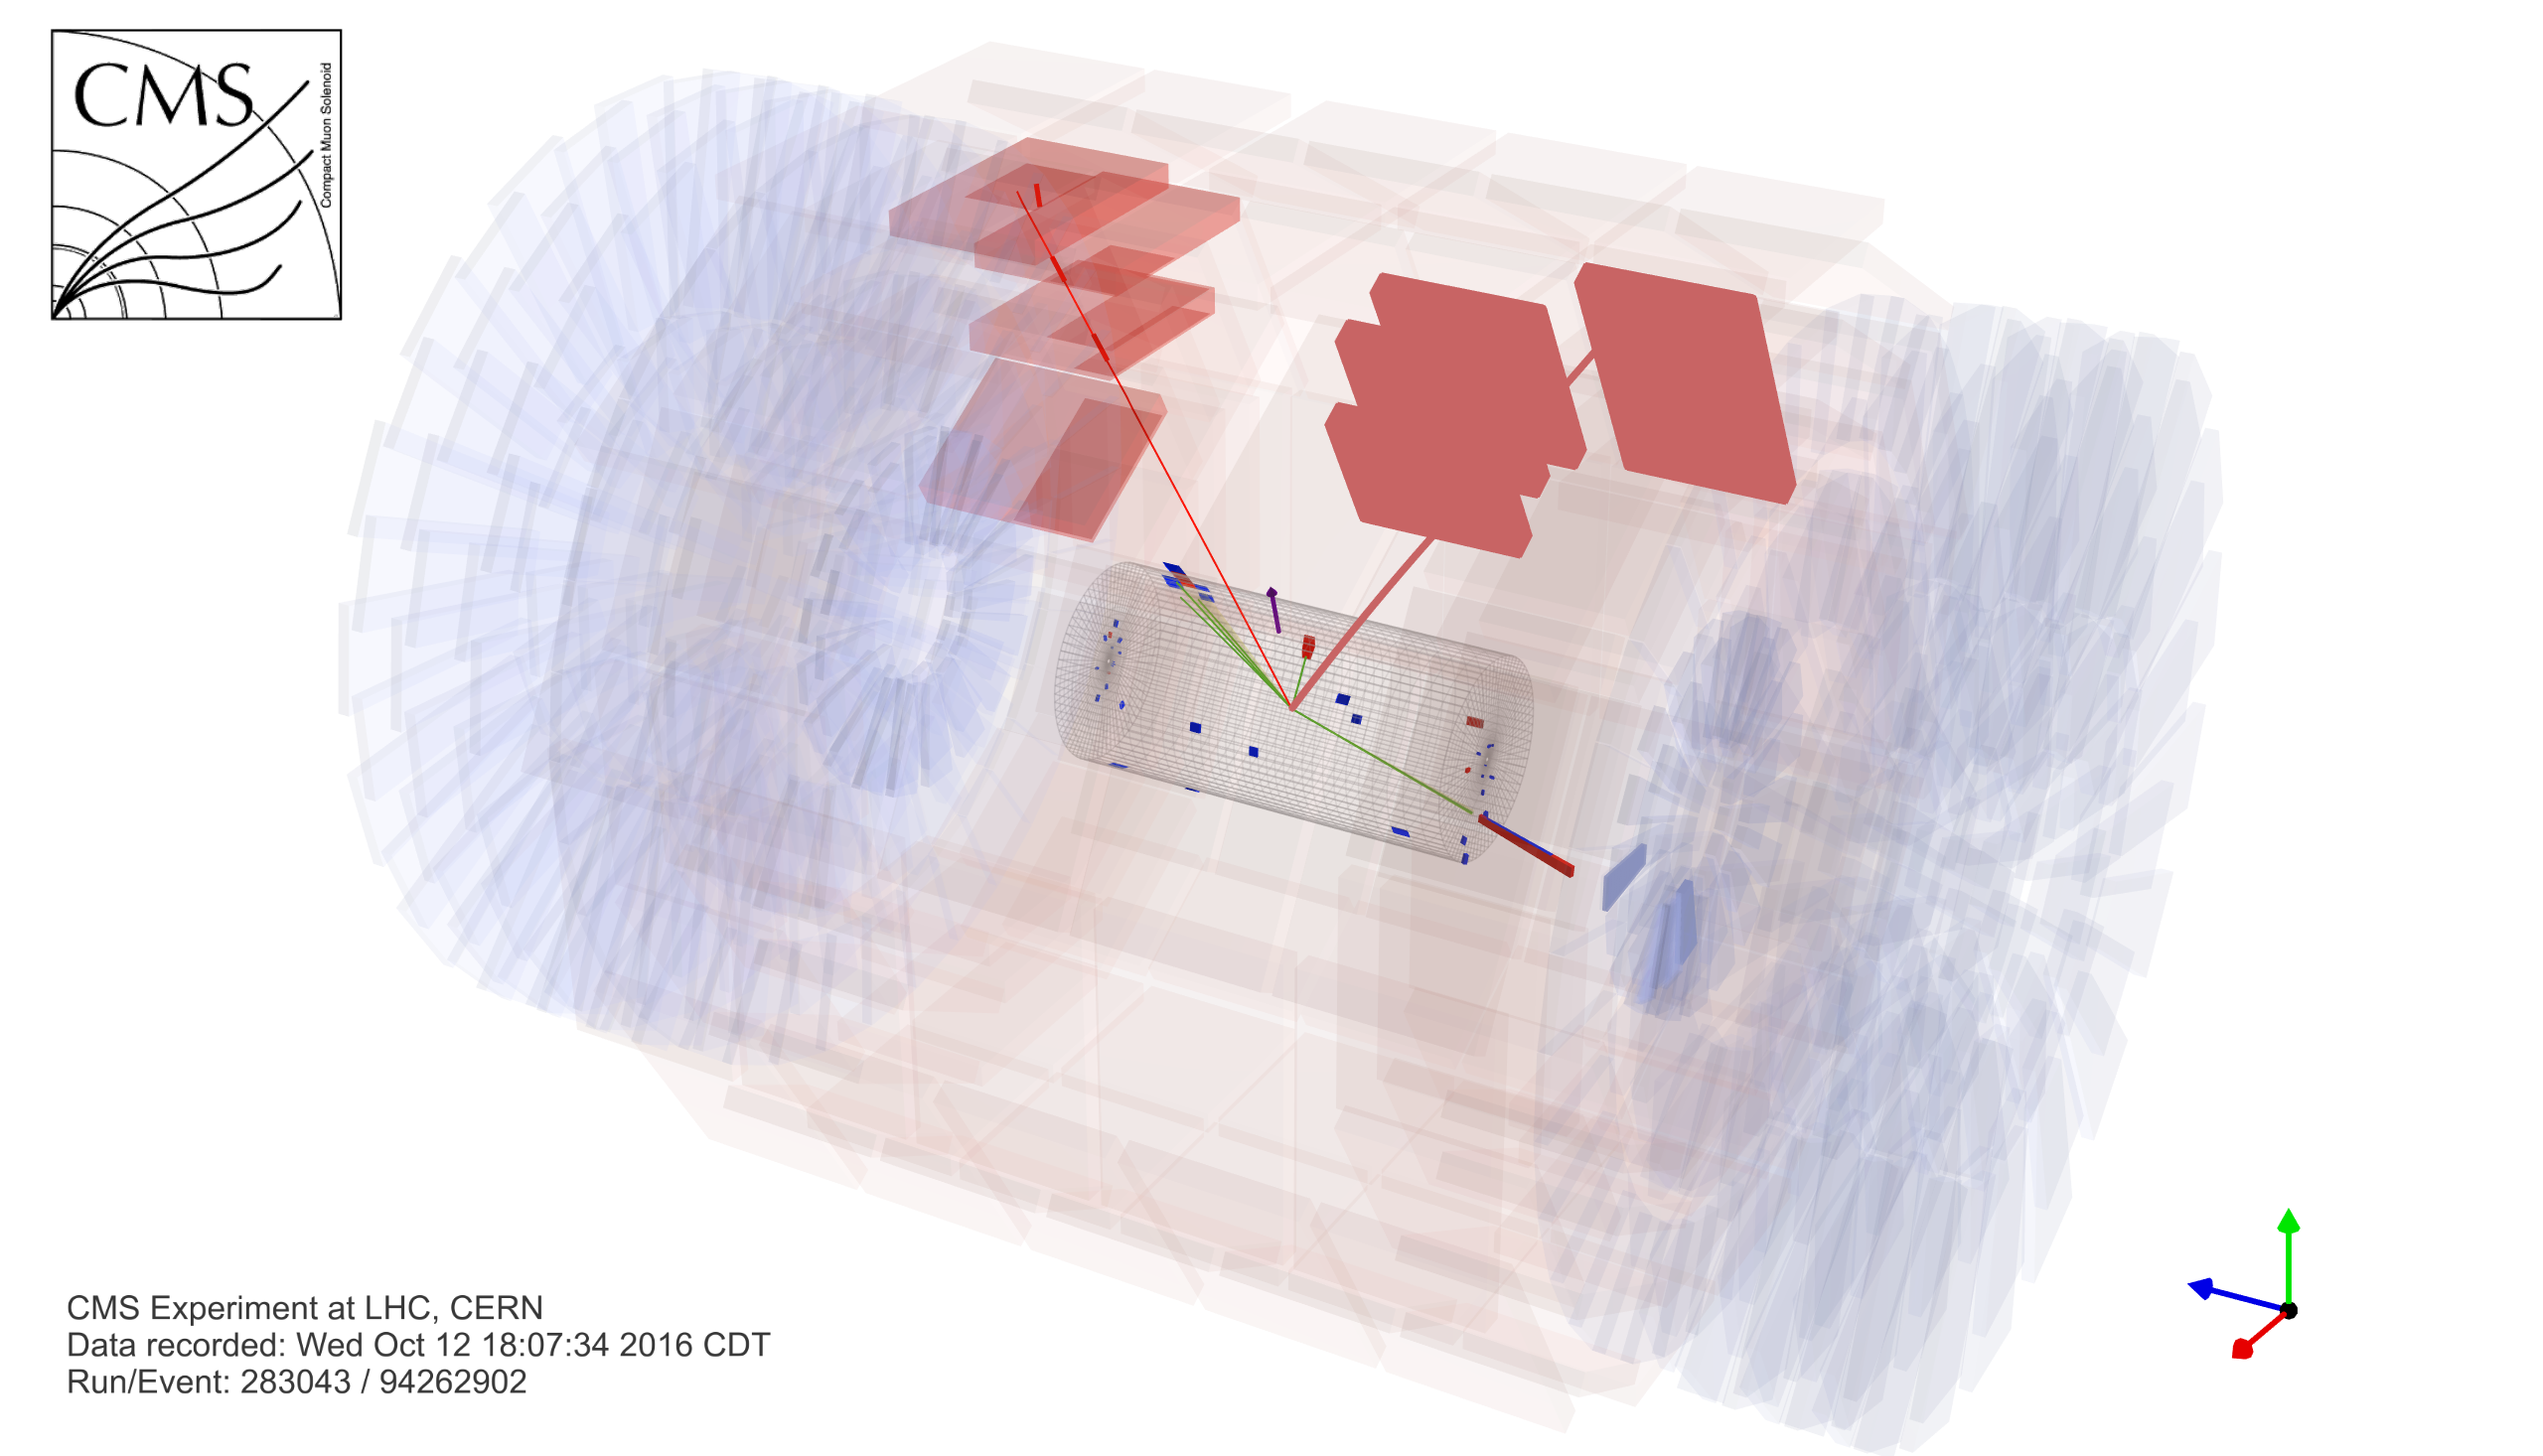
\includegraphics[width=0.95\textwidth]{figures/AnalysisProcedure/WZjjFullEventView.png}
  \caption[Visualization of a selected \EWWZ candidate event]{
    Visualization of a candidate \EWWZ event selected by in this analysis. High momentum
    and well separated jets are observed in the forward part of the detector. Two muons
    (red) satisfy the $\pt$ requirements while forming a composite object with invariant
    mass consistent with $m_{\PZ}$. Moderate missing transverse momentum (purple arrow)
    and an electron candidate (light blue) are consistent with a $\PW$-boson decay.
        }
 \label{fig:eventView}
\end{figure}

Deviation from the SM prediction in the rate of \EWWZ production, 
or in kinematic distributions sensitive to the scattering energy of the process,
such as $m_{WZ}$, could indicate the presence of BSM physics.
This section describes the selection of events, the estimation of 
the expected signal and background contributions, the assessment of
systematic uncertainties impacting these estimations, and the statistical
techniques used to derive results. Results are presented in both SM
and BSM interpretations, as described in Chapter~\ref{ch:phenomenology}.

\section{Background composition}

Several process can mimic the $\WZjj\rightarrow3\ell\jet\jet$ signal. 
For the \EWWZ
selection described in Section~\ref{sec:eventselection},
true \WZjj production is estimated to account for $3/4$ of the
expected event yield, with background processes accounting
for $1/4$ of the expected events. The estimation of each
background contribution is discussed in 
Sections~\ref{sec:promptbackgrounds} and~\ref{sec:nonpromptbackgrounds}.

We refer to processes 
with at least three leptons produced in the hard scattering interaction
as ``prompt.'' This includes the leptonic decay channels of 
$\PZ\PZ$, \tZq, $\ttbar\cPZ$, and VVV production,
where V refers to a $\PW$ or $\PW$ boson. The \tZq process, where
the top quark decays leptonically via a $\PW$ boson, is the dominant
prompt background contribution, accounting for
$~25\%$ of background events after the \EWWZ selection. 
In this process, 
one vector boson is radiated from the incoming quark,
leading to a forward jet in addition to the three lepton signature.
The $\PZ\PZ\jet\jet$, $\ttbar\cPZ$, and VVV processes
enter the \WZjj selection when leptons
are outside of the detector acceptance, leading to the three lepton and
\ptmiss signature. The $\ttbar\cPZ$, $\PZ\PZ$, and $\cPZ\cPZ$ processes
are estimated to account for about 15\%, 10\%, and 5\% of the total
background respectively.

``Nonprompt'' processes arise when leptons which are produced outside
the hard interaction, especially through leptonic decays of hadronic
states in jets and photon conversion to leptons in the detector material.
These processes are dominated by $\cPZ$+jet production, in which
misidentification and mismeasurement of jet activity mimics
a third lepton and gives rise to $\ptmiss$ in the event, \ttbar production,
and $\PZ\gamma$ production. The expected contributions from these 
processes are 30\%, 5\%, and 10\% of the total background for events
satisfying the \EWWZ signal selection.

The component of the \WZjj process considered as signal or background
is adjusted for the interpretation of results. For the \WZjj fiducial
cross section measurement, all SM \WZjj production mechanisms are considered 
signal.
For the \EWWZ measurement,
the \EWWZ process is considered signal, and the \QCDWZ process is considered
background. The \QCDWZ process is the dominant background in this search,
with a ratio of $~3:1$ to the \EWWZ process in the signal region.
For new physics searches, all SM \WZjj processes are considered background.
The ratio of \EWWZ and \QCDWZ processes is assumed to be consistent with the SM
expectation.

\section{Event triggering}

Collision events are selected by triggers that require the presence of
one or two electrons or muons.
The \pt threshold for the single lepton trigger is 25 (20)\GeV for the electron (muon) trigger.
For the dilepton triggers, with the same or different flavors, the minimum \pt of the leading and subleading leptons are 17\,(17) and 12\,(8)\GeV
for electrons (muons), respectively.
The combination of these trigger paths brings the trigger efficiency for three-lepton events
satisfying the minimum $\pt$ requirements to nearly 100\%.
However, partial mistiming of signals in the forward region of the electromagnetic calorimeter (ECAL) endcaps
($2.5 < \left|\eta\right| < 3.0$) led to a reduction in the level 1 trigger efficiency. 

Larger-than-expected aging effects in ECAL crystals altered the 
energy pulse shape of signals in the ECAL, leading to
early event readout for a significant fraction of events
with high electromagnetic activity in the ECAL endcaps towards the end
of 2016 data taking.
This effect, known as pre-firing, is significant because requirements necessary
to avoid excessive data readout prevent events from successive bunch crossings
from being accepted by the CMS trigger system. 
That is, if an event has been accepted by the CMS trigger
system, it is impossible for the following event to also be accepted.

In normal conditions, the inefficiency due to this requirement is very small
and unbiased. Systematic pre-firing, however, can lead to a biased and unrecoverable
loss of efficiency.
For \EWWZ events, mistiming of ECAL trigger objects in
forward and high momentum jets can lead to such L1 pre-firing.
The jet leading to pre-firing is incorrectly associated with the previous bunch
crossing, producing an event missing the leptonic signature of \WZ events.
The triggered event is likely to be rejected by the HLT, while the correctly-timed
event is rejected by the restriction against successive triggered events.

A correction for this efficiency loss with respect to the expectation in the MC simulation 
is determined using an unbiased sample
of events in which the event pre-firing is prevented by additional trigger conditions.
In particular, a sample of events is selected where the trigger conditions
restricting the readout of events separated by less than three bunch crossings 
prevented the mistimed electromagnetic
signal from firing the trigger, but did not prevent the correctly timed event
from triggering. This sample of events is formed by selecting 
jet candidates in the reconstructed data, defined 
using the anti-$\kt$ algorithm and required to have $\pt > 30\GeV$,
which are matched to their trigger primitive objects.
The jet pre-firing efficiency is defined as the ratio of events with jets
matched to an L1 trigger object associated with the correct bunch crossing 
to the all events with selected jets. 
For jets with $\abs{\eta} < 2.25$, the pre-firing rate is less than 2\% 
over the entire \pt spectrum. In contrast, it
grows as a function of jet \pt and $\eta$ up to values close to 100\% 
for jets with $2.75 < \abs{\eta} < 3.0$ and $\pt > 400\GeV$.

\begin{figure}[htbp]
  \centering
   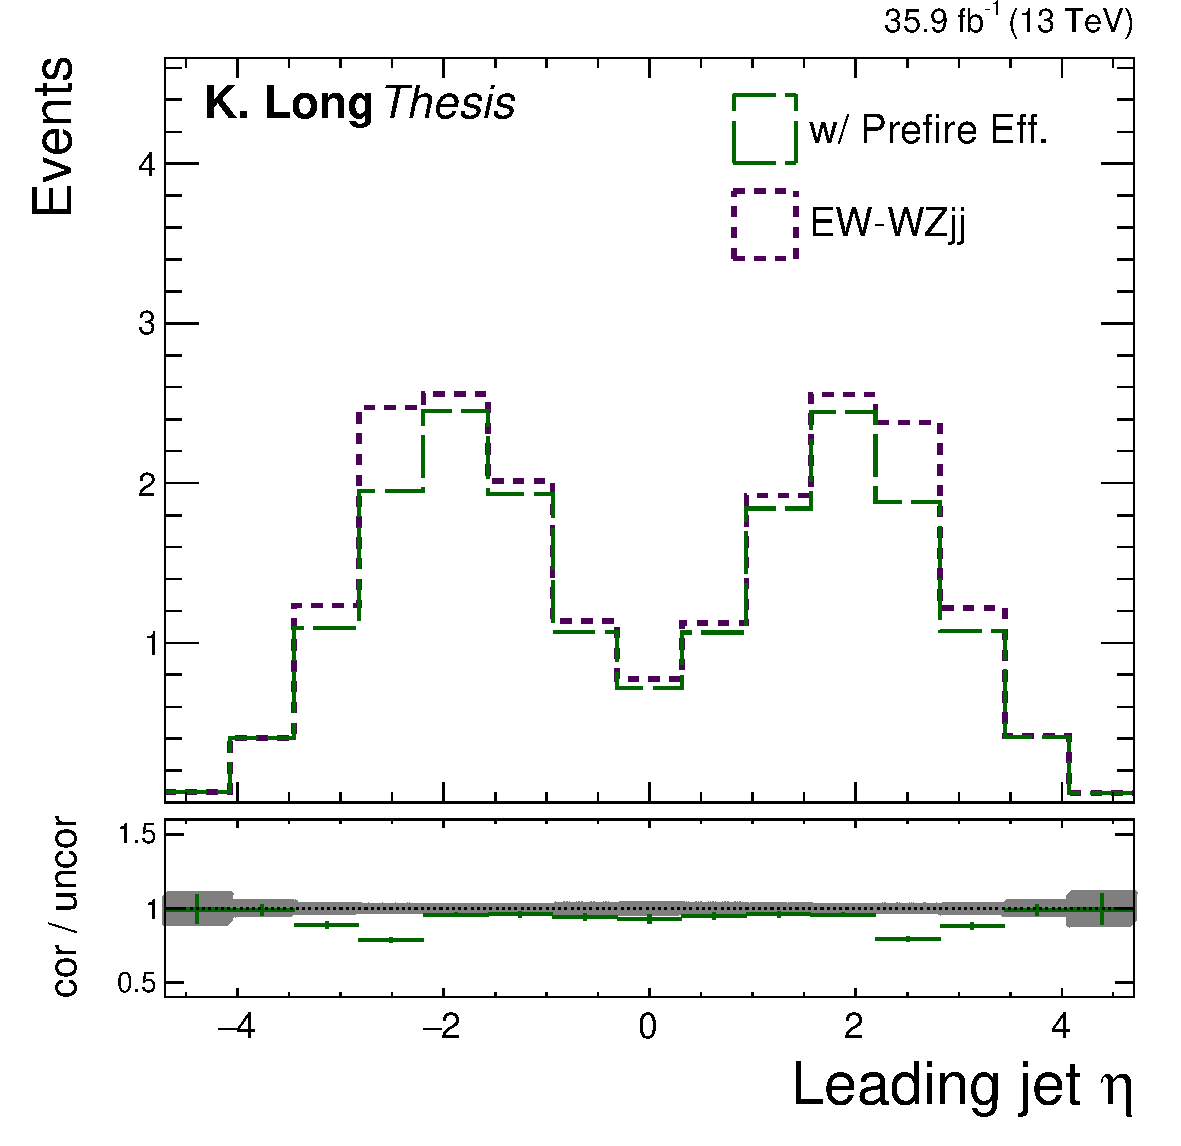
\includegraphics[width=0.45\textwidth]{figures/AnalysisProcedure/jet0Eta_prefiring.pdf}
   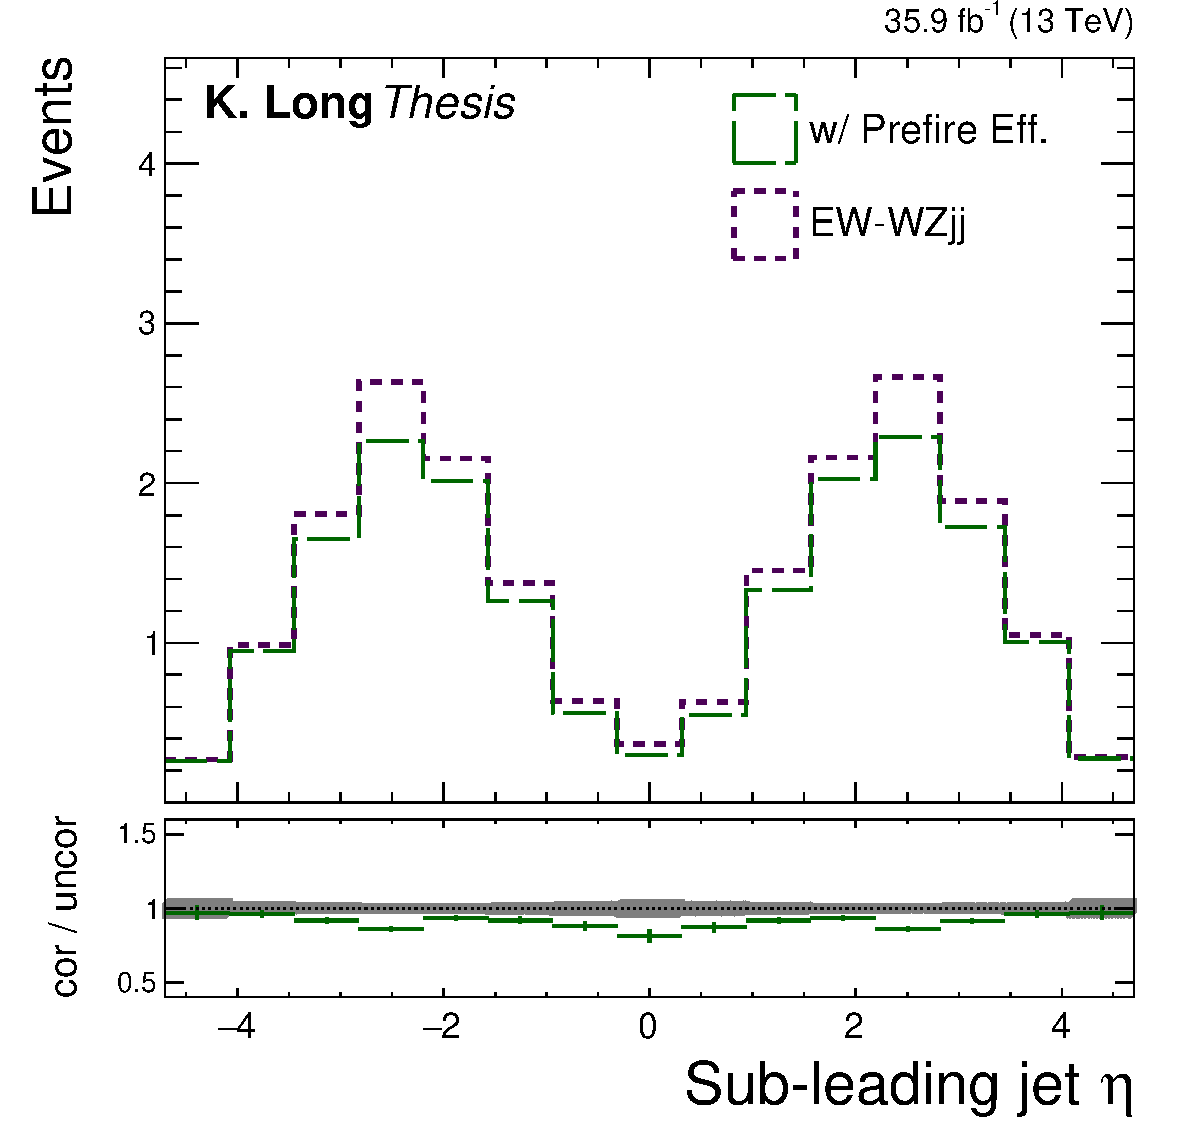
\includegraphics[width=0.45\textwidth]{figures/AnalysisProcedure/jet1Eta_prefiring.pdf}
   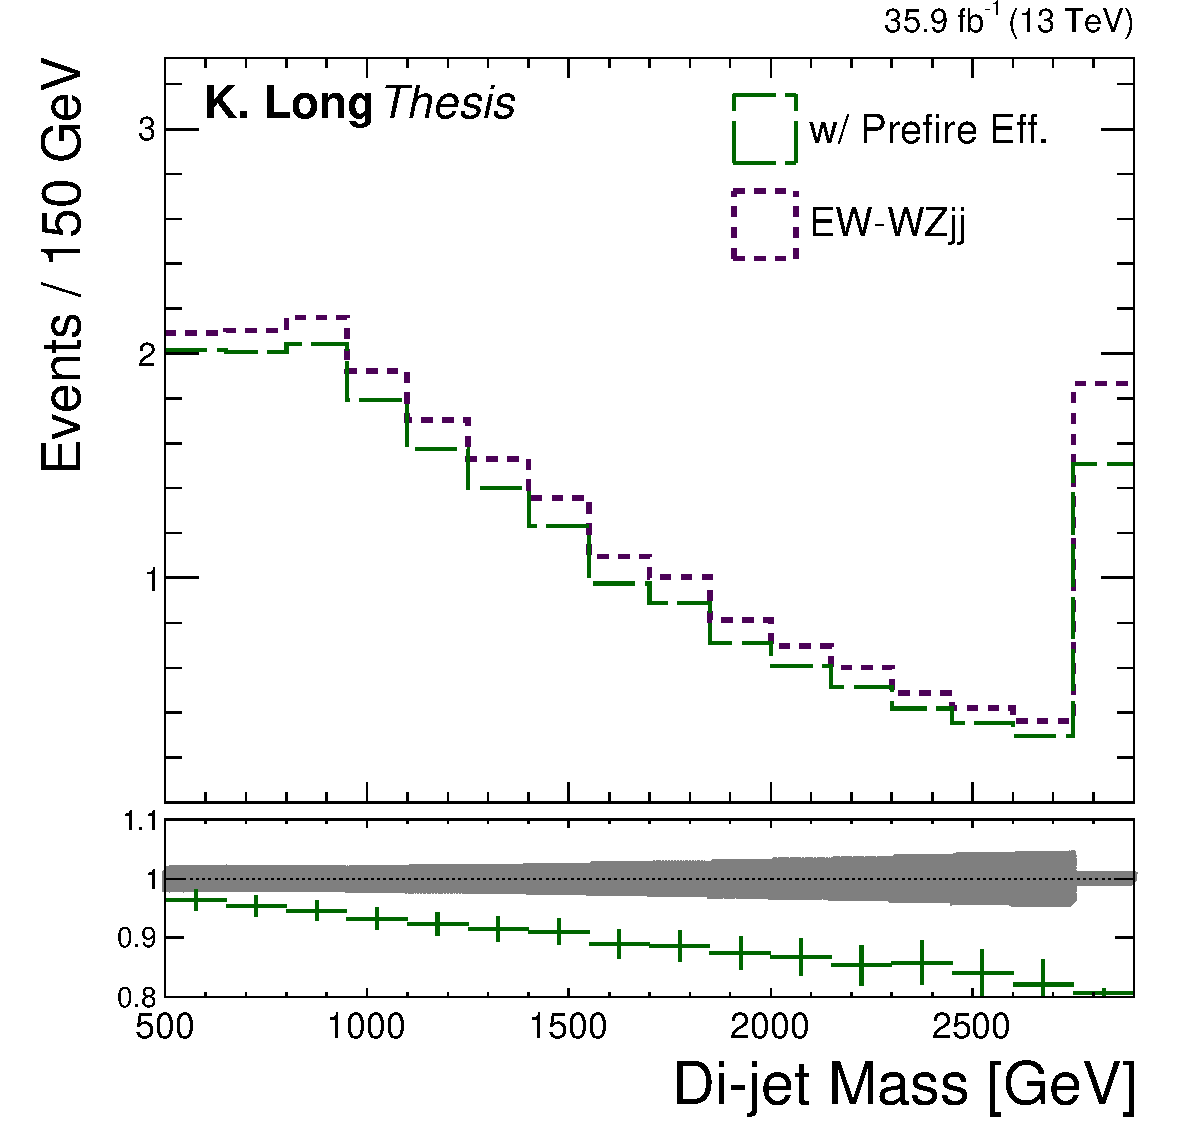
\includegraphics[width=0.45\textwidth]{figures/AnalysisProcedure/mjj_prefiring.pdf}
   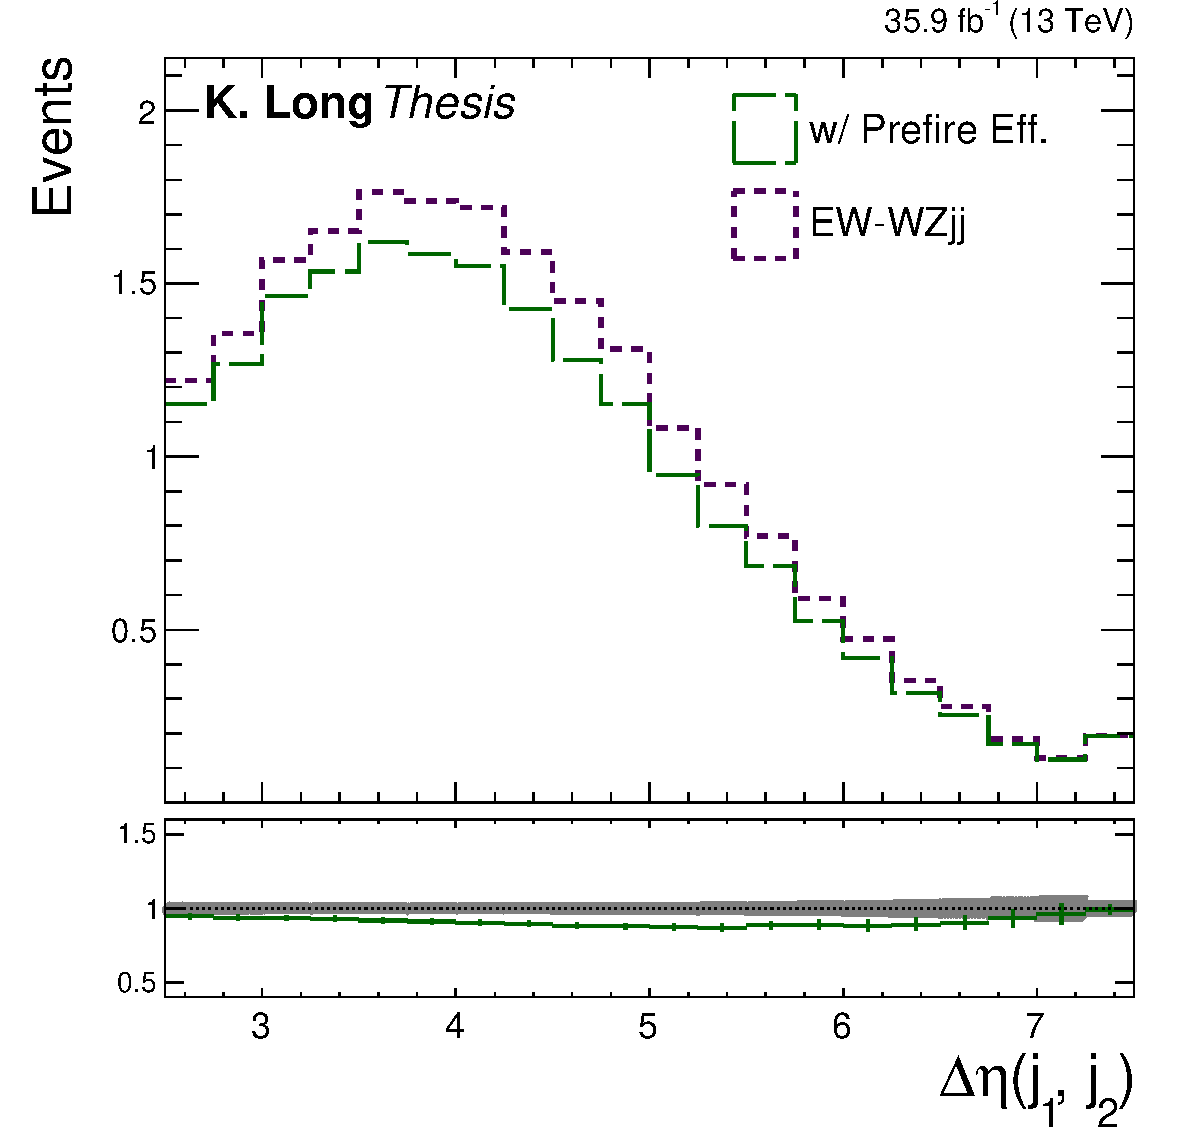
\includegraphics[width=0.45\textwidth]{figures/AnalysisProcedure/dEtajj_prefiring.pdf}
  \caption[Estimated efficiency loss for selected \EWWZ simulated events due to 
      mistimed events in the L1 trigger]{
      Estimated efficiency loss for selected \EWWZ simulated events due to 
      mistimed events in the L1 trigger. The solid lines show the uncorrected
      distributions, while the dotted lines show the efficiency-corrected 
      predictions.
        }
 \label{fig:signalPrefiringEff}
\end{figure}

The impact of this inefficiency on this analysis is estimated by applying
these efficiency corrections, estimated in bins of jet $\pt$ and $\eta$,
to the selected signal and background events. Due to the signature of forward
and high momentum jets, the \EWWZ process is particularly affected. 
This is demonstrated in Fig.~\ref{fig:signalPrefiringEff}, which shows the
estimated efficiency loss in jet $\eta$, $\mjj$, and $\detajj$
for simulated \EWWZ events selected for the analysis.
This loss of efficiency is found to be about 
1\% for {\mjj} of $200\GeV$ and it increases to about 15\% for $\mjj > 2\TeV$.
The loss of sensitivity due to this inefficiency in the \EWWZ search is estimated 
to be about 10\%. 

\section{Event selection and fiducial cross section regions}
\label{sec:eventselection}

A selected event is required to have three lepton candidates $\ell\ell'\ell'$,
where $\ell, \ell' = \mathrm{e}$, $\mu$.
All leptons
must pass the identification and isolation requirements
described in Chapter~\ref{ch:reconstruction}.
The electrons and muons can be directly produced from a {\PW} or {\cPZ} boson decay or from a {\PW} or {\cPZ}
boson with an intermediate $\tau$ lepton decay.
The $\ell'\ell'$ pair consists of two leptons with opposite charge and the same flavor,
as expected for a $\cPZ$ boson candidate.
One of the leptons from the $\cPZ$ boson candidate is required to have $\pt^{\ell'_{1}} > 25\GeV$ and the other
$\pt^{\ell'_{2}} > 15\GeV$.
For events with three same-flavor leptons, two oppositely charged, same-flavor combinations are possible.
The pair with invariant mass closest to $m_{\cPZ} = 91.2\GeV$, the nominal $\cPZ$ boson mass from
Ref.~\cite{Tanabashi:2018oca}, is selected as the $\cPZ$ boson candidate.
The remaining lepton is associated with the $\PW$ boson and must have $\pt^{\ell} > 20\GeV$.
Events containing additional isolated leptons with $\pt^{\ell} > 10\GeV$ are rejected.
Because of the neutrino in the final state, the events are required to have $\ptmiss > 30\GeV$.
To reduce contributions from $\ttbar$ events,
the leptons constituting the $\cPZ$ boson candidate are required to have an invariant mass satisfying
$\abs{m_{\ell'\ell'} - m_\cPZ} < 15\GeV $ and events with a
{\cPqb} tagged jet with $\pt^{\cPqb} > 30\,\GeV$ and $\abs{\eta^{\cPqb}} < 2.4$ are vetoed.

\begin{figure}[htbp]
  \centering
   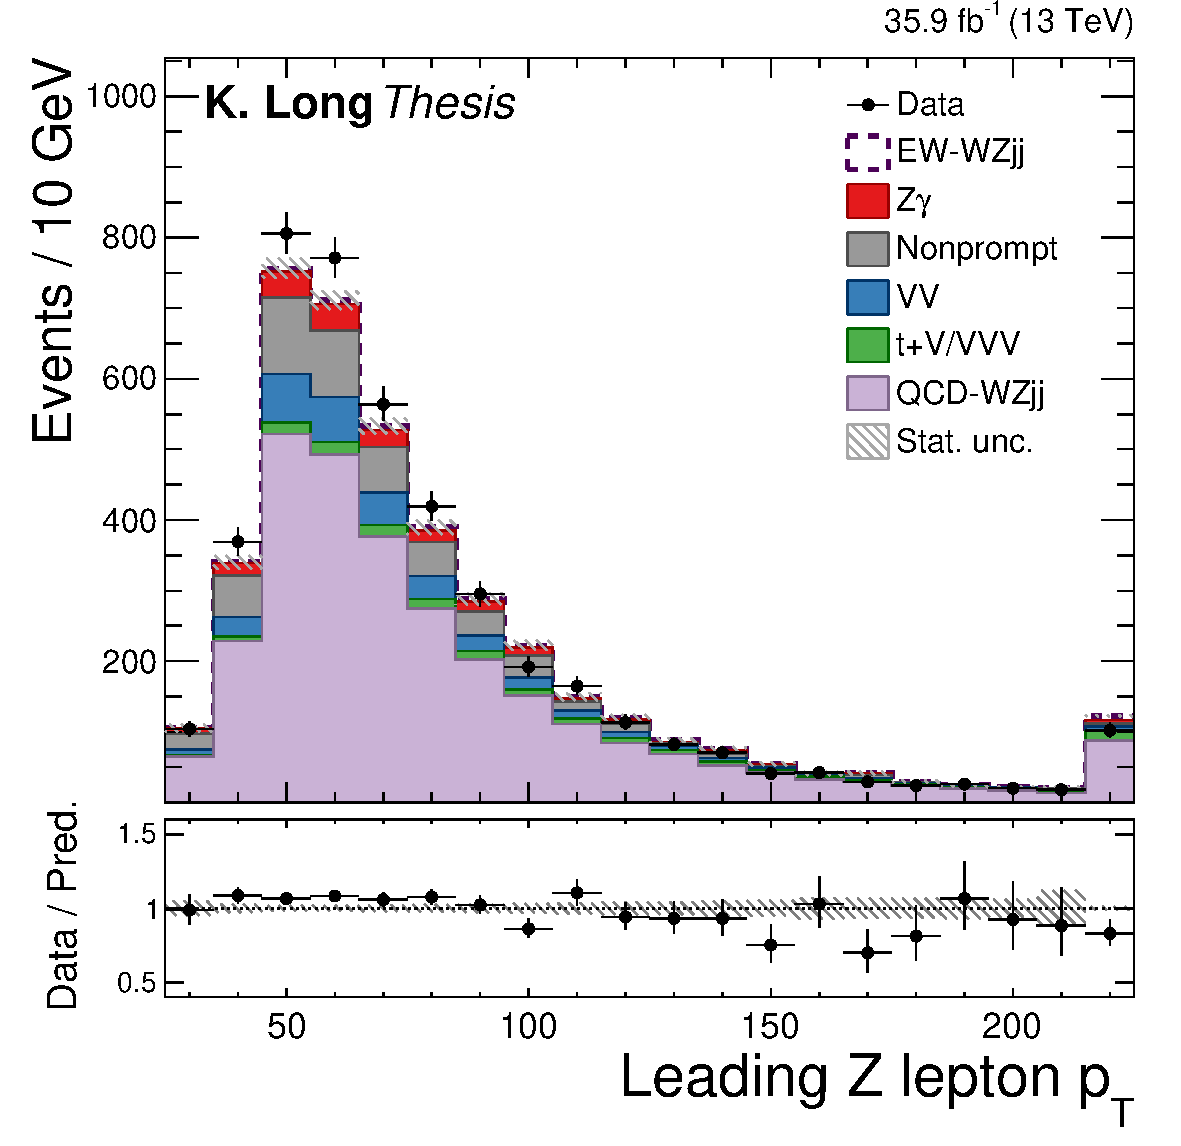
\includegraphics[width=0.4\textwidth]{figures/AnalysisProcedure/Zlep1_Pt_Wselection.pdf}
   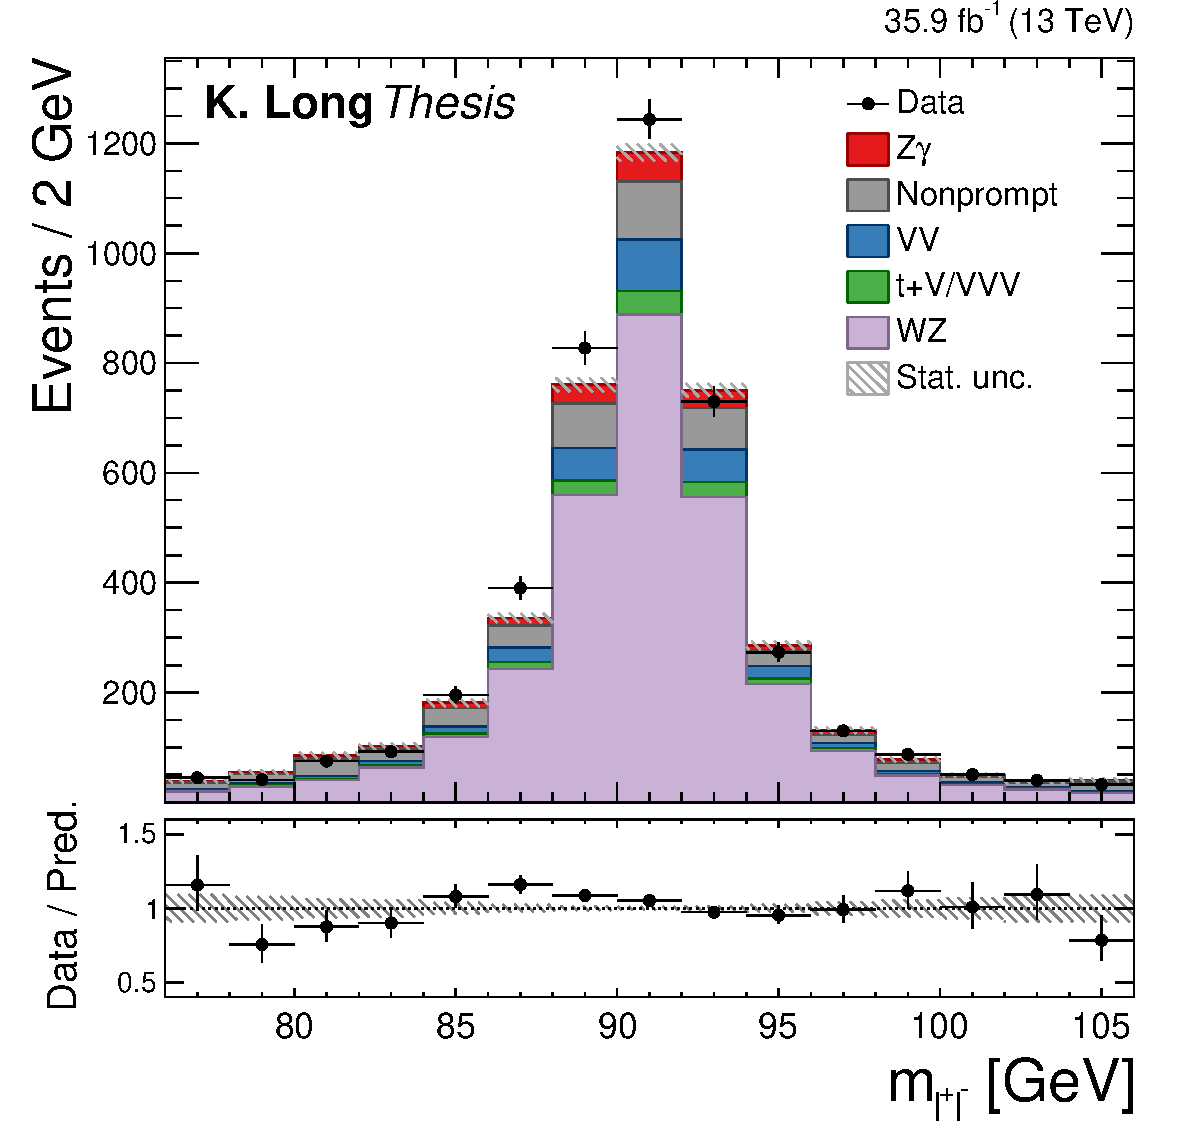
\includegraphics[width=0.4\textwidth]{figures/AnalysisProcedure/ZMass_Wselection.pdf}
   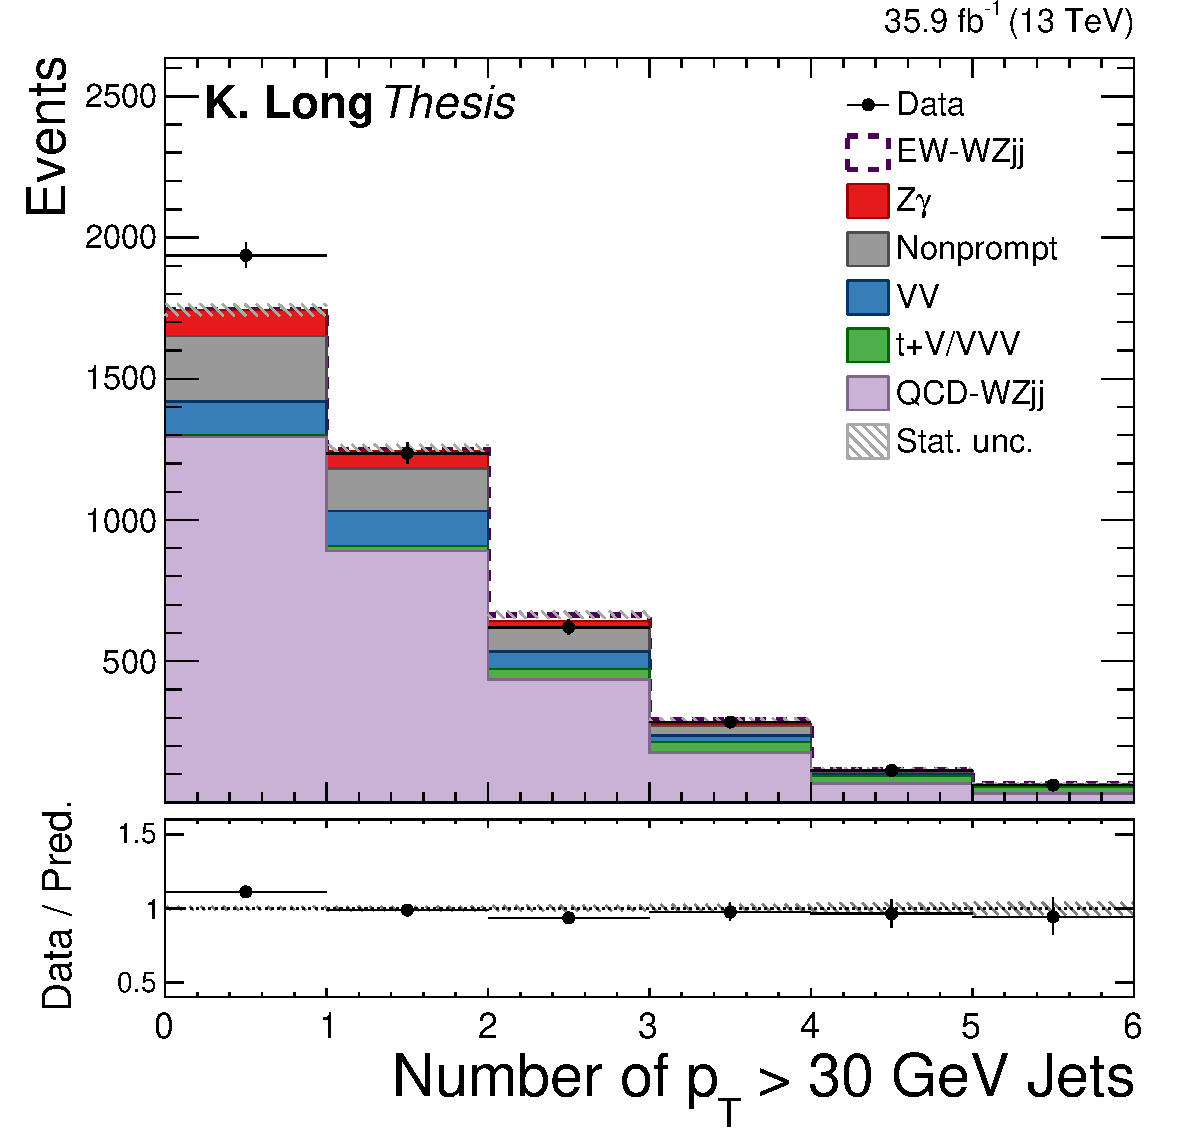
\includegraphics[width=0.4\textwidth]{figures/AnalysisProcedure/nJets_Wselection.pdf}
   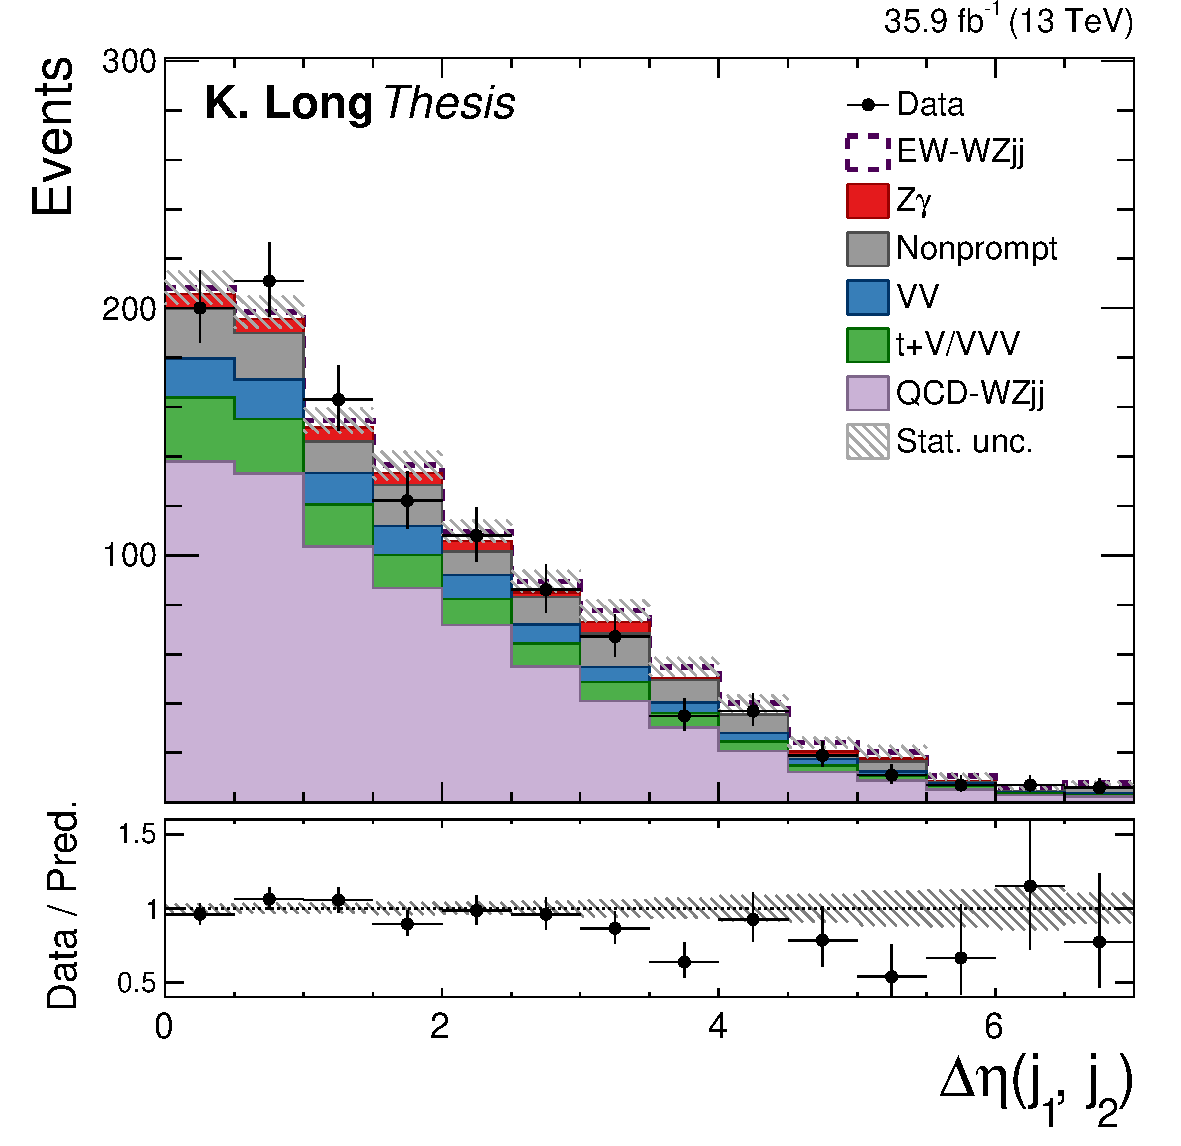
\includegraphics[width=0.4\textwidth]{figures/AnalysisProcedure/dEtajj_Wselection.pdf}
  \caption[Distributions for events satisfying the \WZ selection]{
    Distributions for events satisfying the \WZ selection described in the text.
    The $\pt$ of the highest momentum lepton associated with the $\PZ$ boson 
    candidate (top left), the invariant mass of the $\PZ$ candidate (top right),
    and the event rate by number of anit-$\kt$ jets with $\pt > 30\GeV$ (bottom left)
    are shown with no requirement on the jet activity in the event. The rapidity
    Separation of the highest $\pt$ jets for events with at least two
    $\pt>30\GeV$ events are also shown (bottom right).
        }
 \label{fig:WselectionPlots}
\end{figure}

The invariant mass of any dilepton
pair $m_{\ell\ell}$ must be greater than 4\GeV.
Such a requirement is necessary in theoretical calculations to avoid divergences
from collinear emission of same-flavor opposite-sign
dilepton pairs, and 4\GeV is chosen to avoid low mass resonances
and double semileptonic decays of B and D hadrons.
The selection is extended to all dilepton pairs to
reduce contributions from backgrounds with soft leptons while having a negligible effect on signal efficiency.
The trilepton invariant mass, $m_{3\ell}$, is required to be more than 100\GeV
to exclude a region where production of $\cPZ$ bosons with final-state photon radiation
is expected to contribute. Such events enter the signal region when the radiated photon
pair converts to electrons and one electron is lost.

Distributions of events satisfying these criteria, designed to select
$\WZ\rightarrow 3\ell\nu$ events, are shown in Fig.~\ref{fig:WselectionPlots}.
The \WZ production rate by
number of anti-$\kt$ jets, and the rapidity separation of the two
highest $\pt$ jets for events with at least two anit-$\kt$ jets
with are also shown.

With no condition on the jet activity in the selection,
the \EWWZ contribution is negligible. To enhance the \EWWZ contribution,
the event must have at least two jets with $\pt > 30\GeV$ and $|\eta| < 4.7$. 
The jet with the highest $\pt$ is 
called the leading jet and the jet with the second-highest $\pt$ the subleading jet. 
To exploit the unique signature of the VBS process, these two jets are required to have
$\mjj > 500\GeV$ and $\eta$ separation 
$\left|\detajj \right| \equiv \left|\etajj \right| > 2.5$.
This selection 
is used for searches for charged Higgs bosons and therefore called the ``Higgs boson selection."
For the \WZjj and \EWWZ measurement,
the leading and subleading jet must satisfy $\pt > 50\GeV$, and
the variable $\etas = \zepl$
of the three-lepton system is additionally required to be between $-2.5$ and 2.5. This selection is
referred to as the ``EW signal selection." 
A summary of these selections is shown in Table~\ref{tab:selections}. 

\begin{table*}[!ht]
  \centering
  \caption[Summary of event selections and fiducial region definitions for the analysis]
  {Summary of event selections and fiducial region definitions for the analysis.
    The selections labeled ``EW signal'' and ``Higgs boson'' are applied to data and reconstructed
    simulated events.
    The EW signal selection is used for all measurements except for the charged Higgs boson search that
    uses the selection indicated in the column labeled ``Higgs boson.''
    The \WZjj cross section is reported in the fiducial regions defined by the selections specified in
    the last two columns applied to particle-level simulated events. The variables
    $n_{\jet}$ and $n_{\cPqb}$ refer to the number of
    anti-\kt jets and the number of anti-\kt \cPqb-tagged jets,
    respectively. Other variables are defined in the text.
    }
  \begin{tabular}{ccccc}
  \hline
                                           &  EW signal & Higgs boson & Tight fiducial & Loose fiducial \\
  \hline
  $  \PT^{\ell'_{1}}   $            [GeV]  &  $>$25     & $>$25        & $>$25         & $>$20          \\
  $  \PT^{\ell'_{2}}   $            [GeV]  &  $>$15     & $>$15        & $>$15         & $>$20          \\
  $  \PT^{\ell}     $               [GeV]  &  $>$20     & $>$20        & $>$20         & $>$20          \\
  $\abs{\eta^{\mu}}   $                    &  $<$2.4    & $<$2.4       & $<$2.5        & $<$2.5         \\
  $\abs{\eta^{\mathrm{e}}}$                &  $<$2.5    & $<$2.5       & $<$2.5        & $<$2.5         \\
  $\abs{m_{\ell'\ell'}-m_{\cPZ}}$   [GeV]  &  $<$15     & $<$15        & $<$15         & $<$15          \\
  $m_{3\ell}                $       [GeV]  &  $>$100    & $>$100       & $>$100        & $>$100         \\
  $m_{\ell\ell}           $         [GeV]  &  $>$4      & $>$4         & $>$4          & $>$4           \\
  $\ptmiss                  $       [GeV]  &  $>$30     & $>$30        & \NA           &   \NA          \\
  $\abs{\eta^{\jet}}  $                    &  $<$ 4.7   & $<$4.7       & $<$4.7        & $<$4.7         \\
  $\PT^{\jet}                $      [GeV]  &  $>$50     & $>$30        & $>$50         & $>$30          \\
  $\abs{\Delta R(\jet, \ell)}$             &  $>$0.4    & $>$0.4       & $>$0.4        & $>$0.4         \\
  $n_{\jet}           $                    &  $\ge$2    & $\ge$2       & $\ge$2        & $\ge$2         \\
  $\PT^{\cPqb}          $           [GeV]  &  $>$30     & $>$30        &   \NA         &   \NA          \\
  $\abs{\eta^{\cPqb}}  $                   &  $<$2.4    & $<$2.4       &   \NA         &   \NA          \\
  $n_{\cPqb}       $                       &  $=$0      & $=$0         &   \NA         &   \NA          \\
  $\mjj             $                      &  $>$500    & $>$500       & $>$500        & $>$500         \\
  $\abs{\etajj }$                          &  $>$2.5    & $>$2.5       & $>$2.5        & $>$2.5         \\
  $\abs{ \zepl }$                          &  $<$2.5    & \NA          & $<$2.5       & \NA            \\
  \end{tabular}
  \label{tab:selections}
\end{table*}

To reduce the dependence on theoretical predictions,
measurements are reported in two fiducial regions, defined in Table~\ref{tab:selections}.
The ``tight fiducial region'' is defined to be as close as possible to the measurement phase space,
whereas the ``loose fiducial region'' is designed to be easily reproducible
in theoretical calculations or in MC simulations, following the procedure of
Ref.~\cite{leshouches2017}.
The fiducial predictions are defined through selections on particle-level
simulated events using the \Rivet~\cite{Buckley:2010ar} framework, which
provides a toolkit for analyzing simulated events in a model-independent way.
Electrons and muons are required to be prompt (i.e., not from hadron decays),
and those produced in the decay of a $\tau$ lepton
are not considered in the definition
of the fiducial phase space.
The momenta of prompt photons located within a cone of radius $\Delta R = 0.1$ are added to the lepton
momentum to correct for final-state photon radiation, referred to as ``dressing.''
The three highest \pt leptons are selected and associated with the {\PW} and {\cPZ}
bosons with the same procedure used in the data selection.
The fiducial cross section in the \QCDWZ sideband region is defined
following the tight fiducial region of Table~\ref{tab:selections},
with $\mjj > 100\GeV$ and $\mjj < 500\GeV$ or $\abs{\etajj} < 2.5$ or $\abs{\etas} > 2.5$.
Theoretical predictions are evaluated using \MG at LO interfaced to \PYTHIA with the samples
described in Section~\ref{sec:promptbackgrounds}.

\section{Background contributions}
Background contributions in this analysis are divided into two categories:
background processes with prompt isolated leptons, \eg, 
$\PZ\PZ$, \tZq, $\ttbar\cPZ$;
and background processes with nonprompt leptons from hadrons decaying to leptons inside jets or
jets misidentified as isolated leptons, primarily $\ttbar$ and $\cPZ$+jets.
The background processes with prompt leptons are estimated from MC simulation, while backgrounds
with nonprompt leptons from hadronic activity are estimated from control samples in data.
The nonprompt component of the $\cPZ\gamma$ process,
in which the photon experiences conversion into leptons in the tracker,
is evaluated using MC simulation. 

\subsection{Signal simulation and estimation of prompt backgrounds}
\label{sec:promptbackgrounds}

Several Monte Carlo (MC) event generators are used to simulate the signal and
background processes.

The EW-induced production of \WZ boson pairs and two final-state quarks, where the W and Z bosons decay leptonically, 
is simulated at leading order (LO) in perturbative QCD using 
\MG v2.4.2~\cite{MGatNLO}. 
The sample includes all contributions to the four-lepton final state at $\mathcal{O}(\alpha^6)$ and 
with a resonant W boson propagator, including
triboson processes, where the \WZ boson pair is accompanied by 
a third vector boson that decays into jets, as well as diagrams involving the quartic coupling vertex. 
The resonant W boson is decayed using {\sc MadSpin}~\cite{Artoisenet:2012st}.
Contributions with an initial-state b quark are excluded from the sample
as they are considered part of the \tZq process.
The predictions from this sample are cross-checked with LO predictions from the 
event generators \VBFNLO~3.0~\cite{VBFNLO} and 
\Sherpa~v2.2.4~\cite{Gleisberg:2008ta,Gleisberg:2003xi}, 
and with fixed-order calculations from
\Moca~\cite{leshouches2017,Recola}. Agreement is obtained when using equivalent configurations
of input parameters, including couplings, particle masses and widths, and the choice of
renormalization ($\mu_{R}$) and 
factorization scales ($\mu_{F}$),
and differences arising from such configurations are considered when assessing the uncertainty.

Several MC simulations of the \QCDWZ process are considered.
The simulations are inclusive in the number of jets associated with the 
leptonically decaying \PW and {\cPZ} bosons, and therefore include 
the \WZjj contribution studied in this analysis.
The primary MC sample is simulated at 
LO with \MG v2.4.2, with contributions to \WZ production with up to three outgoing partons 
included in the matrix element calculation. 
The different jet multiplicities are merged using the MLM scheme~\cite{MLMmerging}.
A next-to-LO (NLO) sample from \MG v2.3.3 
with zero or one outgoing partons at Born level, merged using the \FxFx scheme~\cite{Frederix:2012ps},
and an inclusive NLO sample from \POWHEG2.0~\cite{Melia:2011tj,Nason:2004rx,Frixione:2007vw,powheg:2010}
are also considered. 
The LO MC with MLM merging, referred to as the MLM-merged sample, 
is taken as the central prediction due its inclusion of
\WZ plus three-parton contributions at tree level, which are relevant
to \WZjj production.
The other samples,
which are used to access the modeling uncertainty in the \QCDWZ process,
are referred to as the \FxFx-merged
and the \POWHEG samples, respectively.
Each sample is scaled to the inclusive NLO cross section from \POWHEG2.0.

The contribution from \QCDWZ production is estimated with MC simulation.
It is considered signal for the \WZjj cross section measurement,
but is the dominant background for the \EWWZ measurement and in searches for
new physics.
For the \EWWZ measurement
and new physics searches, the normalization of the \QCDWZ process is
constrained by data in the \QCDWZ sideband region.
The cross section predicted by the MLM-merged sample
in the \QCDWZ sideband region is
$18.6 \,^{+2.9}_{-2.3}\scale \pm 1.0\PDF\unit{fb}$,
where the scale and PDF uncertainties are calculated using the procedure
described in Section~\ref{sec:systematics}.
In this region the normalization correction, which is derived from a fit to the data, is
consistent with unity.
The \EWWZ process, considered signal for the \WZjj and \EWWZ
measurements but background to new physics searches, is also
estimated using MC simulation.

In addition to the \EWWZ and \QCDWZ process, which at tree level are 
$\mathcal{O}(\alpha^4)$ and $\mathcal{O}(\alpha^2\alpha_{S}^2)$ respectively,
a smaller contribution at $\mathcal{O}(\alpha^3\alpha_{S})$ 
contributes to the \WZjj state. We refer to this contribution as the 
interference term. It amounts to less than 5\% of the signal in the \EW signal selection
and is taken as an uncertainty on the signal contribution.
It is evaluated using samples of particle-level
events generated with \MG v2.6.0. Samples are generated with the dynamic $\mu_{R}$
and $\mu_{F}$ set to the maximum of the parton transverse momenta per event, and with fixed
scales $\mu_{R} = \mu_{F} = m_{\mathrm{W}}$, where $m_{\mathrm{W}}$ is the world average value of the 
W boson mass, taken from Ref.~\cite{Tanabashi:2018oca}.

The associated production of a $\PZ$ boson and a single top quark, referred to as \tZq production,
is simulated at NLO in the four-flavor scheme using \MG v2.3.3. 
The sample is scaled using a cross section computed at NLO with \MG in the five-flavor scheme, 
following the procedure of Ref.~\cite{Sirunyan:2017nbr}.

The production of $\PZ$ boson pairs via $\cPq\cPaq$ annihilation is generated at NLO in perturbative QCD with
\POWHEG2.0 while the $\Pg\Pg \to \ZZ$ process is simulated at LO with \MCFM7.0~\cite{Campbell:2011bn}.
The $\ZZ$ samples are scaled to the cross section calculated at next-to-NLO
for $\cPq\cPaq \to \ZZ$ \cite{Cascioli:2014yka} ($K$ factor 1.1)
and at NLO for $\Pg\Pg \to \ZZ$ \cite{Caola:2015psa} ($K$ factor 1.7).
The $\cPZ\cPgg$, $\ttbar\text{V}$ ($\ttbar\PW$, $\ttbar\PZ$), $\PQt\PZ\Pq$, 
and triboson events VVV (WWZ, WZZ, ZZZ)  
are generated at NLO with \MG v2.3.3, with the vector bosons generated on-shell
and decayed via {\sc MadSpin}.

The simulation of the aQGC processes is performed at LO using \MG v2.4.2 and employs matrix element 
reweighting to obtain a finely spaced grid of parameters for each of the anomalous couplings
operators probed by the analysis. The configuration of input parameters is equivalent to that used for the 
\EWWZ sample described previously. 
The production of charged Higgs bosons in the Georgi-Machacek model
is simulated using \MG~v2.3.3.

The \PYTHIA~v8.212~\cite{Sjostrand:2006za,Sjostrand:2015} package
is used for parton showering, hadronization, and
the underlying event simulation, with parameters set by the CUETP8M1
tune~\cite{Khachatryan:2015pea} for all simulated samples.
For the \EWWZ process, comparisons are made at particle-level with the parton shower
and hadronization 
of \Sherpa and with \Herwig~v7.1~\cite{Bellm:2015jjp,Bahr:2008pv}.
For all MC simulations used in this analysis, the NNPDF3.0~\cite{NNPDF2015} set of
parton distribution functions (PDFs) is used, with PDFs calculated to the same
order in perturbative QCD as the hard scattering process. 

The detector response is simulated using a detailed
description of the CMS detector implemented in the \GEANTfour
package~\cite{GEANT, Geant2}. The simulated events are  reconstructed
using the same algorithms as used for the data. 
The simulated samples include additional interactions in the same and neighboring bunch crossings,
referred to as pileup.
Simulated events are weighted so that the pileup distribution reproduces that observed in 
the data, which has an average of about 23 interactions per bunch
crossing.

\subsection{Estimation of nonprompt backgrounds}
\label{sec:nonpromptbackgrounds}

The contribution from background processes with nonprompt leptons is
evaluated with control regions of events in data.
Events satisfying the full analysis selection,
with the exception that one, two, or three leptons pass relaxed identification
requirements but fail the more stringent requirements applied to signal events,
are selected to form loose lepton control regions. The loose lepton control regions are
mutually independent and additionally independent from the signal selection.
The small contribution to the loose lepton control regions from events with three prompt leptons
is estimated with MC simulation and 
subtracted from the event samples.

\begin{figure}[htbp]
  \centering
   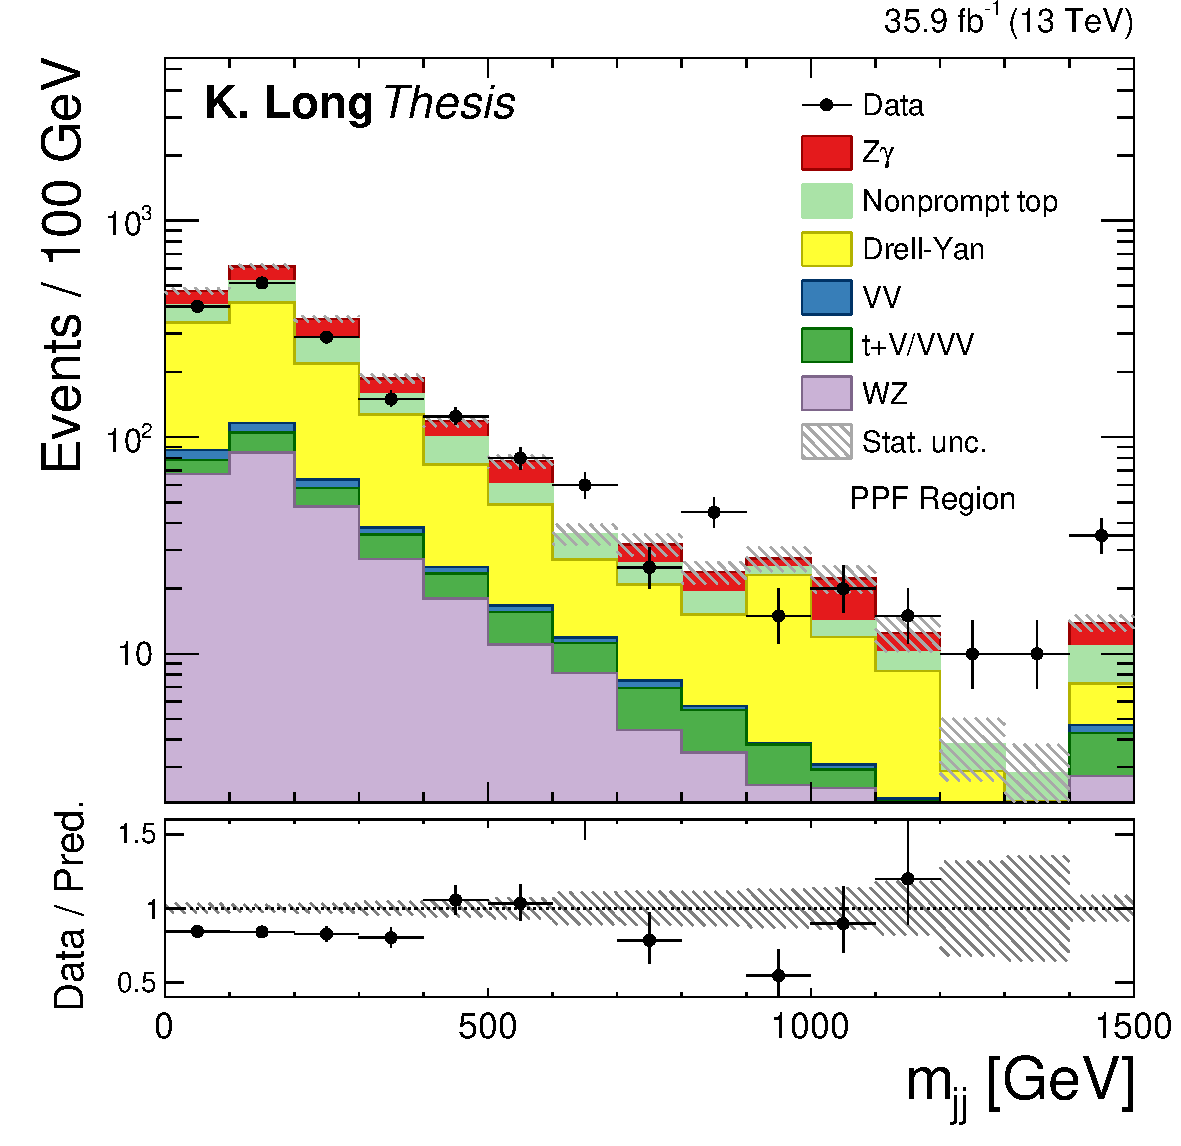
\includegraphics[width=0.45\textwidth]{figures/AnalysisProcedure/mjj_PPF.pdf}
   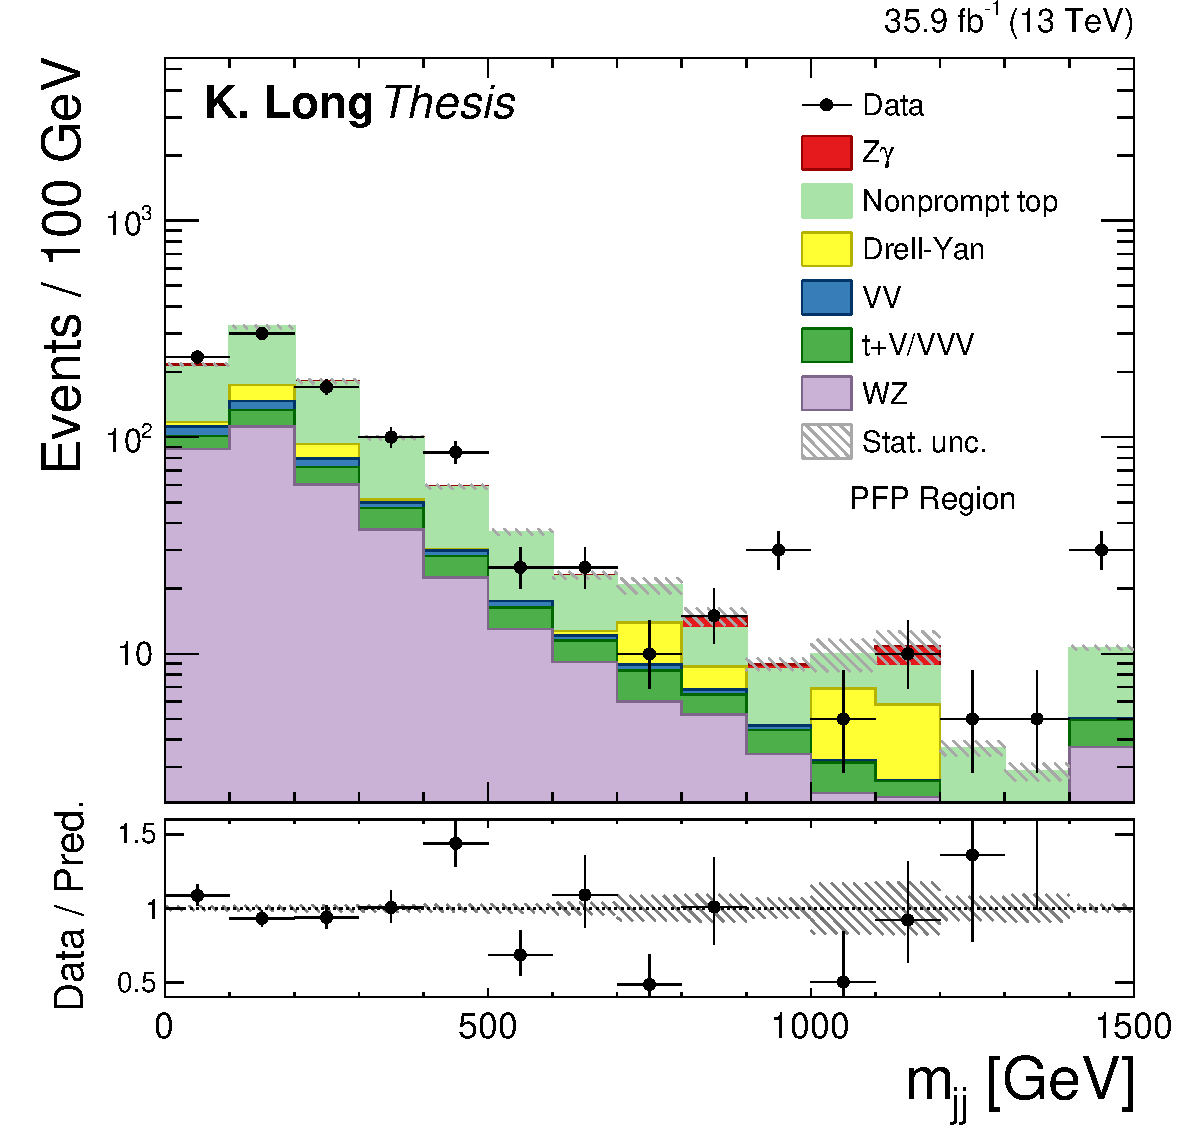
\includegraphics[width=0.45\textwidth]{figures/AnalysisProcedure/mjj_PFP.pdf}
  \caption[The PPF (left) and PFP (right) control regions used in the nonprompt estimation]{
    The PPF (left) and PFP (right) control regions used in the nonprompt estimation
    for events satisfying the \WZjj selection.
    The nonprompt MC simulations are shown for reference, and demonstrate that the
    PPF region is dominated by Drell--Yan events while the PFP region
    is dominated by {\ttbar} events.
        }
 \label{fig:nonpromptBackgroundCRs}
\end{figure}

A lepton candidate is labeled as ``passed'' (P) if it passes the ``tight'' identification
requirements required for signal events, 
and ``failed'' (F) if it passes the relaxed lepton identification criteria, 
but fails the tight identification. The signal region is defined by events 
with three passing leptons, referred to as PPP events. 
The loose lepton control regions are defined by the identification
criteria of the three selected lepton candidates. 
The PPF region, where the first
two labels refer to the two leptons which satisfy the tight identification criteria and are
associated with the \PZ boson candidate, and the failing lepton is associated with
the \cPW-candidate, is dominated by {\Zpj} events.
The $\mjj$ for the observed data compared to the prediction of the MC simulation
in the \WZjj selection, with $\pt^{\jet} > 30\GeV$, is shown in two illustrative control regions 
in Fig.~\ref{fig:nonpromptBackgroundCRs}. The nonprompt estimation does not depend on the 
nonprompt MC simulations, including Drell--Yan and $\ttbar$ production, which are shown for reference.
All possible combinations of P and F objects are listed in Table~\ref{tab:control_regions},
along with the dominant production mechanisms of such events.

\begin{table}[htbp]
    \centering
    \caption[Possible combinations of lepton identification for three-lepton events]{Possible combinations of lepton identification for three-lepton events
            that define the control regions used to estimate nonprompt backgrounds.}
    \begin{tabular}{c|ccc} 
\hline %------------------------------------------------------------------------------------------
Dominant        & \multicolumn{3}{c}{Combination}                                                  \\
contribution    & \multicolumn{2}{c}{Z-candidate leptons}   & W-candidate lepton                   \\
\hline %------------------------------------------------------------------------------------------
\hline %------------------------------------------------------------------------------------------
QCD multi-jet  & F & F & F \\ 
\hline %----------------------------------------------------------------------------------------- 
W+jets         & F & F & P \\
               & P & F & F \\
               & F & P & F \\
\hline %----------------------------------------------------------------------------------------- 
Z+jets         & P & P & F \\
\hline %----------------------------------------------------------------------------------------- 
\ttbar, other  & P & F & P \\
               & F & P & P \\
     \end{tabular}
    \label{tab:control_regions}
\end{table}

The expected contribution from these processes in the signal region is estimated
using ``loose-to-tight'' efficiency factors, which are
applied as extrapolation factors to the lepton candidates failing the analysis requirements 
in the control region events.
The efficiency factors, referred to as ``fake rates,'' are 
evaluated using samples of events dominated by jet activity.
A sample of $\PZ$+$\lcand$ events is defined by 
selecting events with exactly three leptons satisfying
the loose identification criteria, using the same trigger requirements as
for signal events.
Two opposite sign, same flavor 
leptons satisfying the tight identification and consistent with the decay of
a \PZ boson, specifically $\left|m_{\ell^{+}\ell^{-}} - m_\PZ\right| < 10\GeV$,
where $m_{\PZ}$ denotes the nominal \PZ boson mass, are required. To reduce contamination
from \WZ events, the events must additionally have $\ptmiss < 25\GeV$
and $m_{\rm T}(\ell_{3}, \ptmiss) < 25\GeV$. The lepton not associated with the 
\PZ boson candidate is taken as the {\lcand} object. 

\begin{figure}[htbp]
  \centering
   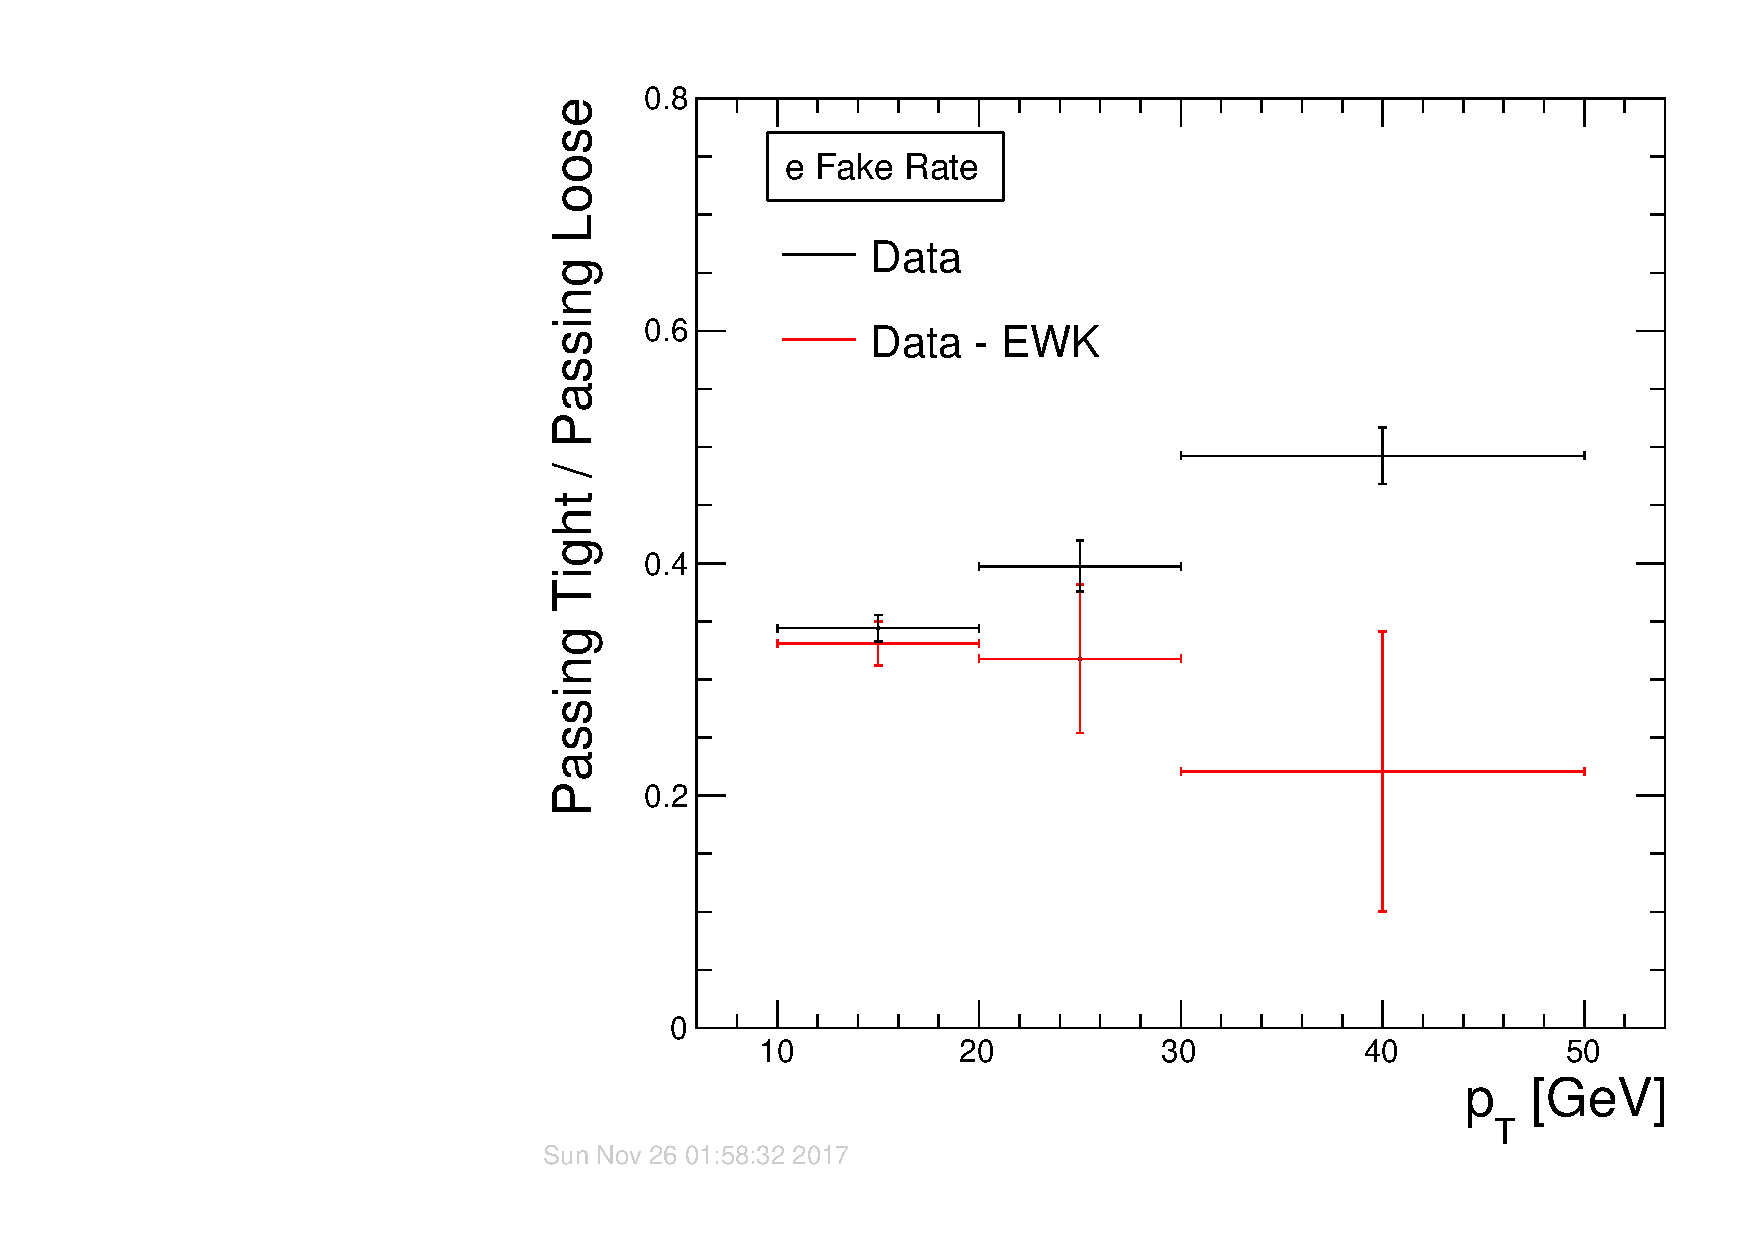
\includegraphics[width=0.4\textwidth]{figures/AnalysisProcedure/ratio1DPt_allE.pdf}
   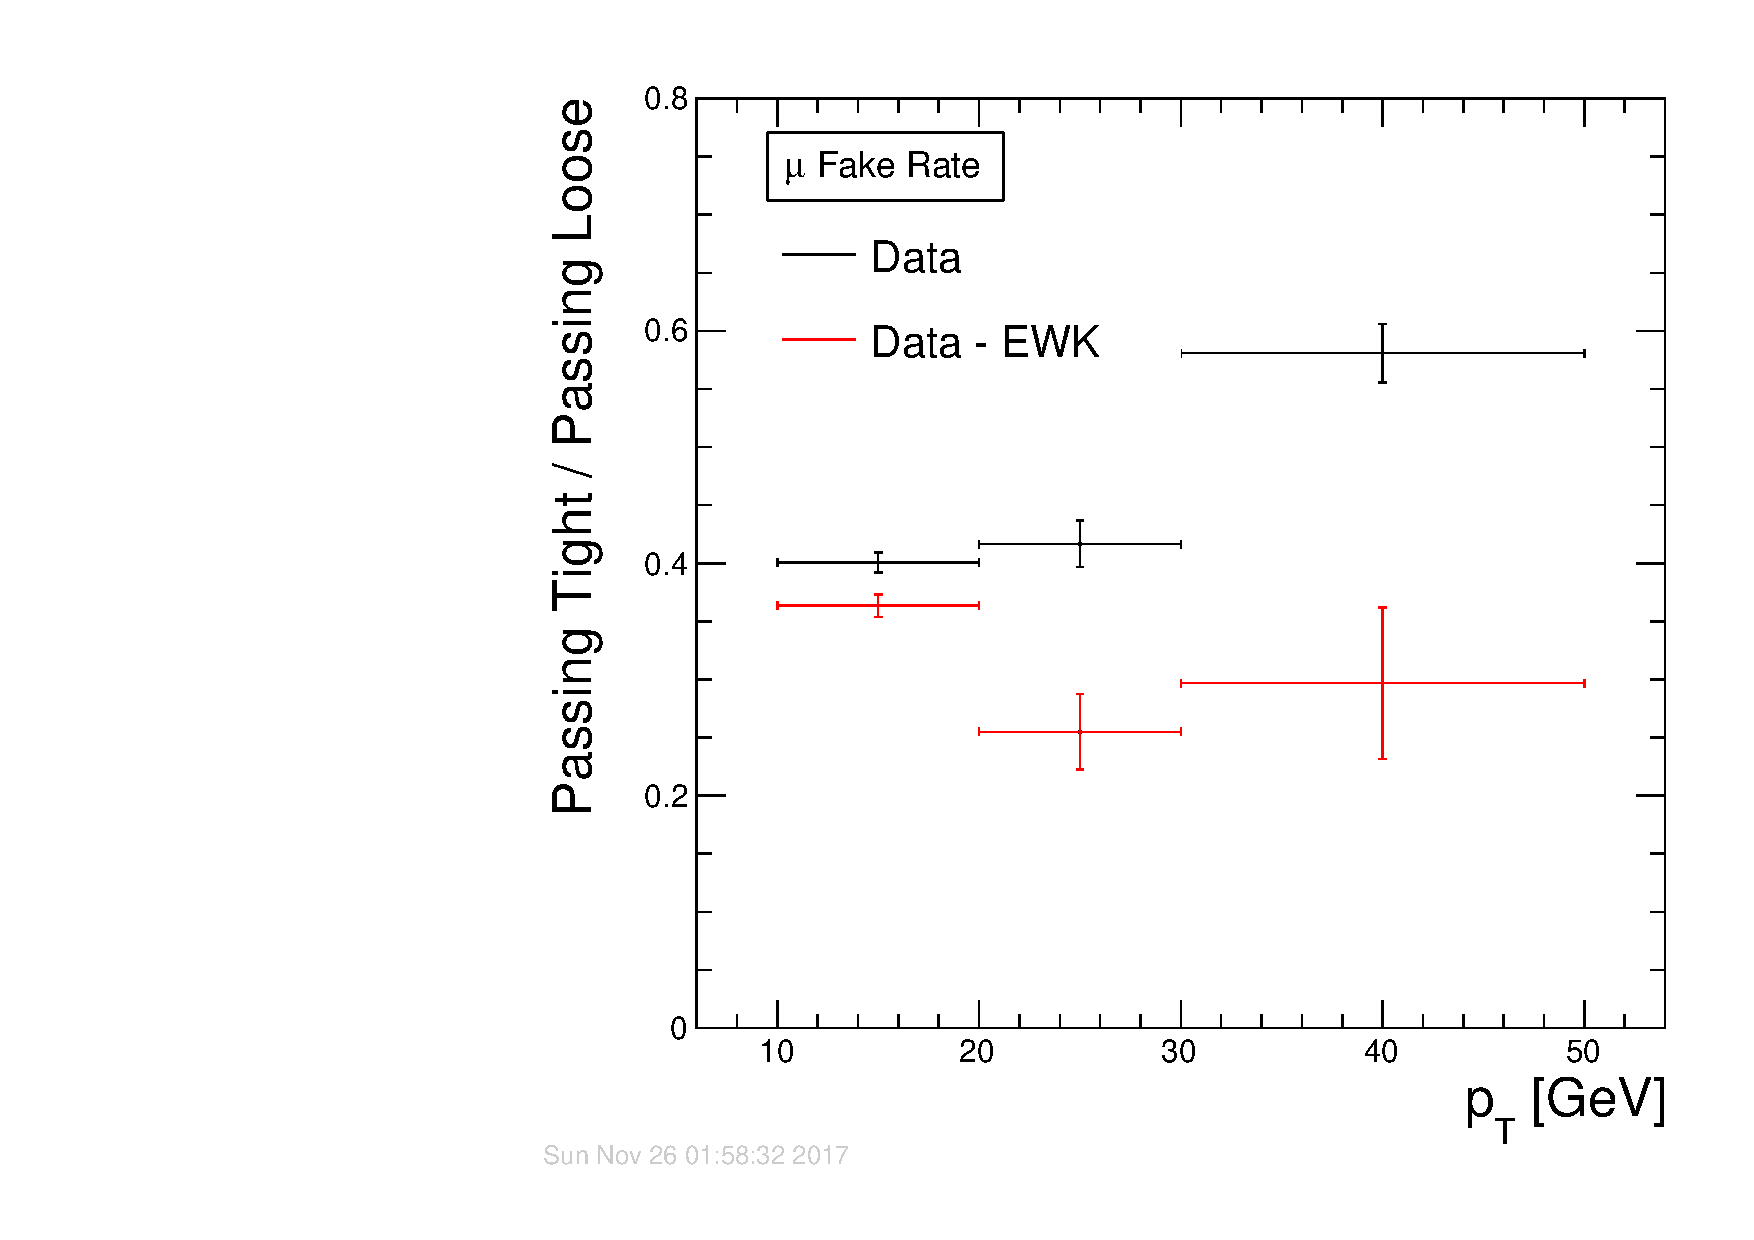
\includegraphics[width=0.4\textwidth]{figures/AnalysisProcedure/ratio1DPt_allMu.pdf}
   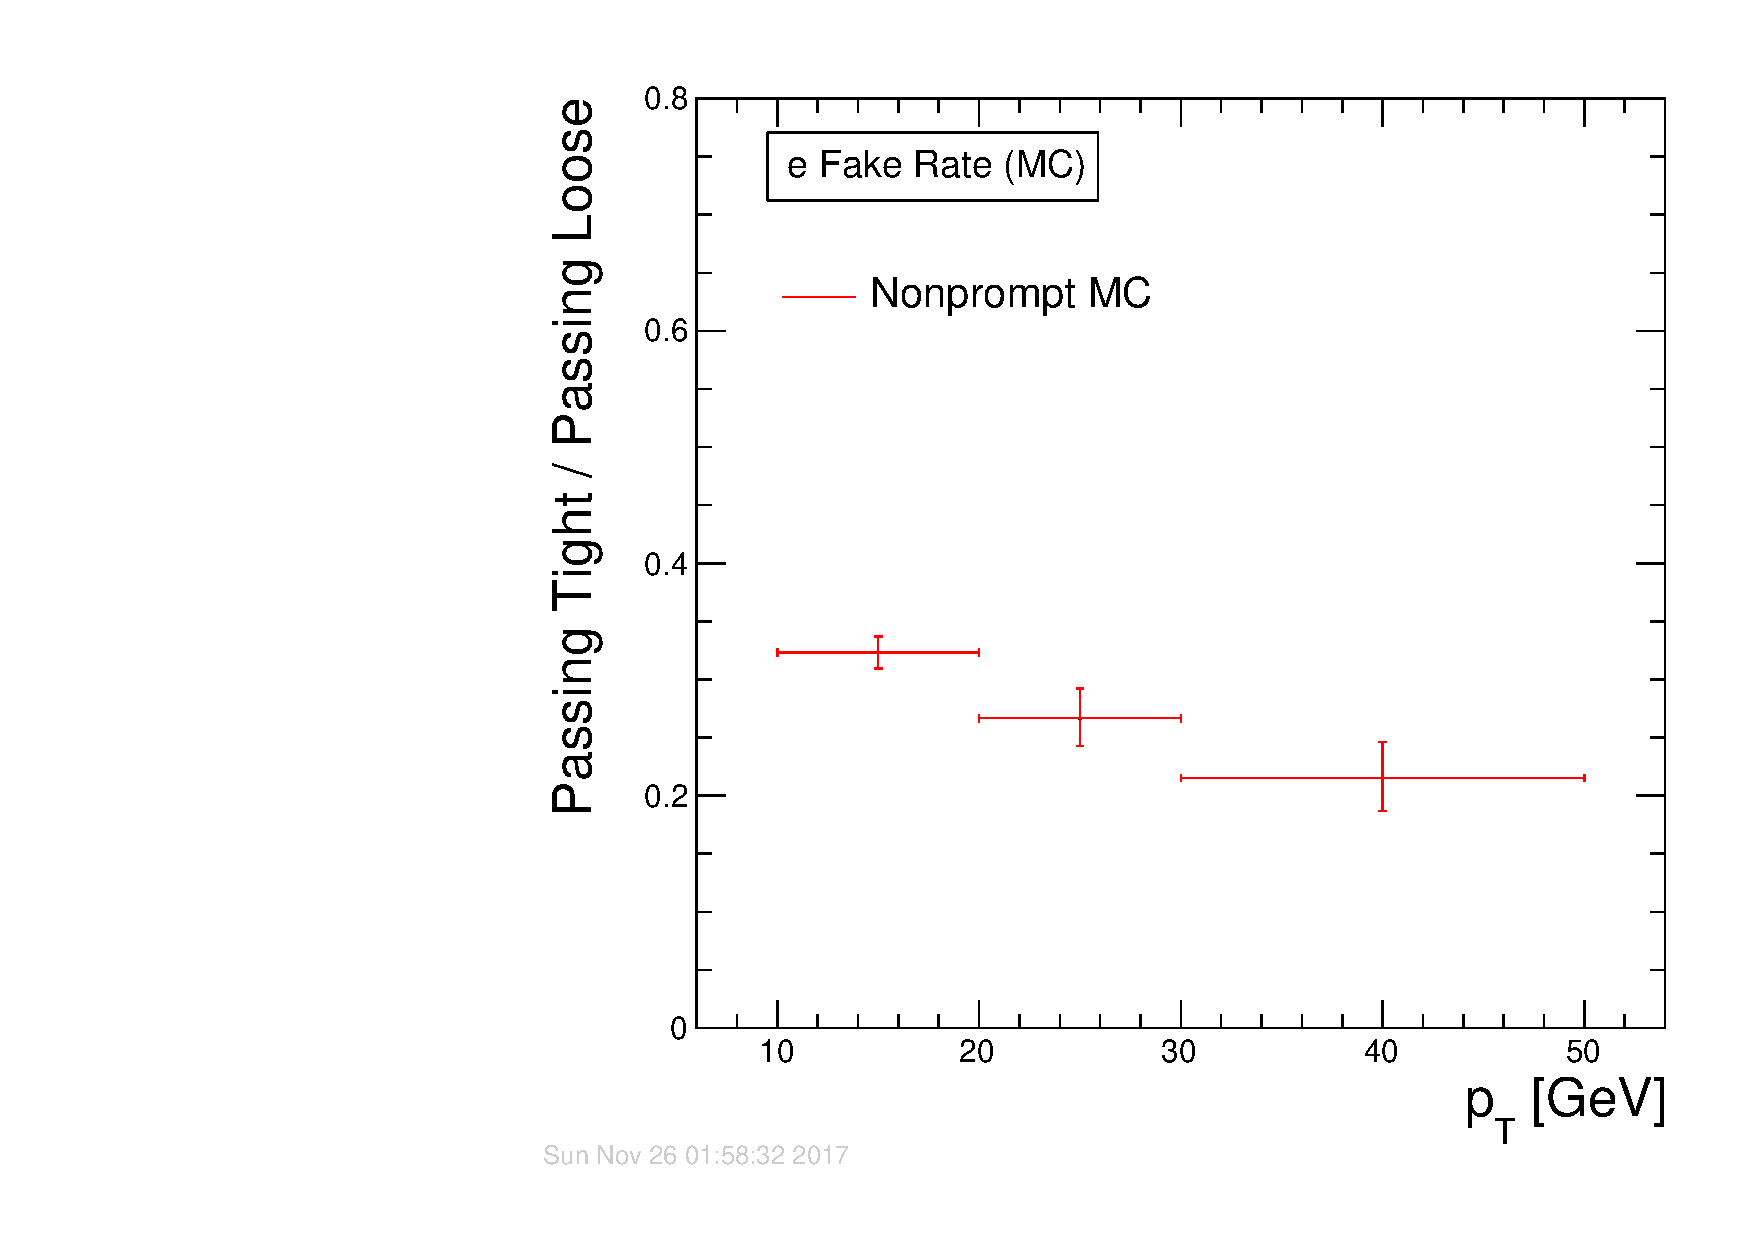
\includegraphics[width=0.4\textwidth]{figures/AnalysisProcedure/ratio1DPt_allE_MC.pdf}
   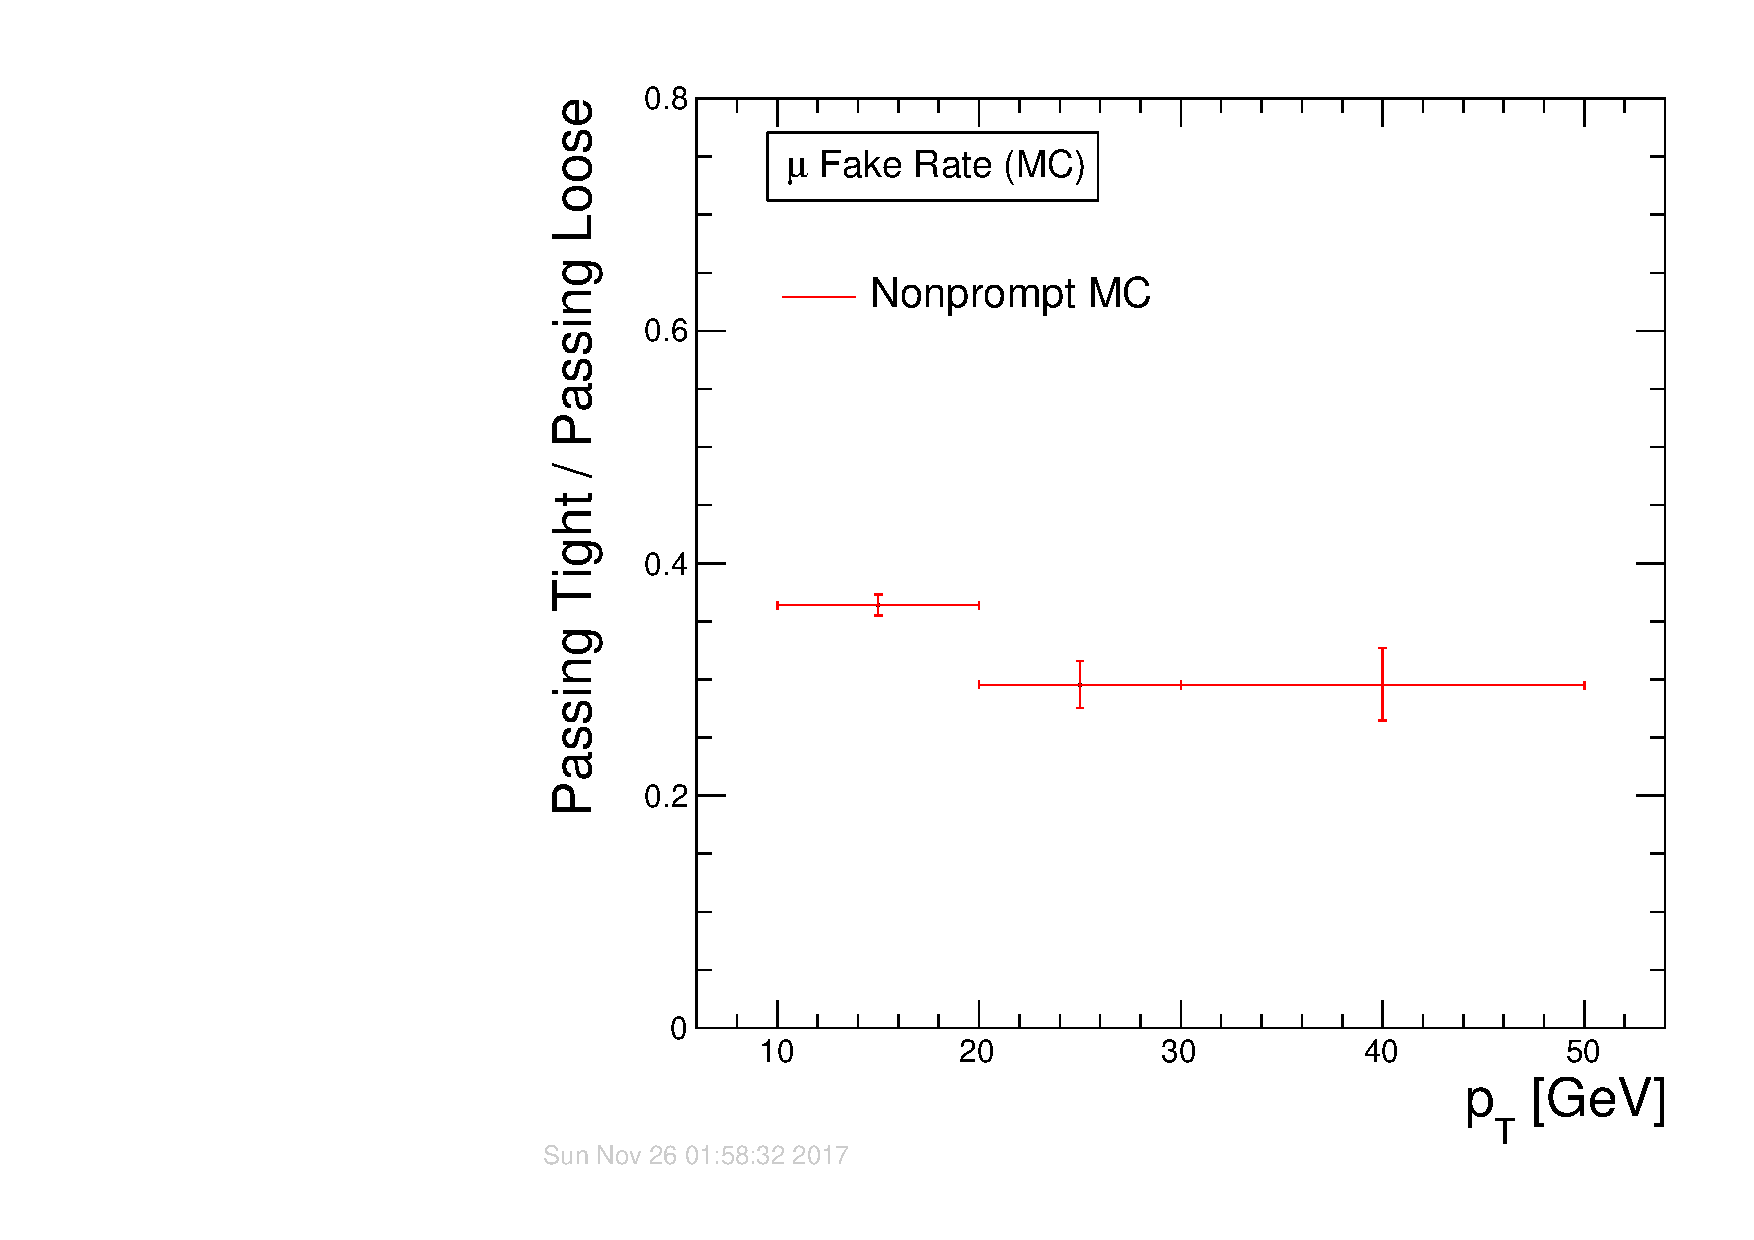
\includegraphics[width=0.4\textwidth]{figures/AnalysisProcedure/ratio1DPt_allMu_MC.pdf}
  \caption[Ratio of $\PZ+\ell_{\mathrm{candidate}}$ events passing the loose to events passing the tight idenification criteria]{
    Ratio of events in which the $\ell_{\rm candidate}$ objects passes the tight lepton 
    identification criteria to candidates passing only the loose lepton identification 
    criteria in bins of the {\lcand} \PT for the selection of $\PZ$+$\ell_{\mathrm{candidate}}$ 
    events described in the text.
    The events in which the $\ell_{\rm candidate}$ object is a electron (muon) are shown in 
    the left (right) plot. The top plots show events selected in data, with
    corrections for contamination of true prompt events from MC simulation. The bottom plots
    show predictions from the {\Zpj} and $\ttbar$ MC samples.
          }
 \label{fig:fakeRates1DPt}
\end{figure}

The fake rates are evaluated 
using ratios of events where the $\ell_{\mathrm{candidate}}$ 
object satisfies the full identification requirements 
to events where all identification criteria are not satisfied, defined as
$\varepsilon_{\text{fake}} = \frac{N_{\text{tight}}}{N_\text{loose}}$.
They are parameterized as a function of the {\lcand} \PT and $\eta$. 
The expected contribution from true three-prompt-lepton events is
estimated from MC simulation and subtracted from the event samples.
The fake rates measured in data, corrected using the prompt MC simulation,
and the predicted fake rates from the nonprompt MC simulation
are in good agreement, as shown in Fig.~\ref{fig:fakeRates1DPt}, 
The MC simulation prediction is not used in the analysis, but serves as a consistency-check
of the nonprompt estimation technique.
The two-dimensional values of the fake rates derived from data which are used for
the analysis are shown in Fig.~\ref{fig:fakeRates2D}.

\begin{figure}[htbp]
  \centering
   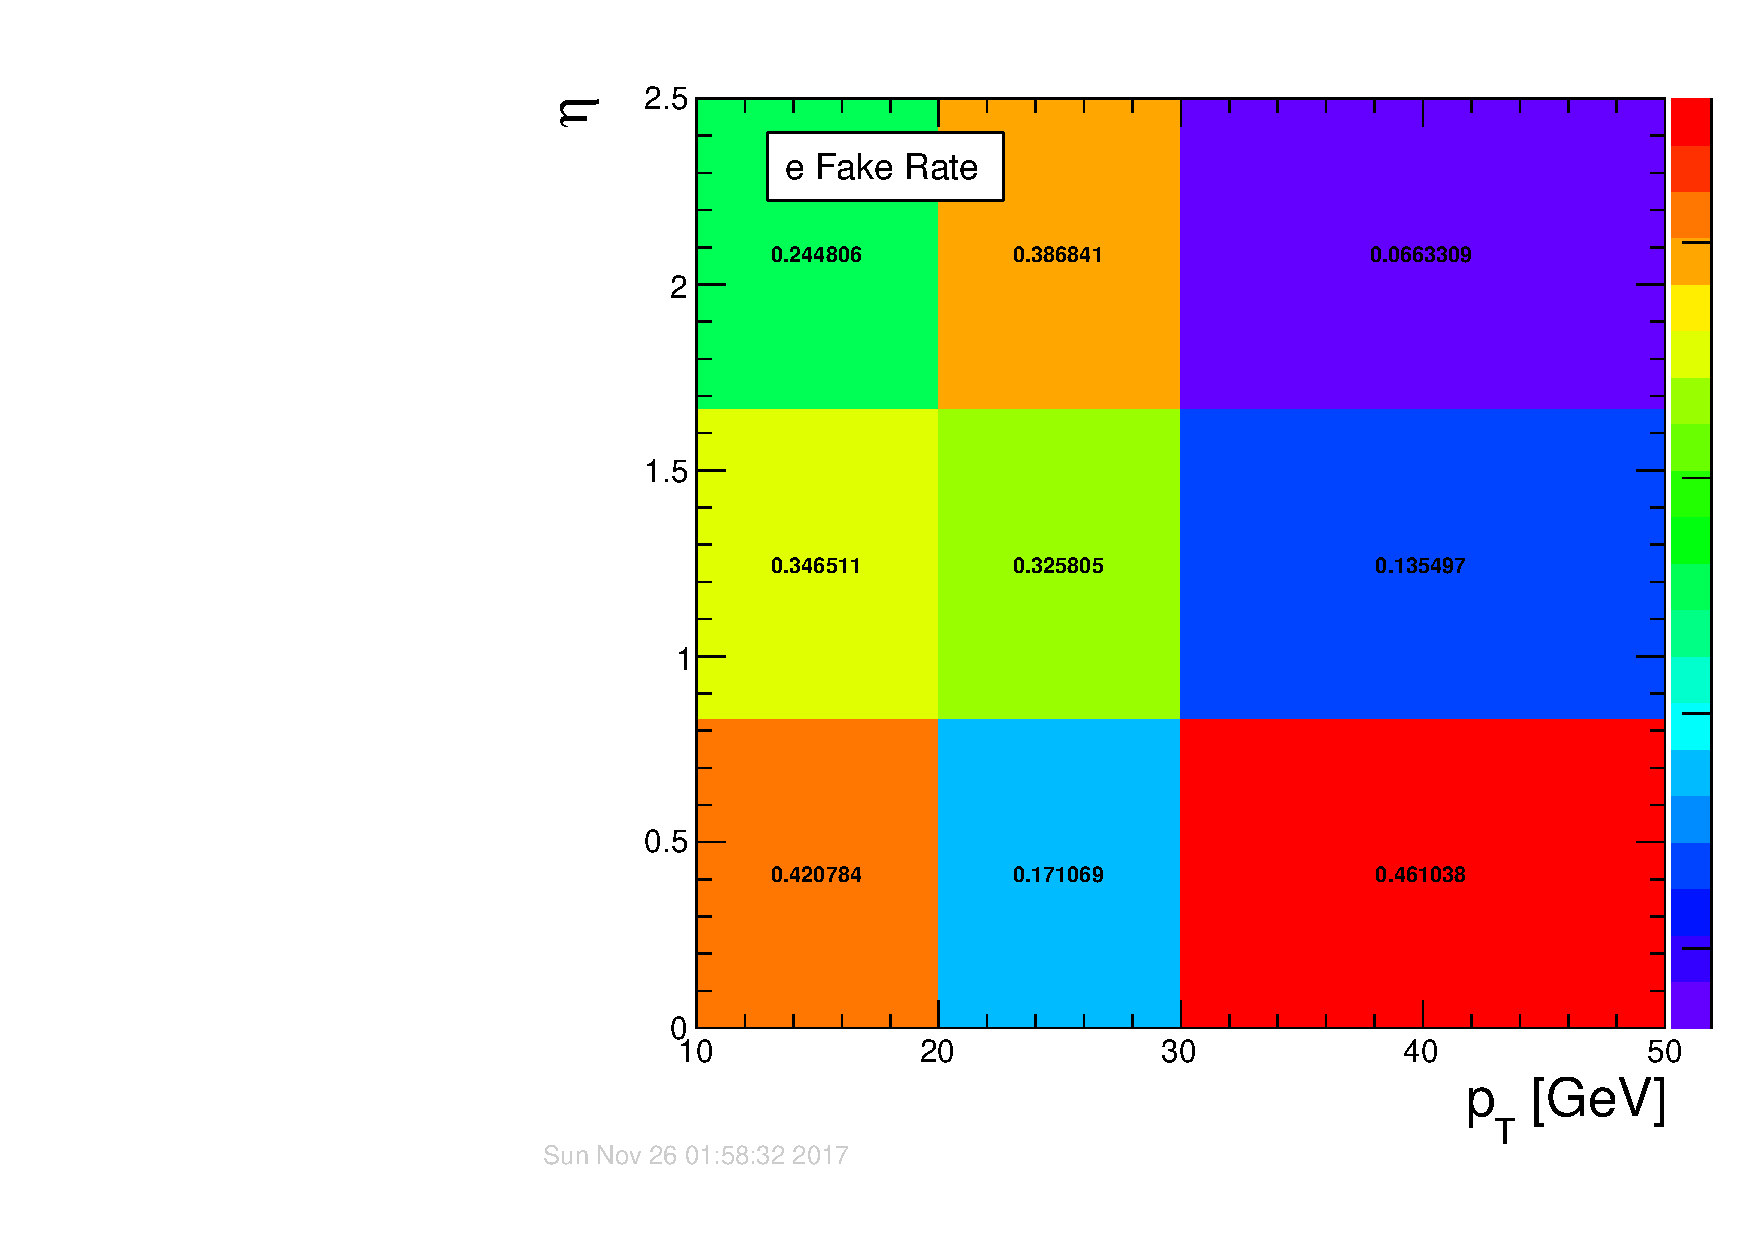
\includegraphics[width=0.45\textwidth]{figures/AnalysisProcedure/ratio2D_allE.pdf}
   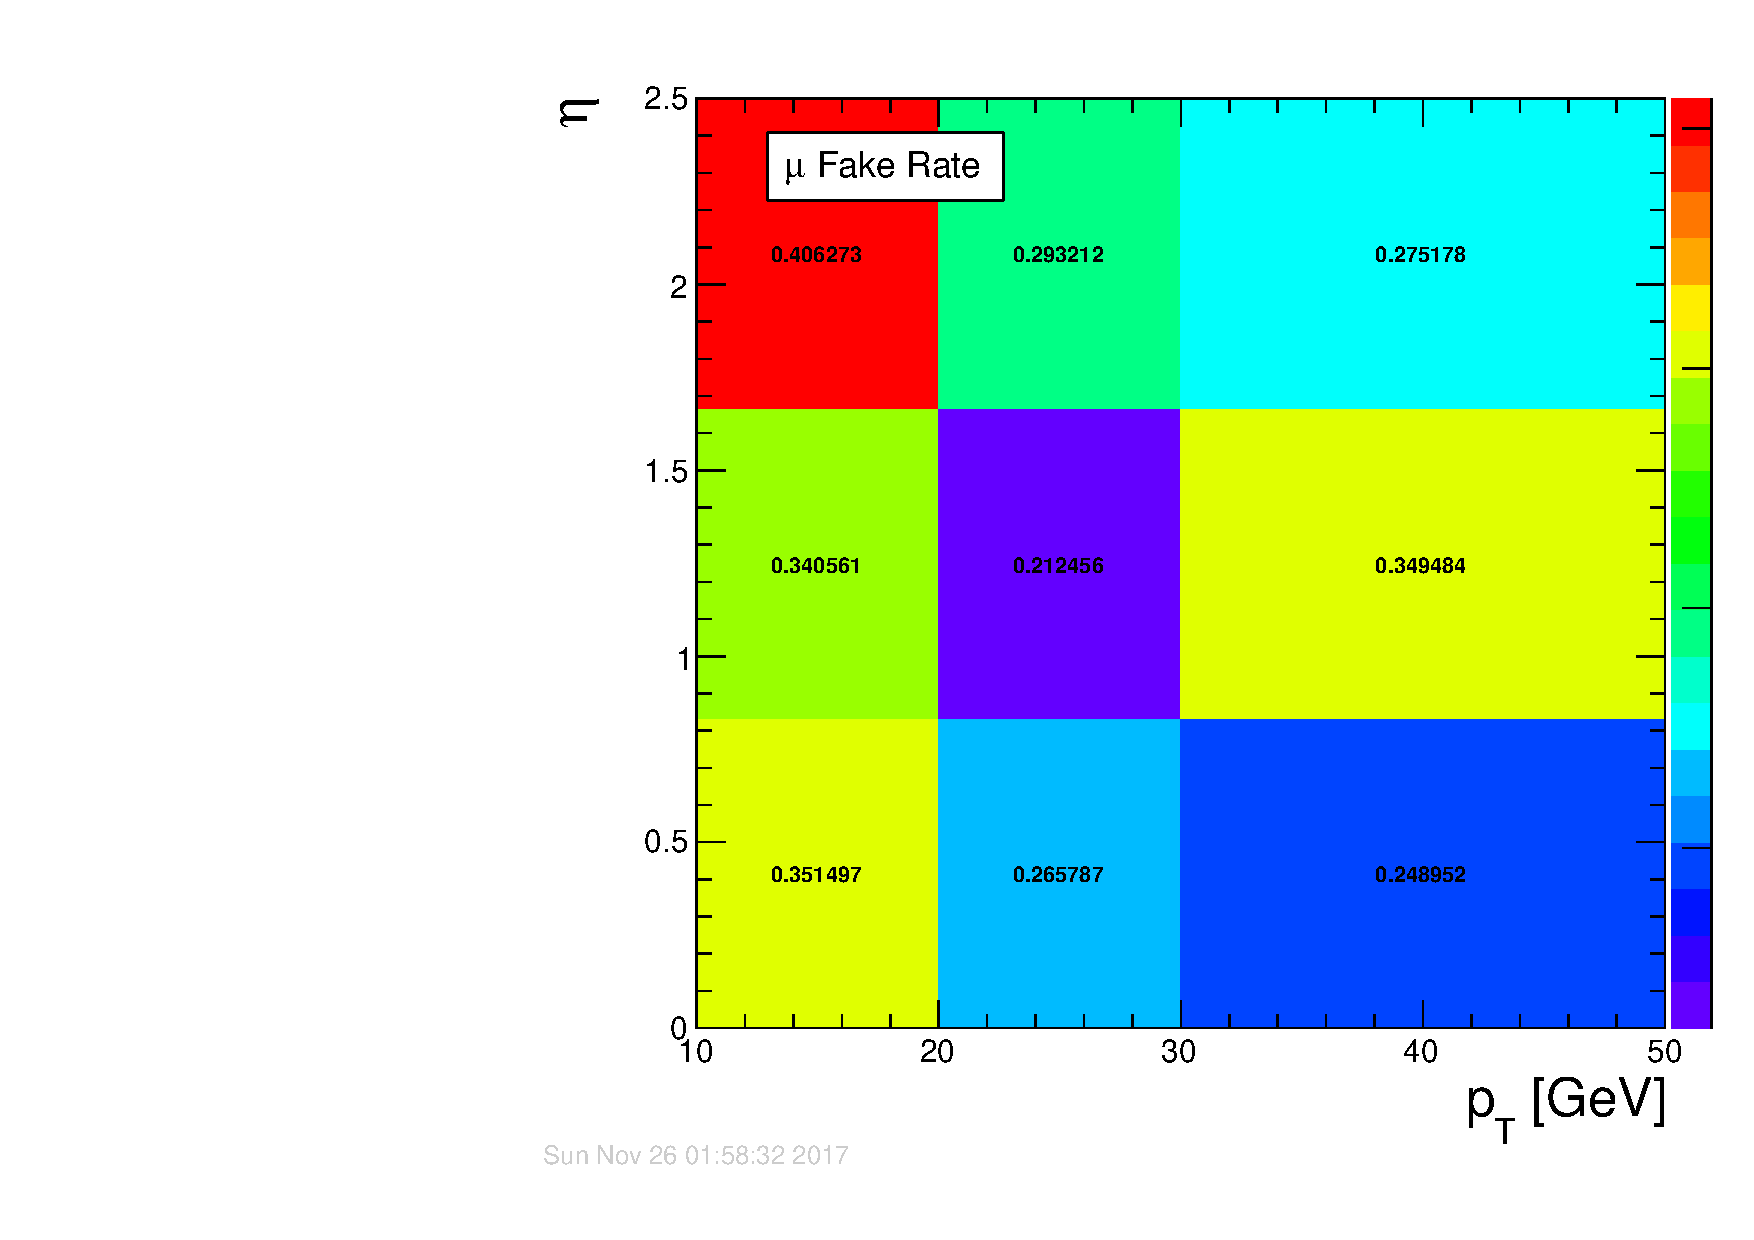
\includegraphics[width=0.45\textwidth]{figures/AnalysisProcedure/ratio2D_allMu.pdf}
  \caption[Two-dimensional ratios of $\PZ+\ell_{\mathrm{candidate}}$ events passing the loose to events passing the tight idenification criteria]{
    Ratio of events in data, with corrections for contamination of true prompt events from MC simulation,
    in which the $\ell_{\rm candidate}$ objects passes the tight lepton 
    identification criteria to candidates passing only the loose lepton identification 
    criteria in bins of \PT and $\eta$ for the selection of $\PZ$+$\ell_{\mathrm{candidate}}$ 
    events described in the text.
    The events in which the $\ell_{\rm candidate}$ object is a electron (muon) are shown in 
    the left and right plots respectively. 
        }
 \label{fig:fakeRates2D}
\end{figure}


A cross-check of the technique is performed by 
repeating the procedure with efficiency factors derived from a 
sample of events dominated by dijet production. 
Events passing single lepton triggers are selected, requiring at least one jet and one
{\lcand} object passing the loose identification. Events with additional loose leptons are not selected.
The loose lepton must be separated from the jet with highest \pt by $\Delta R(\lcand, \jet) > 1$.
The contamination of WZ is suppressed by requiring $E_T^{\text{miss}} < 25\,\GeV$  and  $m_T < 25\,\GeV$. 
The loose-to-tight efficiency factors obtained in the two regions
agree to within 30\% for the full \PT and $\eta$ range.

\begin{table}[htbp]
    \centering
    \begin{tabular}{|c|c|c|c|c|c|c|c| }
\hline %------------------------------------------------------------------------------------------ 
Control region &  \multicolumn{7}{c|}{Includes regions}                                                                 \\
\hline %------------------------------------------------------------------------------------------ 
FPP & FPP &     &     & FFF & FPF & FFP &        \\
PFP &     &     & PFP & FFF &     & FFP & PFF    \\
PPF &     & PPF &     & FFF & FPF &     & PFF    \\
FPF &     &     &     & FFF & FPF &     &        \\
FFP &     &     &     & FFF &     & FFP &        \\
PFF &     &     &     & FFF &     &     & PFF    \\
FFF &     &     &     & FFF &     &     &        \\
\hline %------------------------------------------------------------------------------------------ 
     \end{tabular}
    \caption{ Possible nonprompt control regions and regions of overlap.}
    \label{tab:nonpromptRegionOverlap}
\end{table}

Because control regions with $n_{F}$ failing leptons can contribute to the region with
$n_{F}-1$ failing leptons,
the total background contribution in the signal region is not a simple sum of the 
loose lepton control region event yields multiplied by the fake rate of each failing leptons. 
Table~\ref{tab:nonpromptRegionOverlap} shows the possible contributions 
of loose lepton control regions with loose leptons into tight lepton regions.
For example,
the estimated contribution of events to the signal region $N_{B,FPP+PFP}$ 
from the FPP and PFP loose lepton control regions, with $N_{FPP}$ and $N_{PFP}$ data events is given by

\begin{multline*}
N_{B,FPP + PFP} = N_{FPP} \times f_{l1}
  - \underbrace{N_{FFF} \times f_{11} \times f_{l2} \times f_{l3}}_{\textrm{interference of FPP and FFF}} \\
  - \underbrace{f_{l1} \times f_{l3} \times (N_{FPF} - N_{FFF} \times f_{l2} )}_{\textrm{interference of FPP and FPF}}
- \underbrace{f_{l1} \times f_{l2} \times (N_{FFP} - N_{FFF} \times f_{l3})}_{\textrm{interference of FPP and FFP}}\\
 + N_{PFP} \times f_{l2} -  \underbrace{N_{FFF} \times f_{11} \times f_{l2} \times f_{l3}}_{\textrm{interference of PFP and FFF}}
 - \underbrace{f_{l1} \times f_{l2} \times (N_{FFP} - N_{FFF}  \times f_{l3})}_{\textrm{interference of PFP and FFP}}\\
  - \underbrace{f_{l2} \times f_{l3} \times (N_{PFF} -  N_{FFF} \times f_{11} )}_{\textrm{interference of PFP and PFF}} = \\
  N_{FPP} \times f_{l1} +  N_{PFP} \times f_{l2} - 2 N_{FFF} \times f_{11} \times f_{l2} \times f_{l3}
   - 2 N_{FFP} \times f_{l1} \times f_{l2} \\ - N_{FPF} \times f_{l1} \times f_{l3} -  N_{PFF} \times f_{l2} \times f_{l3}
\end{multline*}

where $f_{l1} = \frac{\varepsilon_{\text{fake}}}{1 - \varepsilon_{\text{fake}}}$, 
computed from the misidentification ratio $\varepsilon_{\text{fake}}$ in the 
particular $p_{\text{T}}$ and $\eta$ bin.

Combining the yields from all seven loose lepton control regions in this way yields the following formula
for the total number of estimated background events from all regions 

\begin{align*}
N_B = N_{FPP} \times FR_{l1} + N_{PFP} \times FR_{l2} + N_{PPF} \times FR_{13} 
 + N_{FFF} \times FR_{11} \times FR_{l2} \times FR_{l3}  \\
- N_{FPF} \times FR_{l1} \times FR_{l3} - N_{FFP} \times FR_{l1} \times FR_{l2} - N_{PFF} \times FR_{l2} \times FR_{l3} \,.
\label{eqn:fakerate}
\end{align*}

The characteristics of the control region events
are used to obtain per-channel differential predictions in the signal region.
The expected contribution of nonprompt events in the signal region is shown
in Fig.~\ref{fig:expectedEWSignal}, where the signal and background 
normalizations are fixed to their expected
values and the expected sum of signal and background events is treated as the 
observed data.

This method is validated in nonoverlapping data samples enriched in Drell--Yan and $\ttbar$ contributions.
The Drell--Yan region is defined by inverting the selection requirement in $\ptmiss$, and
the $\ttbar$ region is defined by requiring at least one b-tagged jet and rejecting events with $|m_{\ell'\ell'} - m_\PZ| < 5\GeV$
while keeping all other requirements for the signal region.
The background prediction and observed data in these regions for events statisfying the {\WZjj} selection are shown in
Fig.~\ref{fig:nonpromptValidationRegions}, which demonstrates agreement between the two techiques.
The predictions for large values of $\mjj$ and
$\etajj$ are limited by the event count of data events used for the nonprompt esitmation.

\begin{figure}[htbp]
  \centering
   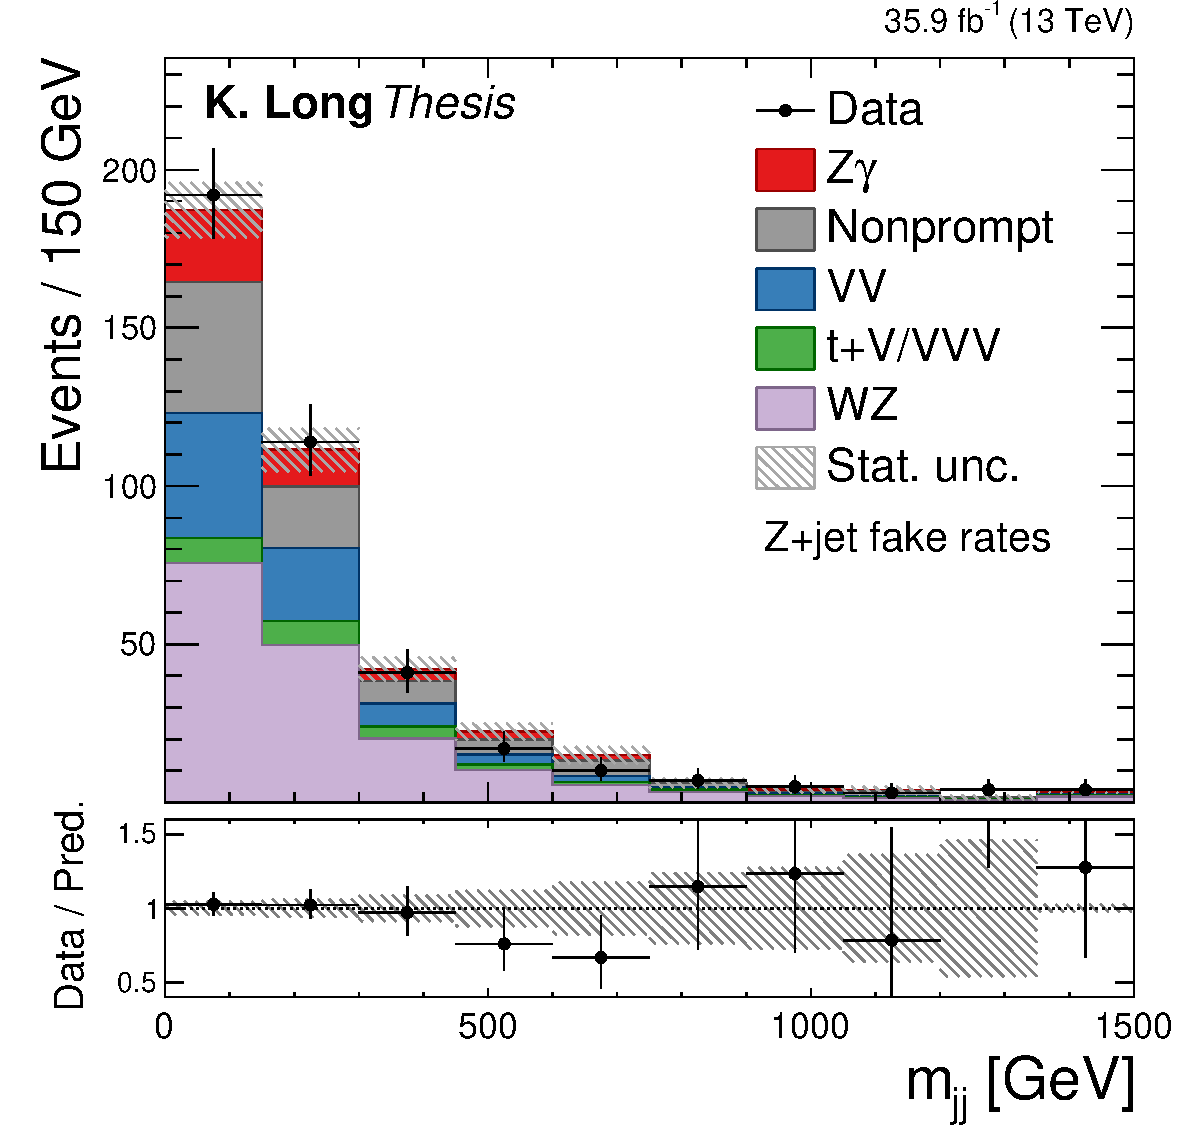
\includegraphics[width=0.4\textwidth]{figures/AnalysisProcedure/mjj_3lDYControl.pdf}
   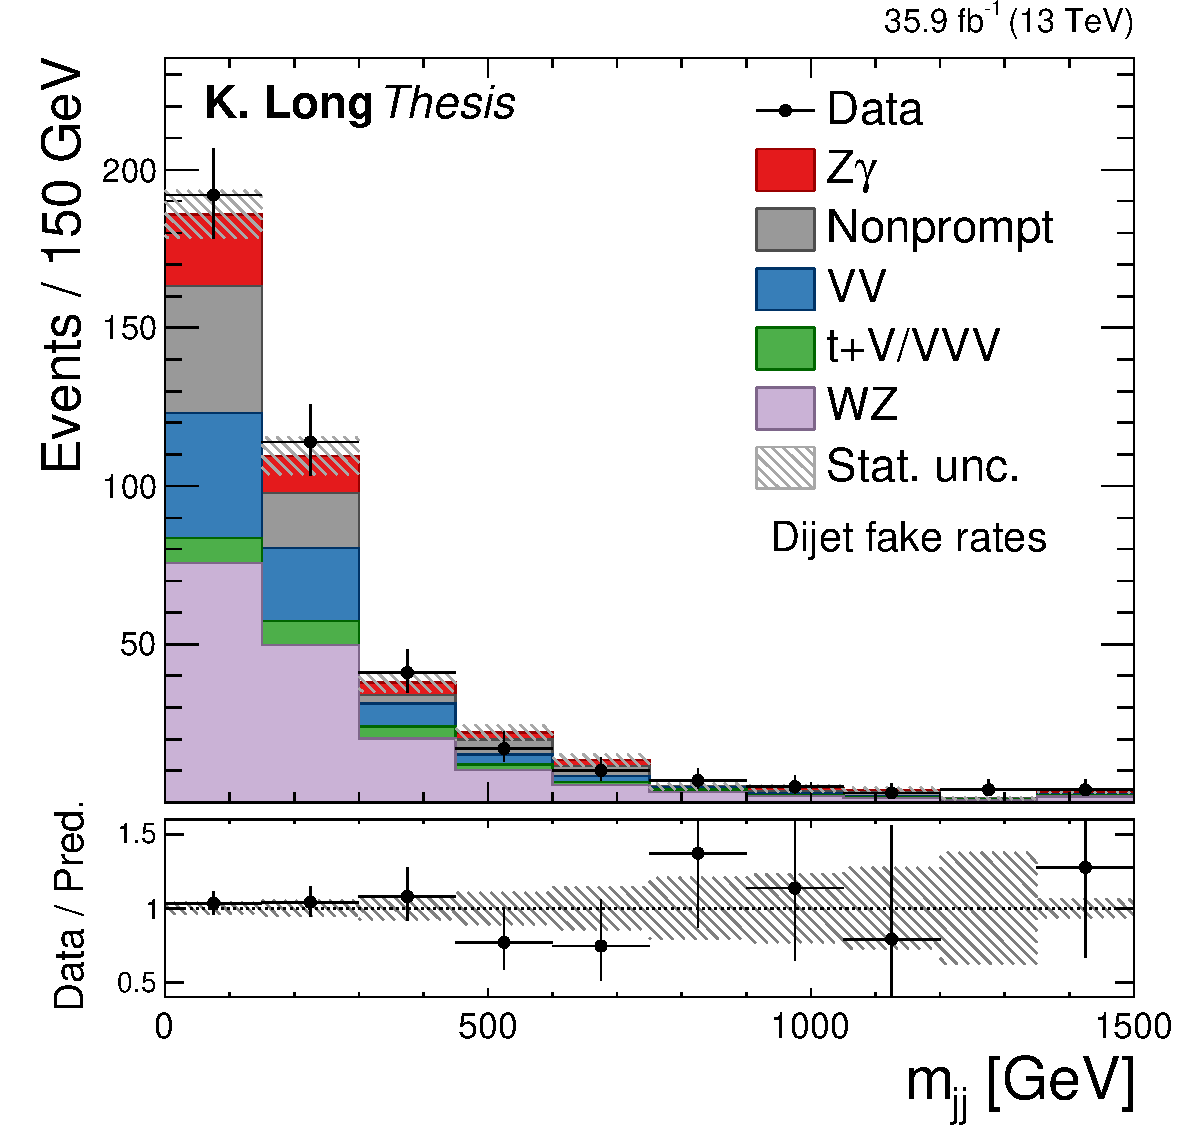
\includegraphics[width=0.4\textwidth]{figures/AnalysisProcedure/mjj_3lDYControl_dijetFRs.pdf}
   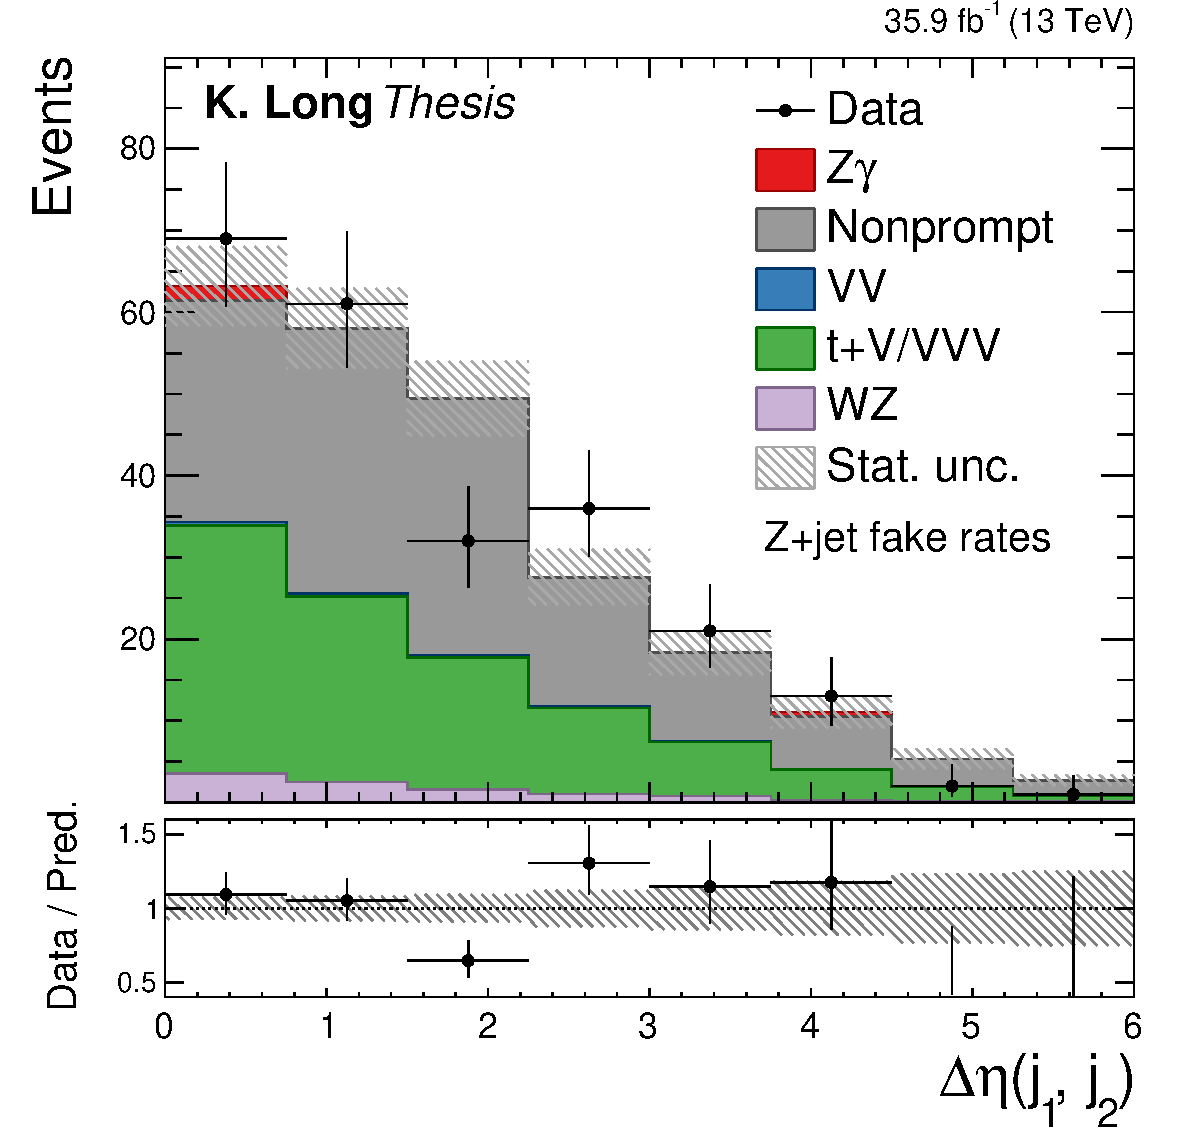
\includegraphics[width=0.4\textwidth]{figures/AnalysisProcedure/dEtajj_3lTTbarControl.pdf}
   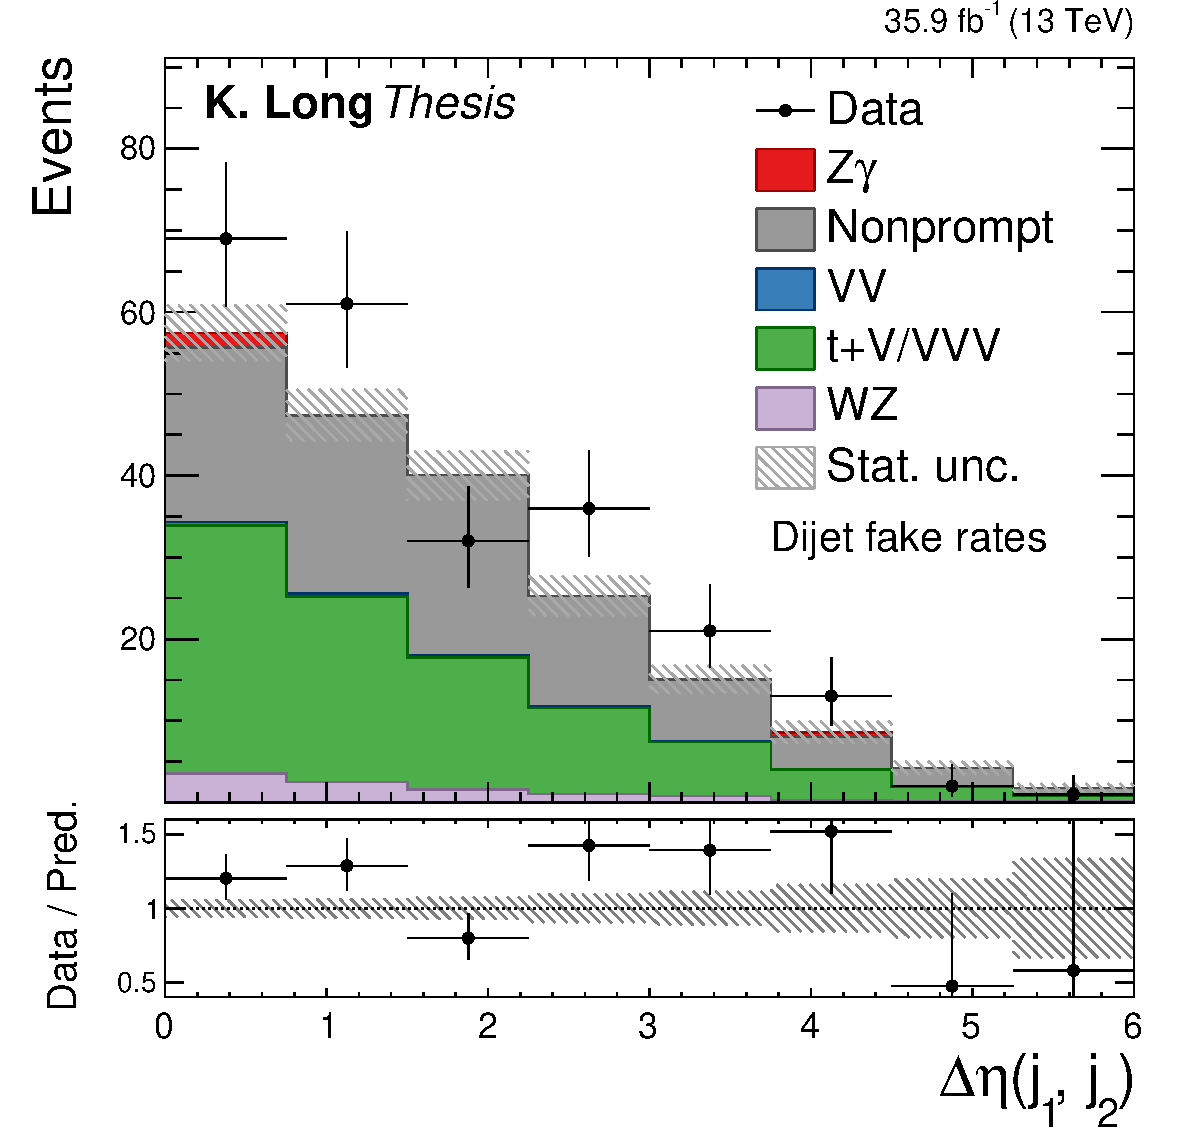
\includegraphics[width=0.4\textwidth]{figures/AnalysisProcedure/dEtajj_3lTTbarControl_dijetFRs.pdf}
  \caption[$\mjj$ and $\etajj$ for events in the Drell--Yan and $\ttbar$ control regions]{
    $\mjj$ for events in the Drell--Yan control region (top)
    and $\etajj$ for events in the $\ttbar$ control region (bottom).
    The events are required to have two $\pt > 30\GeV$
    jets but no additional kinematic selection is applied to the dijet system.
        }
 \label{fig:nonpromptValidationRegions}
\end{figure}

The event count of the loose lepton control samples of nonprompt events
satisfying the EW signal selection severely limits
differential predictions in this region. This is illustrated in 
Fig.~\ref{fig:nonpromptdEtajjByChan}, which shows the differential
prediction from the nonprompt background in the EW signal region,
which is particularly limited when dividing distributions by decay channel.

\begin{figure}[htbp]
  \centering
   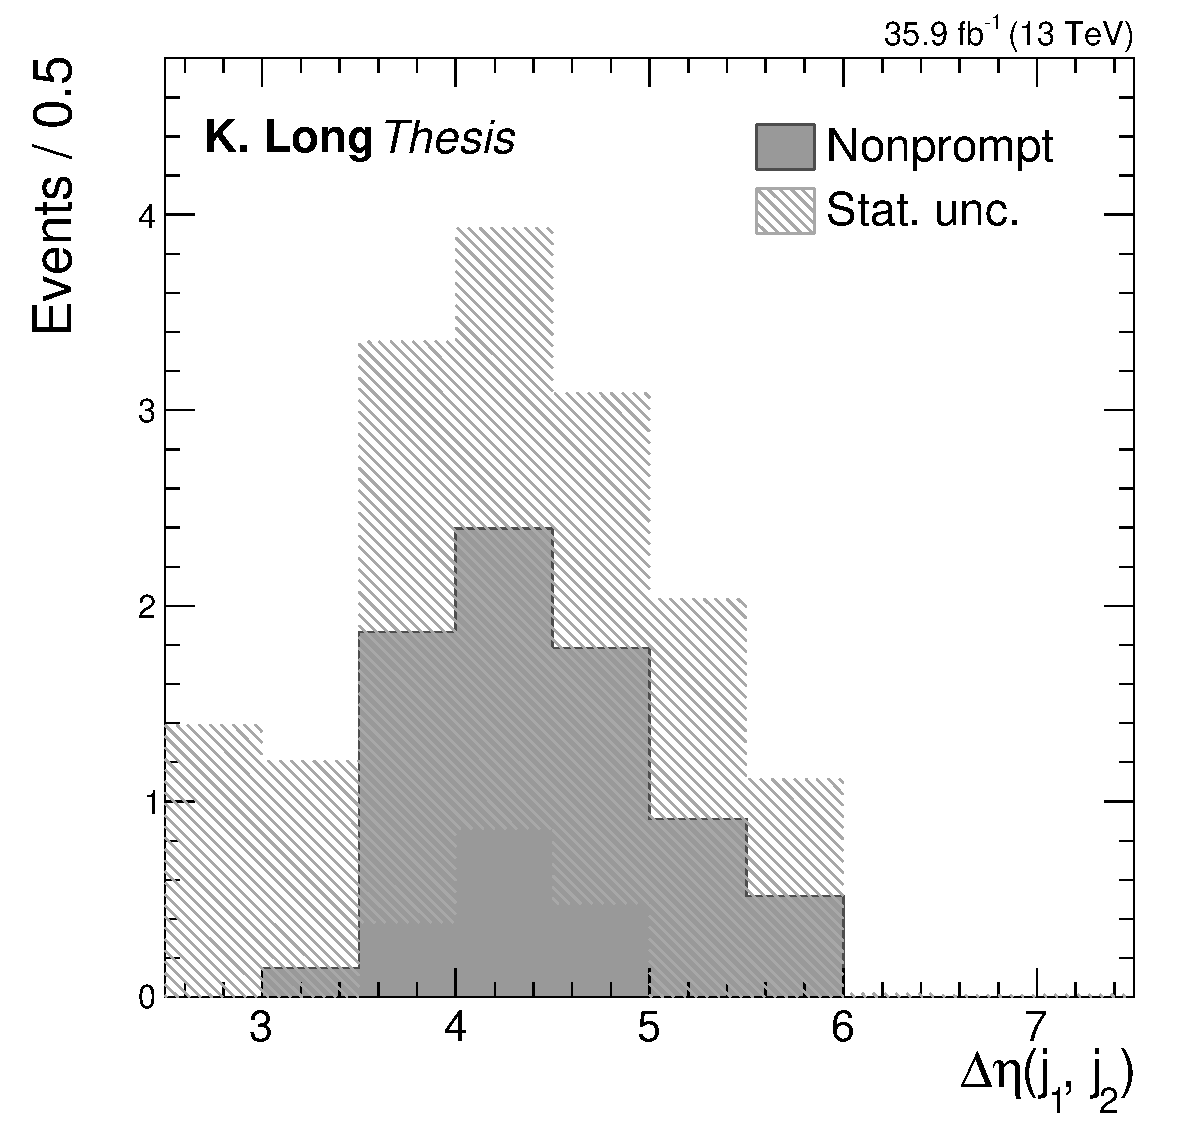
\includegraphics[width=0.4\textwidth]{figures/AnalysisProcedure/dEtajj_nonprompt.pdf}
   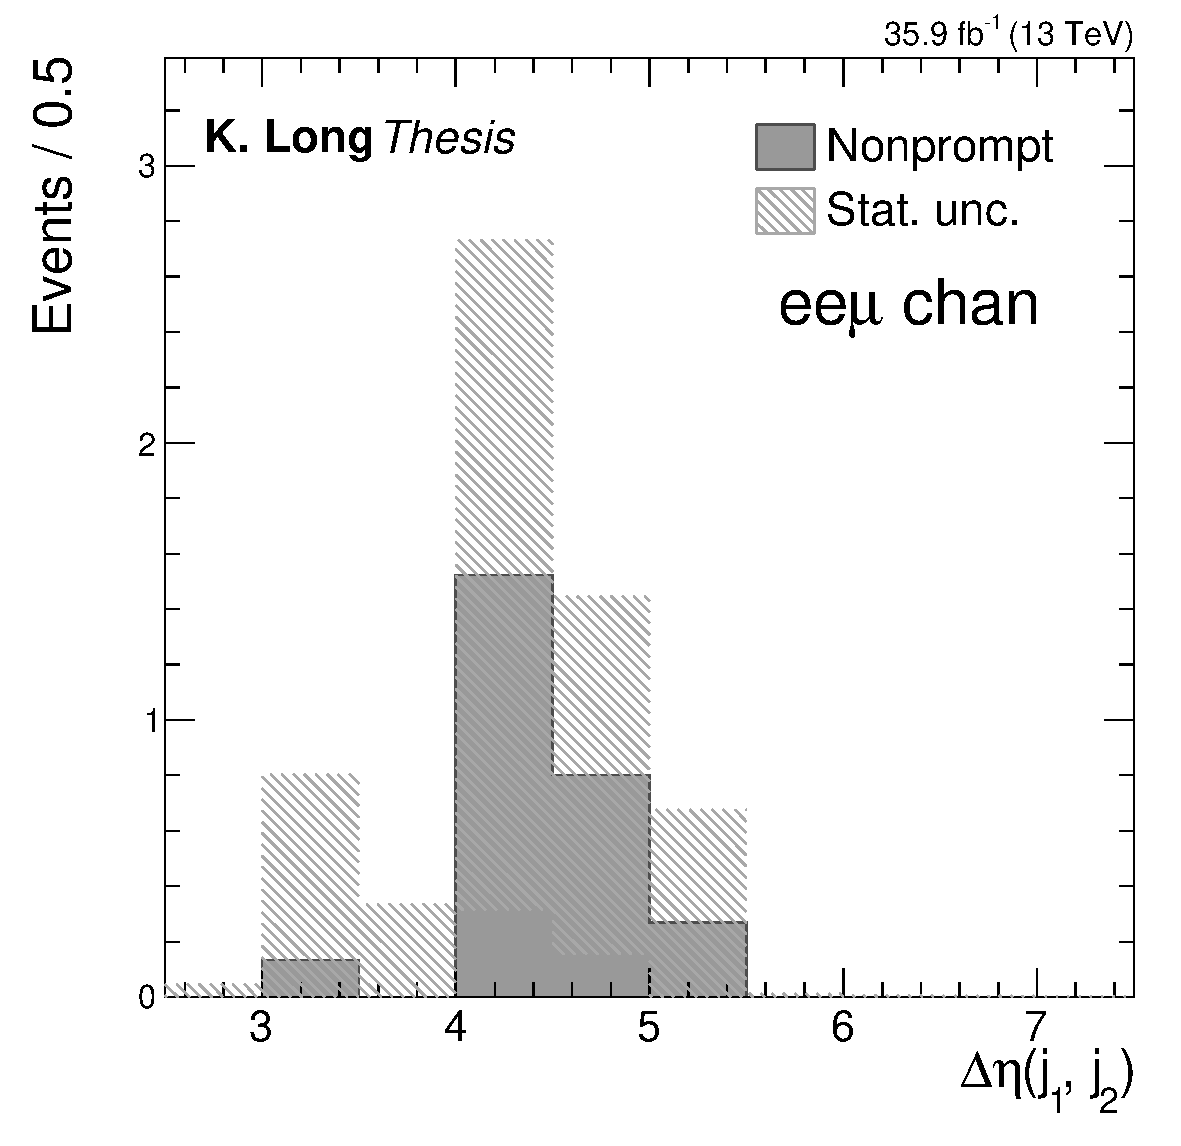
\includegraphics[width=0.4\textwidth]{figures/AnalysisProcedure/dEtajj_nonprompt_eem.pdf}
  \caption[Distribution of $\etajj$ for estimated nonprompt events in the \EW signal region]{
    Distribution of $\etajj$ for estimated nonprompt events in the EW signal region. The
    left plot shows the combined contribution for all channels, while the right plot shows
    the contribution from only the ee$\mu$ channel, which is severally limited by the 
    event count in the loose lepton control samples. 
        }
 \label{fig:nonpromptdEtajjByChan}
\end{figure}

The combined shape of the nonprompt background for all channels 
is therefore used for each channel in the \EWWZ 
measurement and in the extraction of constraints on anomalous quartic
gauge couplings. 
The normalization of the distribution per channel is taken from the 
ratio of the nonprompt yield in a single channel to the total nonprompt event yield 
measured in \WZjj events with no requirements on the dijet system.
These ratios are found to be consistent within the statistical uncertainty with ratios measured
when relaxing the jet \PT requirement in \WZjj events, in \WZ events inclusive in the number of jets, 
and in events satisfying the EW signal and control region selections, as demonstrated in
Table~\ref{tab:nonpromptNorms}.


\begin{table}[htbp]
     \centering
     \caption{
       Relative fraction of nonprompt events by channel for different selections of \WZ and \WZjj events.
           }
     \begin{tabular}{l|cccc}
 \hline %------------------------------------------------------------------------------------------
       Selection           &   \eee           & \eem             &   \emm         &   \mmm  \\	
 \hline %------------------------------------------------------------------------------------------
 \hline %------------------------------------------------------------------------------------------
       \WZ inclusive       & $ 0.06 \pm 0.04$	& $0.18 \pm 0.03$  & $0.21 \pm 0.04	$ & $0.55 \pm 0.04$ \\
       \WZjj               & $ 0.08 \pm 0.05$	& $0.16 \pm 0.05$  & $0.33 \pm 0.07	$ & $0.44 \pm 0.06$ \\
       Charged Higgs boson & $ 0.14 \pm 0.14$	& $0.22 \pm 0.14$  & $0.30 \pm 0.21	$ & $0.34 \pm 0.15$ \\
        EW signal          & $< 0.1 \pm 0.1 $	& $0.23 \pm 0.19$  & $0.57 \pm 0.34 $	& $0.21 \pm 0.16$ \\
  \hline
  \end{tabular}
  \label{tab:nonpromptNorms}
\end{table}

\section{Statistical proceduress}
\label{sec:statistics}

The distribution of data events in a quantum process is fundamentally stochastic 
in nature. For scattering experiments with a low expected number of events,
the probability $f(n, \nu)$ for an experiment to observe $n$ events
when measuring a quantity with an expected event count $\nu$ is given 
by the Poisson distribution,

\begin{equation}
  f(n, \nu) = e^{-\nu}\frac{\nu^{n}}{n!} \,.
\end{equation}

The expected events arise from both signal and background
processes, that is, $\nu = \nu_{b} + \nu_{s}$, where $\nu_{b}$ and $\nu_s$
represent the expected event yields from background and signal processes
respectively. As this analysis seeks to extract information from the data about the signal
processes---which may differ from the expectation---the two contributions are not treated on equal footing. 
The variability of the signal expectation is quantified by 
introducing a rate modifier $\mu$ for the expected signal event yield, which
is referred to as the ``signal strength'' for the signal process.

Given this relationship, an observation of $n$ events
combined with an estimation of $\nu_{b}$ can be used to estimate 
the value for $\mu$. The estimated value of the signal process
production cross section $\sigma_{s}$ follows trivially, given the relationship 
between the integrated luminosity $\mathcal{L}$ of the scattering process, the cross section,
and the expected event yield, $\nu_s = \mathcal{L}\sigma_{s}$.

The probability distribution in terms of the 
observed and expected event yields can therefore be expressed as

\begin{equation}
  f(n, \nu) = e^{-(\nu_{b} + \mu\sigma_{s}\mathcal{L})}\frac{(\nu_{b} + \mu\sigma_{s}\mathcal{L})^{n}}{n!} \,.
\end{equation}

Given the stochastic nature of the observation $n$, the 
true value of $\nu_b$ and $\nu_s$ from which the data are drawn cannot be inferred precisely
but can be estimated by
leveraging knowledge of the underlying distribution of the event yields.
Uncertainties in the underlying model present an additional complication
in quantifying the probability of an observation in terms of an input model,
as they reduce the accuracy in which the underlying distribution is known.
In this analysis, the knowledge of expected number of background-associated events
is limited by several limitations in the model, including the energy
scale of jet measurements, the theoretical uncertainty in the \WZ processes
and other contributions discussed in Section~\ref{sec:systematics}.
Estimating the expected event distributions and their uncertainties 
forms the central challenge of this analysis, as discussed in the
previous sections.

The expected probability distribution is therefore a function of additional
nuisance parameters, which themselves have a distribution of possible values.
That is, 

\begin{equation}
  f(n, \nu, \vec{\theta}) = e^{-\nu(\vec{\theta})}\frac{\nu(\vec{\theta})^{n}}{n!} \,,
\end{equation}

where the dependence of the expected event yield on parameters 
of the model $\vec{\theta}$ is made explicit in this expression.

The probability distribution of the expected event yields is particularly important
when a measurement seeks to quantify the consistency of the observed data
with a spectrum of possible signal hypotheses. 
Of particular importance is the 
``background-only hypotheses,'' in which $\mu = 0$. For a given observed
$n$, one may seek to quantify whether the observation is unambiguously
consistent with the $\mu \ne 0$ or if the data can fully be described by
the background expectation. 

The statistical procedure to quantify this consistency in most particle 
physics experiments is the maximum likelihood estimation, or maximum
likelihood fit. The technique seeks to estimate the underlying parameters
of the model from which the data set is drawn, using knowledge of the
expected distribution of the model parameters. The technique is built around the
likelihood function, which is built from the
of the expected probability distributions for the
outcome of an experiment. 
The likelihood is a function of the parameters of the model which are not 
known with certitude.
Given an observed data set, the best estimate for 
the true set of parameters of the model from which the data
maximizes this function~\cite{Cranmer:2015nia}.

Results presented in this analysis
use a binned likelihood function, which is a product of the probability
distribution functions per bin. That is,


\begin{equation}
  \mathcal{L}(n, \nu, \vec{\theta}) = \prod_{i=0}^{n_{bins}} 
      e^{-\nu_{i}(\vec{\theta})}\frac{\nu_{i}(\vec{\theta_{i}})^{n_i}}{n_i!} 
      \times e^{-\theta_{i}^2/2} \,.
\label{eq:likelihood}
\end{equation}

In this expression, 
the set of parameters $\vec{\theta}$, referred to as nuisance parameters,
accounts for the uncertainty in the expected values of the associated model parameter.
Each $\vec{\theta}$ parameter has a probability density function around its
central value which is derived for each parameter and discussed in 
in Section~\ref{sec:systematics}.
As shown in Equation~\ref{eq:likelihood}, as $\vec{\theta}$ parameters diverge from
their input values $\theta_i = 0$, corresponding to no variation from the expected 
central value of a parameter, the likelihood function is reduced.
The parameter may impact the predictions in all bins equally,
referred to as a normalization uncertainty, or it may affect the distribution in
a bin-dependent way, referred to as a shape uncertainty.
For the extraction of results in this analysis, log-normal probability density functions are 
assumed for the nuisance parameters affecting 
the event yields of the various background contributions, whereas systematic uncertainties 
that affect the shape of the distributions are represented by nuisance parameters whose 
variation results in a continuous perturbation of the spectrum~\cite{Prosper:2011zz} and which are assumed 
to have a Gaussian probability density function.

The interpretations of results in terms of 
the SM predictions and BSM extensions presented in this thesis 
are carried out via binned maximum likelihood fits of the predicted yields and distributions
to the observed data. The form of the binned likelihood used in each
analysis interpretation is presented briefly in the following discussion.
Fits to the likelihood are used to 
quantifying the statistical significance of an observed excess over the background-only hypothesis, 
to extract results in terms of cross section measurements, and establish
one- or multi-dimensional confidence intervals for BSM model parameters.
The likelihood function is maximized, or rather the function $-\ln \mathcal{L}$,
using the {\sc Minuit} software package in the {\sc RooFit} framework. Distributions 
and expected event yields
shown using the best-fit normalizations and uncertainties from this procedure
are referred to as post-fit distributions, whereas predictions
representing the input values of parameters to fit are referred to as pre-fit results.

\subsection{Fiducial \WZjj cross section measurement}

For the extraction of the fiducial \WZjj cross sections, the likelihood function is built
from the predicted yields in the four leptonic channels for the EW signal selection,
shown in Equation~\ref{eq:wzjjLikelihood}.
A single signal strength for \WZjj production $\mu_{\WZjj}$ is treated as an unconstrained parameter in the fit.
Explicitly,

\begin{equation}
  \mathcal{L}(\mu, \vec{\theta} | n_{c}) = 
    \prod_{c}^{channels} e^{-(\nu_{b, c}(\vec{\theta}) + 
    \mu_{\WZjj}\sigma_{th}\times\mathcal{B}_{\WZ \rightarrow c} \mathcal{L})}
    \frac{(\nu_{b} + \mu_{\WZjj}\sigma_{th} 
    \times\mathcal{B}_{\WZ \rightarrow c})^{n_{c}}}{n_{c}!} 
    e^{-\theta^2/2} \,.
    \label{eq:wzjjLikelihood}
\end{equation}

The likelihood is a function of the number of expected background events $\nu_{b}$, which is
a function of the nuisance parameters $\vec{\theta}$, which may be channel dependent. Here
$\sigma_{th}$ is the theoretical prediction for the \WZjj cross section, 
$\mathcal{BR}_{\WZ \rightarrow c}$ is the branching ratio for \WZ to each of the four leptonic decay
channels, and $\mathcal{L}$ is the integrated luminosity. The expectation parameters used at input to the likelihood are shown
in Fig.~\ref{fig:expectedEWSignal}, where the expected sum of signal and background
predictions is treated as the observed data in the fit.

\begin{figure}[htbp]
  \centering
   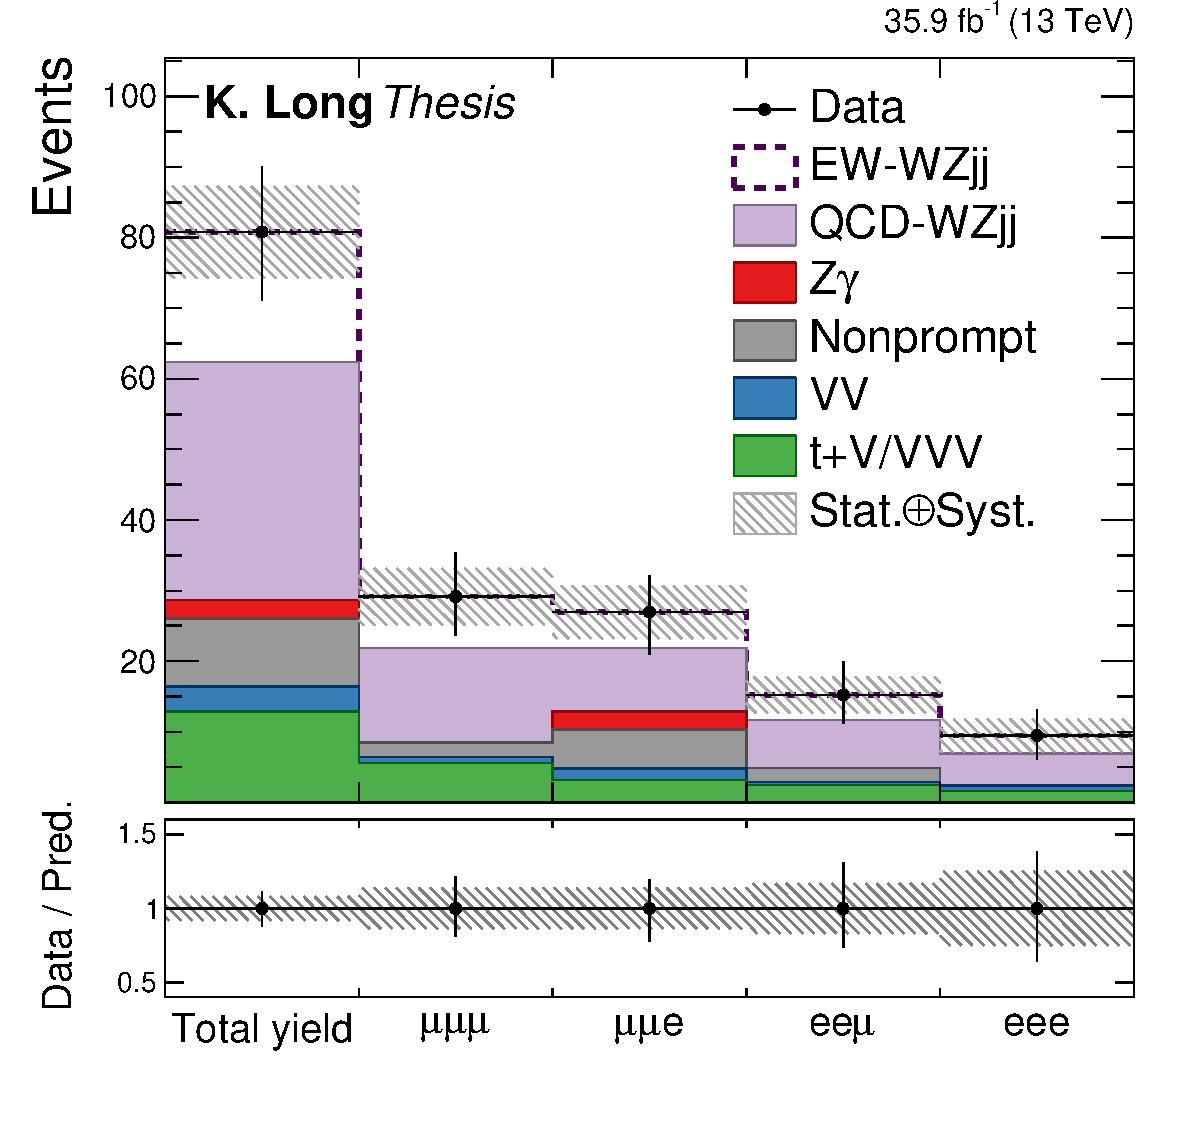
\includegraphics[width=0.6\textwidth]{figures/AnalysisProcedure/expectedYield_EWSignal.pdf}
  \caption[Expected composition of signal and background events for the EW signal selection]{
    Expected composition of signal and background events for the EW signal selection.
    The expected sum of signal and background contributions are treated as the observed
    data in a maximum likelihood fit. The uncertainty in the total expected event yield
    from WZ and non-WZ contributions is shown as a hashed band.
        }
 \label{fig:expectedEWSignal}
\end{figure}

The observed cross section is obtained from the value of $\mu_{\WZjj}$ 
which maximizes the likelihood function given

\begin{equation}
  \sigma_{\WZjj , obs} = \mu_{EW}\times\sigma_{th} \,.
  \label{eq:sigmaObs}
\end{equation}

Note that this expression does not imply that $\sigma_{\WZjj, obs}$
depends directly on the predicted cross section, as $\mu_{\WZjj}$ will adjust
linearly to fit the observed data, as seen in Equation~\ref{eq:wzjjLikelihood}.
Thus any input value for $\sigma_{th}$ will lead to the same $\sigma_{\WZjj , obs}$
given by Equation~\ref{eq:sigmaObs}, provided the efficiency for
reconstructing the events is unaffected. In terms of the efficiency for reconstruction
$\epsilon$, which is given by the ratio of expected events in the fiducial
volume to the number of reconstructed events,  $\epsilon = n_{th}/n_{reco}$.

In this expression, the number of expected events $n_{th}$ excludes events
outside the fiducial volume of the detector, or outside the kinematic region
where events can reasonably be reconstructed, e.g., leptons at very low \pt.
For this reason, the cross section obtained from this expression is referred to 
as a fiducial cross section.
To report a cross section in a region that difference significantly from the 
experimental fiducial volume, the extrapolation factor from the region
of measurement must be calculated. This fully theoretical quantity, known
as the acceptance, introduces a theoretical uncertainty to the measurement.
It is defined as $\mathcal{A} = \sigma_{report, th}/\sigma_{meas, th}$ where
$\sigma_{meas, th}$ and $\sigma_{report, th}$ are the predicted cross sections
in the region of measurement and reported region respectively. The fiducial
cross section regions considered in this analysis are described in Section~\ref{sec:eventselection}.

\subsection{Search for \EWWZ boson production}
\label{sec:EWWZ}

Separating the EW- and QCD-induced components of \WZjj events requires exploiting the different 
kinematic signatures of the two processes.
The relative fraction of the \EWWZ process with respect to the \QCDWZ process and other backgrounds
grows with increasing values of the $\mjj$ and $\left|\etajj\right|$
the leading jets, as demonstrated in Fig.~\ref{fig:VBSPlotsExpected},
which shows the expected distributions of $\mjj$ and $\etajj$ for events satisfying the EW signal selection.
This motivates the use of a 2D distribution built from these variables for the extraction of the EW \WZjj
signal strength via a maximum likelihood fit.
This 2D distribution, 
shown as a one-dimensional histogram in Fig.~\ref{fig:2DfitDistributionExp},
along with the yield in the control region defined in 
Section~\ref{sec:eventselection}, are combined in a binned likelihood
involving the expected and observed numbers of events in each bin.
The distribution including the yield in the \QCDWZ control region, shown as the first bin,
is shown in Fig.~\ref{fig:2DfitDistributionExpWCR}.

\begin{figure}[htbp]
  \centering
   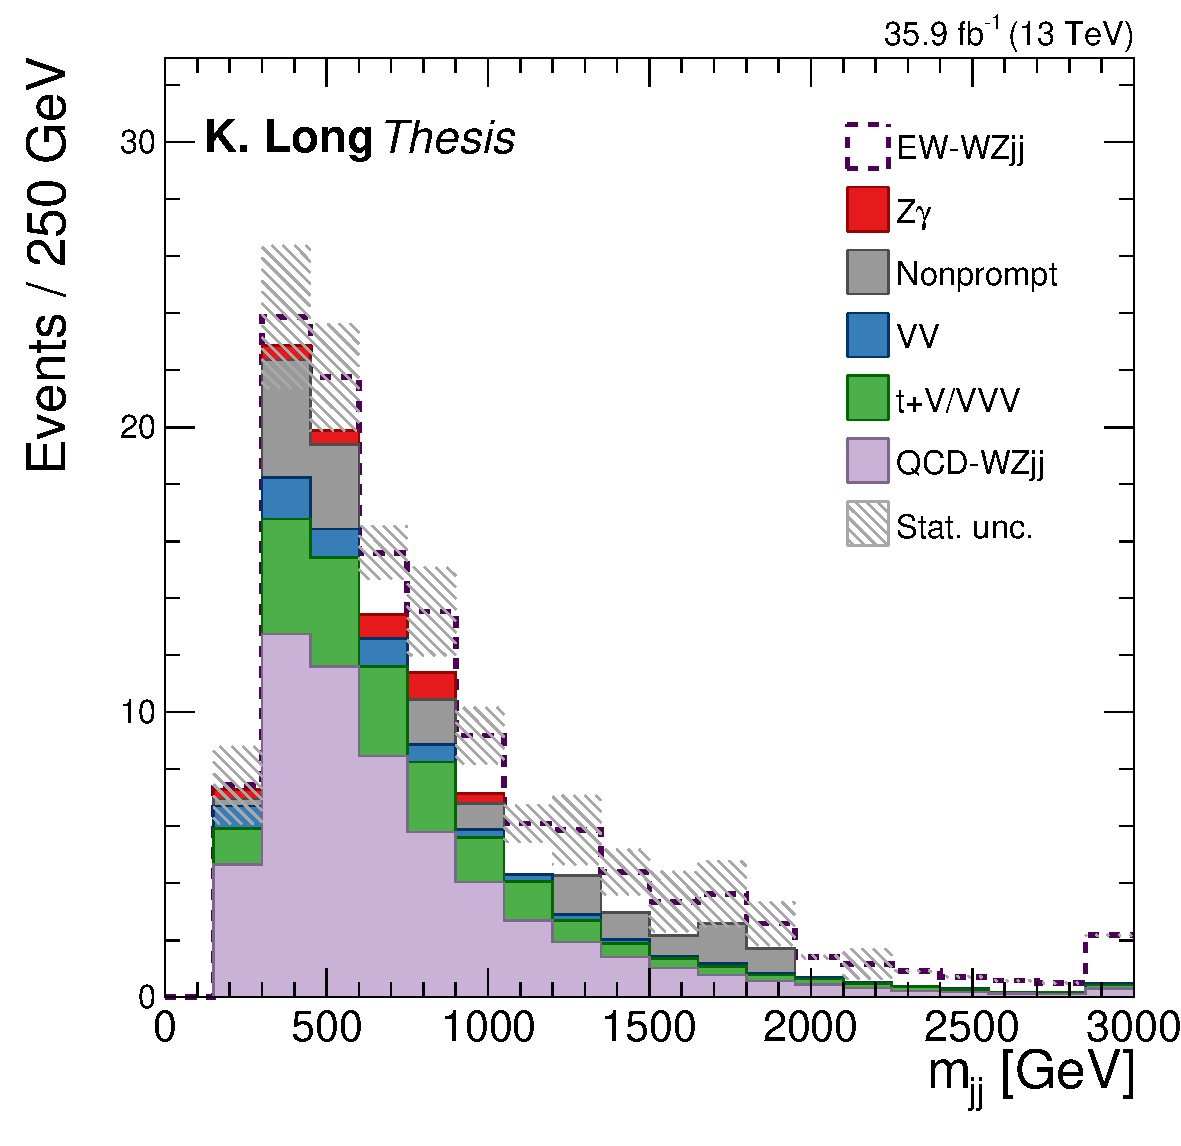
\includegraphics[width=0.45\textwidth]{figures/AnalysisProcedure/mjj_nMinus1.pdf}
   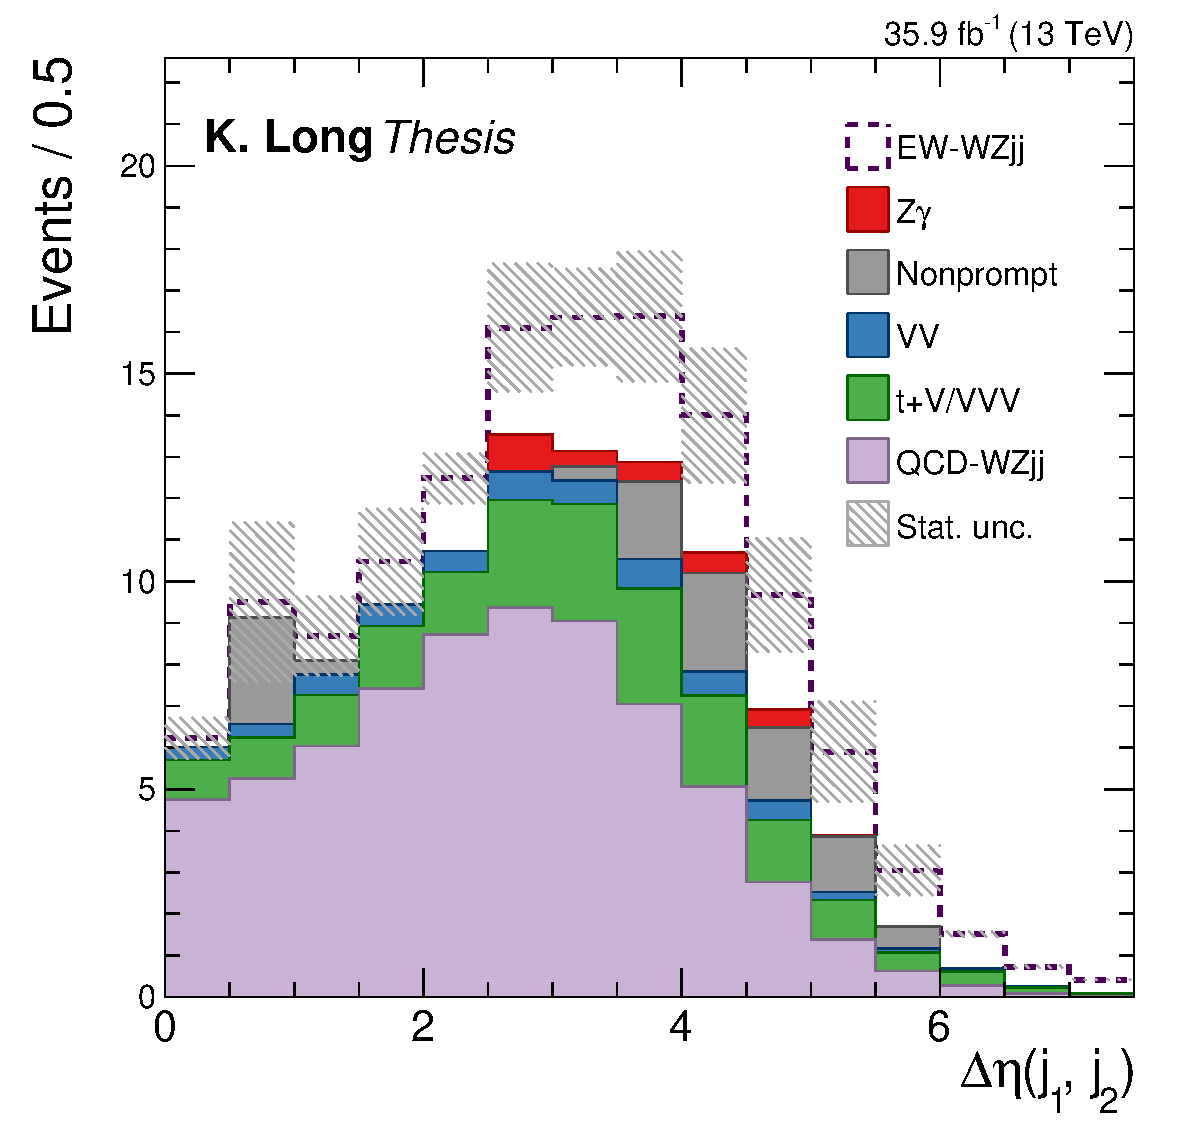
\includegraphics[width=0.45\textwidth]{figures/AnalysisProcedure/dEtajj_nMinus1.pdf}
  \caption[The $\mjj$ (left) and $\left|\etajj\right|$ of the two leading jets 
  (right) for events satisfying the EW signal selection]{
  The $\mjj$ (left) and $\left|\etajj\right|$ 
  of the two leading jets 
  (right) for events satisfying the EW signal selection. 
  The last bin contains all events with $\mjj > 2500\GeV$ (left) and 
  $\left|\etajj\right| > 7.5$ (right).
  The dashed line shows the expected \EWWZ contribution stacked
  on top of the backgrounds, which are shown as filled histograms. 
  The hatched bands represent the total and relative 
  statistical uncertainties on the predicted yields.
  The bottom panel shows the ratio of the number of events measured in data to the total 
  number of expected events. 
  The predicted yields are shown with their pre-fit normalizations.
          }
 \label{fig:VBSPlotsExpected}
\end{figure}
\begin{figure}[htbp]
  \centering
   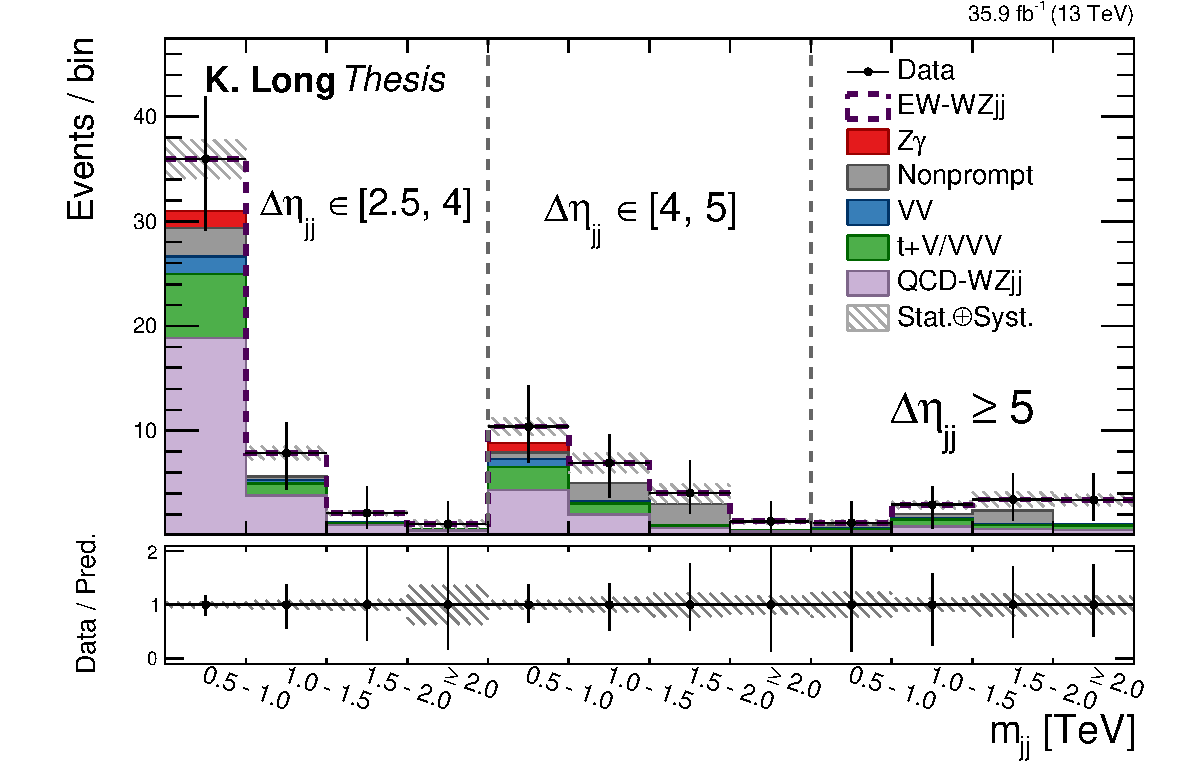
\includegraphics[width=0.7\textwidth]{figures/AnalysisProcedure/mjj_etajj_unrolled_Expected.pdf}\qquad
  \caption[The one-dimensional representation of the 2D distribution of 
    $\mjj$ and $\left|\etajj\right|$, used for the \EW signal region]{
    The one-dimensional representation of the 2D distribution of 
    $\mjj$ and $\left|\etajj\right|$, used for the EW 
    signal extraction. The x axis shows the dijet mass distribution
    in the indicated bins, split into three bins of {\etajj }: {\etajj} $\in [2.5, 4], [4, 5], \ge 5$.
    The dashed line represents the \EWWZ contribution stacked
    on top of the backgrounds, which are shown as filled histograms. 
    The hatched bands represent the total and relative 
    systematic uncertainties on the predicted yields.
    The bottom panel shows the ratio of the number of events measured in data to the total 
    number of expected events. 
    The predicted yields are shown with their best-fit normalizations.
}
\label{fig:2DfitDistributionExp}
\end{figure}

\begin{figure}[htbp]
  \centering
   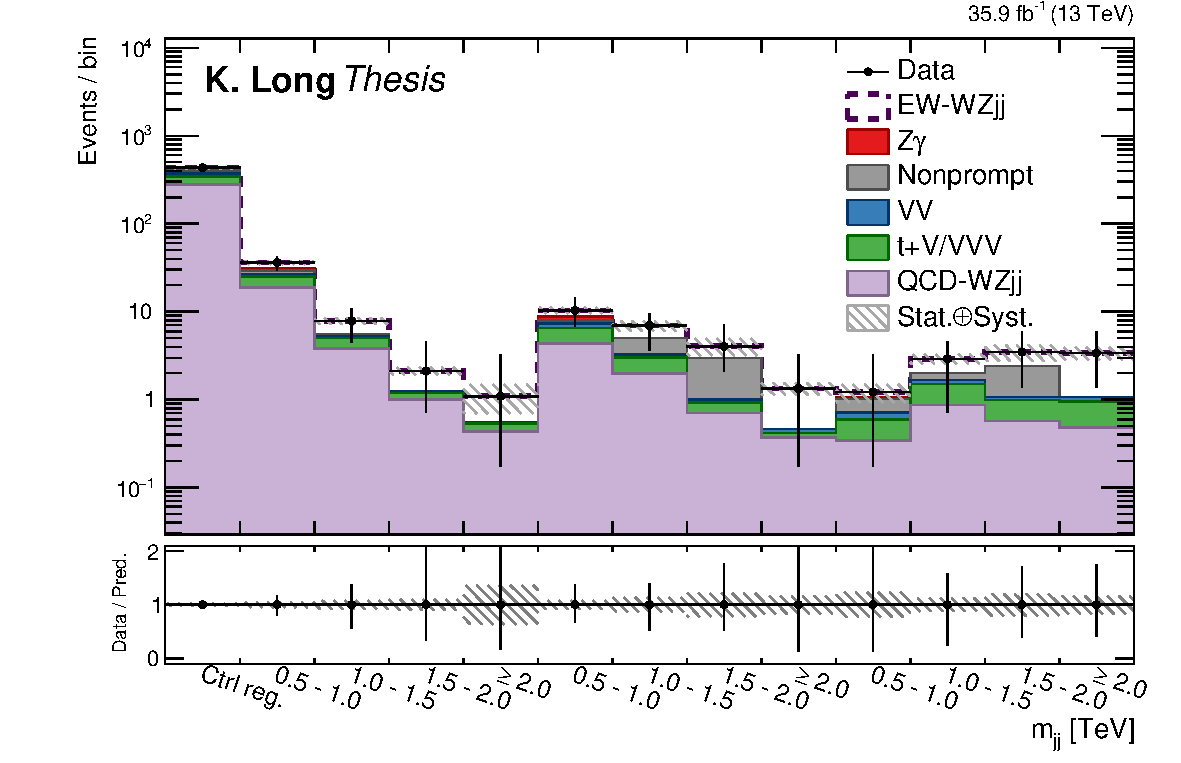
\includegraphics[width=0.7\textwidth]{figures/AnalysisProcedure/mjj_etajj_unrolled_wCR_Expected.pdf}\qquad
  \caption[Visualization of the likelihood function used for the \EWWZ search]{
    Visualization of the likelihood function used for the \EWWZ search.
    The first bin represents the yield in the low-\mjj control region,
    with other bins showing the one-dimensional representation of
    2D distribution of 
    $\mjj$ and $\left|\etajj\right|$ shown in~\ref{fig:2DfitDistributionExp}.
}
\label{fig:2DfitDistributionExpWCR}
\end{figure}

The likelihood is a combination of individual likelihoods for the four decay channels, 
following the definition of Equation~\ref{eq:likelihood}.
The measurement seeks to compare the best-fit value of $\mu_{\rm EW}$ from the 
maximum likelihood, to the background-only fit in which $\mu_{\rm EW} = 0$.
The significance of $\mu_{\rm EW}$ is a measure of the compatibility of the measurement
with the best-fit value of $\mu_{\rm EW} > 0$ obtained from the maximum likelihood
fit, referred to as the signal hypothesis, to
the background-only hypothesis. 

The compatibility of the measurement with the background-only hypothesises
is quantified via the test statistic, $t_{\mu}$, which is a function
of the best-fit signal strength and the model with $\mu = 0$. It is defined as

\begin{equation}
  t_{\mu} = \left\{ 
\begin{array}{c l}
  \frac{\mathcal{L}(\mu,{\bf \hat{\hat{\theta}}}(\mu))}
    {\mathcal{L}(\hat{\mu},{\bf \hat{\theta}})}           & \mu \ge \hat{\mu} \\
  \frac{\mathcal{L}(\mu,{\bf \hat{\hat{\theta}}}(\mu))}
    {\mathcal{L}(0,{\bf \hat{\theta}})}           & \mu < 0 \\

\end{array}\right\} \,,
\end{equation}

where $\hat{\mu}$ and ${\bf \hat{\hat{\theta}}}$ are the values of 
$\mu$ and ${\bf \hat{\theta}}$ which maximize the likelihood, and
${\bf \hat{\hat{\theta}}}(\nu)$ are the values of $\vec{\theta}$ which 
maximize the likelihood for the given $\mu$.
The significance of a measured value $\hat{\mu} \ne 0$ is quantified
via the test statistic $q_{0} = t_{\mu}(\mu = 0)$.
Note that the consistency with the background-only hypothesis is evaluated
with respect to the signal plus background hypothesis, and only a positive
signal strength is considered a signal-like deviation from the background.

The test statistic has a probability distribution $f(q_{\mu} | \mu)$
for a given $\mu$. This distribution can be determined by sampling the underlying
model and nuisance parameters to form an ensemble of pseudo-experiments drawn
from a value of $\mu$. The observed value $\hat{\mu}$ obtained from a fit 
to the data corresponds to a single realisation of the possible observations
given the underlying model. 
As sampling of the distribution is extremely computationally extensive,
it is common for particle physics results to be derived with asymptotic
formulae to approximate the distribution of $f(q_{\mu} | \mu)$ following Ref.~\cite{Cowan:2010js}.
These formulae are applicable provided the observed number of events 
per bin in the likelihood is not small. All results in this thesis 
use the asymptotic approach.

The probability of this result given the expected
parameters of the model in the background-only hypothesis
is quantified in terms of the $p$-value,

\begin{equation}
  p_{\mu} = \int_{t_{\mu, obs}}^{\infty} f(t_{\mu} | \mu) {\rm d}t \,.
  \label{eq:pvalue}
\end{equation}

The value of $p_{0}$ (or $p$-value) is customarily transposed such that the area from
$x=\pm\sigma$ to $x=\pm\infty$ for a Gaussian function with unit area and standard
deviation $\sigma$ would give the same value. This value, in terms of the standard
deviation, is referred to as the significance of the result.
It is customary in the particle physics community to refer to a $p$-value
of $2.87 \times 10^{-7}$, corresponding to a significance of 5 standard 
deviations, or $5 \sigma$, as sufficient for rejection of the background-only
hypothesis in favor of the signal plus background model. 

The expected significance of \EWWZ process obtained from a fit to the likelihood
shown in Fig.~\ref{fig:2DfitDistributionExpWCR},
based on the expected distribution
of background and signal events with $\mu_{\mathrm{EW}} = 1$, is 2.5 standard deviations.

\subsection{Limits on charged Higgs boson production}

For the \EWWZ search, the background-only assumption corresponds to the SM with
no \EWWZ process. An excess with respect to the background-only hypothesis is therefore
expected, and is quantified using the procedures of the previous section. For searches 
for BSM physics, one does not anticipate the need to quantify the significance of a signal-like
fluctuation. One seeks instead to place constraints on the parameters of the unobserved BSM model
based on the consistency of the search with the null hypothesis. 

Upper limits on the signal strength is are derived using the CL$_{s}$ criterion of Refs.~\cite{Junk:1999kv,CLS2,Cowan:2010js}.
The procedure follows the approach of the previous section, with a
slight modification of the test statistic,
defined as

\begin{equation}
  t_{\mu} = \left\{ 
\begin{array}{c l}
  \frac{\mathcal{L}(\mu,{\bf \hat{\hat{\theta}}}(\mu))}
    {\mathcal{L}(\hat{\mu},{\bf \hat{\theta}})}           & \mu \ge \hat{\mu} \\
  \frac{\mathcal{L}(\mu,{\bf \hat{\hat{\theta}}}(\mu))}
    {\mathcal{L}(0,{\bf \hat{\theta}})}           & \mu < \hat{\mu} \\

\end{array}\right\} \,.
\end{equation}


The distribution of expected results and the 
$p$-value of the observation are calculated from this test statistic for a 
range of possible values of $\mu$ for the signal hypothesis using
Equation~\ref{eq:pvalue}. The CL$_{s}$ criterion is defined as

\begin{equation}
  \mathrm{CL}_{s} = \frac{p_{\mu}}{p_{0}} \,.
\end{equation}

The signal strength $\mu$ that satisfies the condition
${\rm CL}_{s} = 1 - \alpha$ is said to be excluded at 
confidence level (CL) $\alpha$. For example, the value $\alpha=0.95$ corresponds
to an exclusion limit of 95\% CL.

Because presence of charged Higgs bosons would give rise to a resonance-like structure in the 
\WZ transverse mass, defined as

\begin{equation}
  \mt = \sqrt{(\ET(\W) + \ET(\Z))^2 - (\vec{\PT}(\W) + \vec{\PT}(\Z))^2} \, ,
  \label{eq:wztransmass}
\end{equation}

with $\ET = \sqrt{m^2 + \PT^2}$,
where the \W candidate is constructed from 
the \ptvecmiss 
and the lepton associated with the $\PW$ boson,
the likelihood used to test the consistency of the data with the presence of a charged Higgs
boson is built from this distribution, shown in Fig.~\ref{fig:higgsmtExp}, 
and the event yield in the
control region described in Section~\ref{sec:promptbackgrounds}.
A combined fit of the predicted signal and background yields to the data 
in the Higgs boson selection is performed 
to derive model-independent expected and observed upper limits on $\sigma_\mathrm{VBF}(\PHpm) \, 
\mathcal{B}(\PHpm\to \PW\Z)$ at 95\% CL using the CL$\mathrm{_s}$ criterion. 

\begin{figure}[htbp]
  \centering
    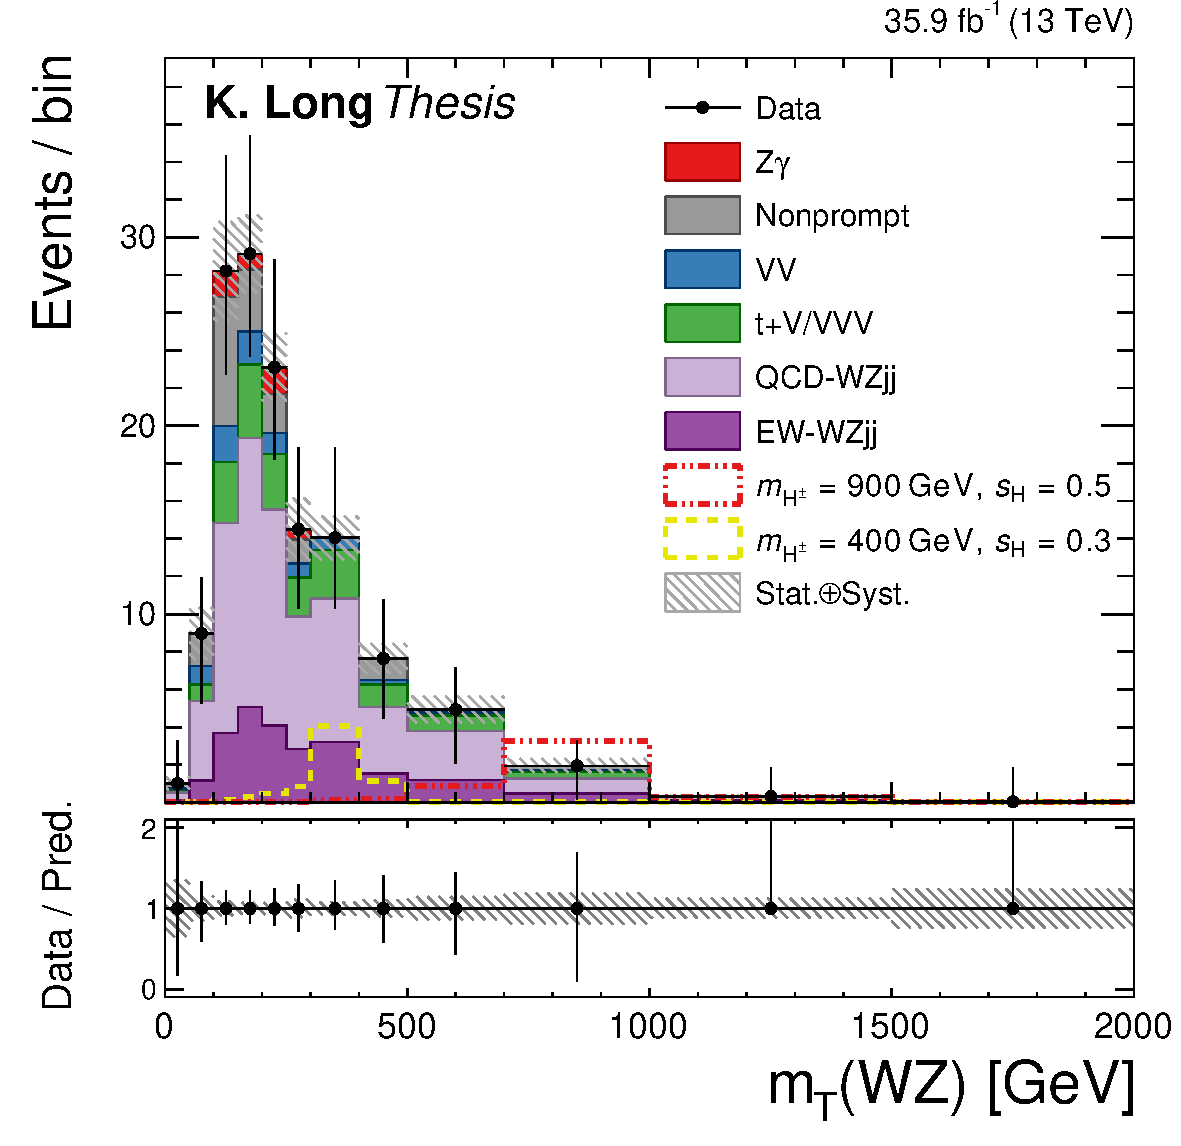
\includegraphics[width=0.6\textwidth]{figures/AnalysisProcedure/MTWZ_Higgs_expected.pdf}
  \caption[The $\mt$ for events satisfying the Higgs boson selection]{
      The $\mt$ for events satisfying the Higgs boson selection,
      used to place constraints on the production of charged Higgs bosons.
      The last bin contains all events with $\mt > 2000\GeV$.
      The dashed lines show predictions from the Georgi-Machechek model with
      $m(\PHpm) = 500 \,(900)\GeV$ and $s_{\PH} = 0.3 \,(0.5)$.
      The bottom panel shows the ratio of the number of events measured in data to the total 
      number of expected events. The hatched bands represent the total and relative 
      systematic uncertainties on the predicted background yields.
      The predicted yields are shown with their best-fit normalizations from the background-only fit.
      }
 \label{fig:higgsmtExp}
\end{figure}

\subsection{Limits on anomalous quartic gauge couplings}
\label{sec:aqgcProcedure}

Events satisfying the EW signal selection are used to constrain aQGCs in the effective field theory approach~\cite{Degrande:2012wf}.
Results are obtained following the formulation of Ref.~\cite{Eboli:2006wa}, which proposes
nine independent dimension-eight operators which assume the presence of a light Higgs boson and 
respect the {\SUtwo$\times$\Uone} symmetry of the EW gauge sector. All operators are
charge conjugation and parity-conserving.
The \WZjj channel is most sensitive to the 
T0, T1, and T2 operators, which are constructed purely from the {\SUtwo} gauge fields,
the S0 and S1 operators, which involve interactions with the Higgs field,
and the M0 and M1 operators, which involve a mixture of gauge and Higgs field interactions.

The presence of nonzero aQGCs would enhance the production of events with high 
WZ mass. The binned likelihood used for the extraction of results
is therefore built from $\mt$ as for the limits on charged Higgs bosons. The 
expected distribution is shown in Fig.~\ref{fig:aQGCDistributionExp}, 
with several illustrative anomalous coupling parameters also shown.

\begin{figure}[htbp]
  \centering
    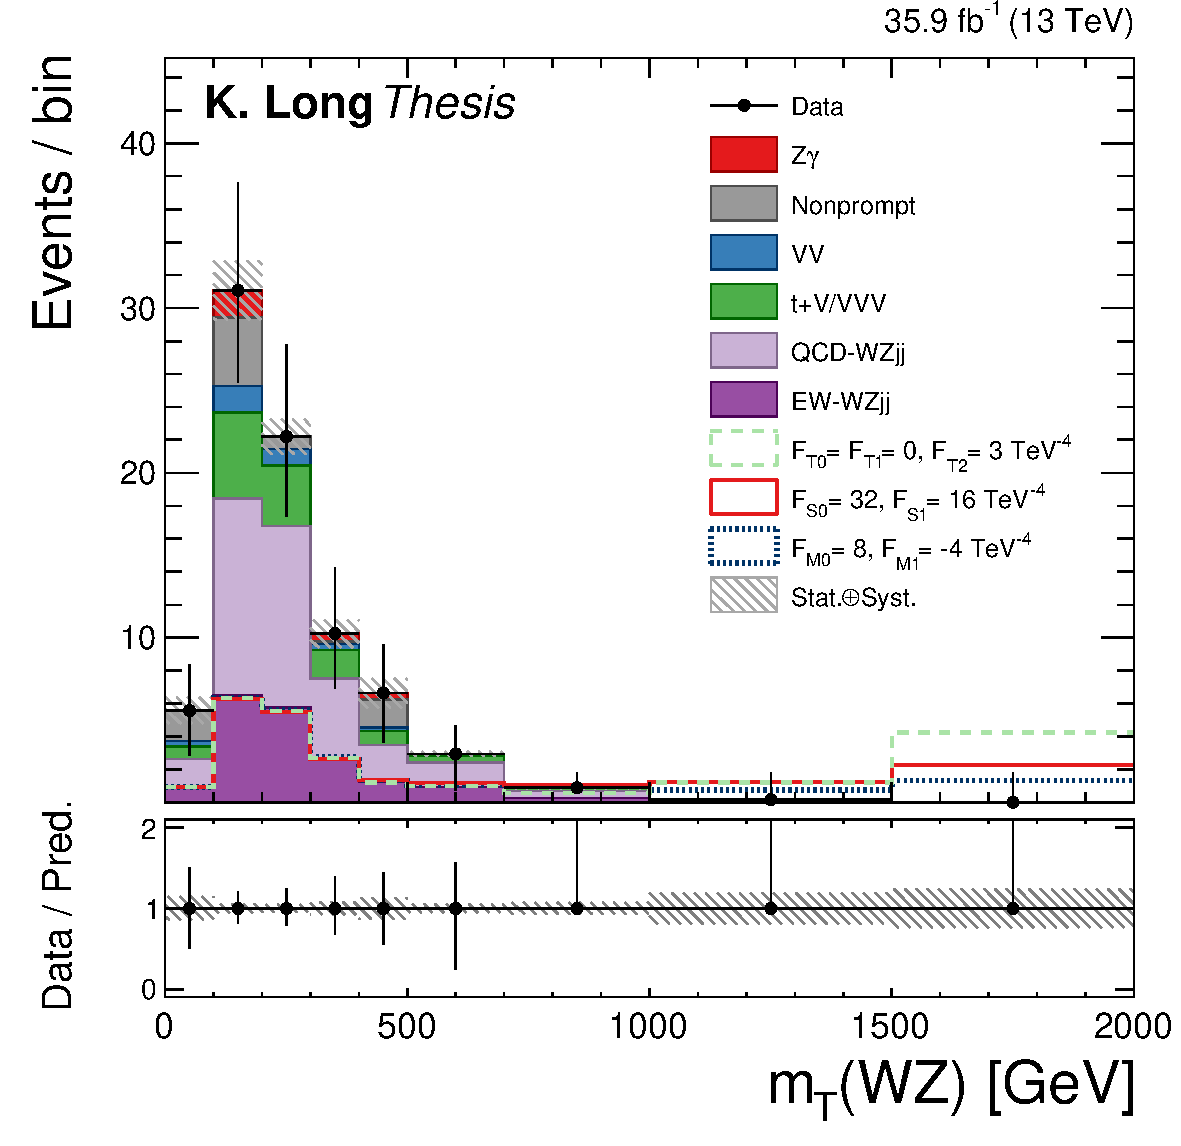
\includegraphics[width=0.6\textwidth]{figures/AnalysisProcedure/MTWZ_aQGC_expected.pdf}
  \caption[The $\mt$ for events satisfying the EW signal selection]{
      The $\mt$ for events satisfying the EW signal selection,
      used to place constraints on the anomalous coupling parameters.
      The dashed lines show predictions for several aQGC parameters values, which modify the \EWWZ process.
      The last bin contains all events with $\mt > 2000\GeV$.
      The hatched bands represent the total and relative 
      systematic uncertainties on the predicted yields.
      The bottom panel shows the ratio of the number of events measured in data to the total 
      number of expected events. 
      The predicted yields are shown with their best-fit normalizations from the background-only fit.
      }
 \label{fig:aQGCDistributionExp}
\end{figure}

The MC simulations of non-zero aQGCs include the SM \EWWZ process, with an increase
in the yield at high $\mt$ arising from parameters different from their SM values. 
Because the increase of the expected yield over the SM prediction exhibits a quadratic 
dependence on the operator coefficient, 
a parabolic function is fitted to the predicted yields per bin to obtain a smooth interpolation
between the discrete operator coefficients considered in the MC simulation.
The one-dimensional 95\% CL limits are extracted 
using the CL$\mathrm{_s}$ criterion
as for the charged Higgs boson search.
The SM prediction, including the \EWWZ process, is treated as the null hypothesis.

One-dimensional limits are placed with all
parameters except for the coefficient being probed set to zero.
In addition, a scan of the likelihood is also performed with multiple independent
$\mu$ values corresponding to different dimension-eight operators. 

Constraints are also placed on aQGC parameters using a two-dimensional scan,
where two parameters are probed in the fit with all others set to zero.
In this case, the likelihood is a function of two signal strength parameters,
and a two-dimensional exclusion region is defined by the region
in $\mu_1$ and $\mu_2$ space in which the likelihood differs
from its maximum value by the desired confidence interval.

\section{Systematic uncertainties}
\label{sec:systematics}

The dominant uncertainties in both the cross section measurement 
and new physics searches are those associated with 
the jet energy scale (JES) and resolution (JER).  The JES and JER 
uncertainties are applied in simulated events by smearing and 
scaling the relevant
observables and propagating the effects to the event selection and 
the kinematic variables used in the analysis.
The uncertainty in the event yield in the EW signal selection
due to the JES and JER 
is found to be 9\% for \QCDWZ and 5\% for \EWWZ processes.
The uncertainty additionally depends on the $\pt$ and $\eta$ of the selected
jets. For the \QCDWZ process, it varies in the range of 5--25\% with
increasing values of {\mjj} and $\left|\etajj\right|$.

Uncertainties in signal and background processes estimated with
MC simulation are evaluated from the theoretical uncertainties 
of the predictions. 
Event weights in the simulated samples are used to evaluate 
variations of the central prediction.
Scale uncertainties are estimated by varying
$\mu_{\mathrm{R}}$ and $\mu_{\mathrm{F}}$ by a factor of two from their
nominal values, with the condition that $1/2 \le \mu_{\mathrm{R}}/\mu_{\mathrm{F}} \le 2$.
The maximal and minimal variations are obtained
per bin to form a shape-dependent variation band.
The PDF uncertainties are obtained from the MC replica sets 
of the NNPDF3.0 PDF. 
The PDF and scale uncertainties are uncorrelated for different signal and
background process and 100\% correlated across bins for the distributions
used to extract results.

\begin{figure}
\centering
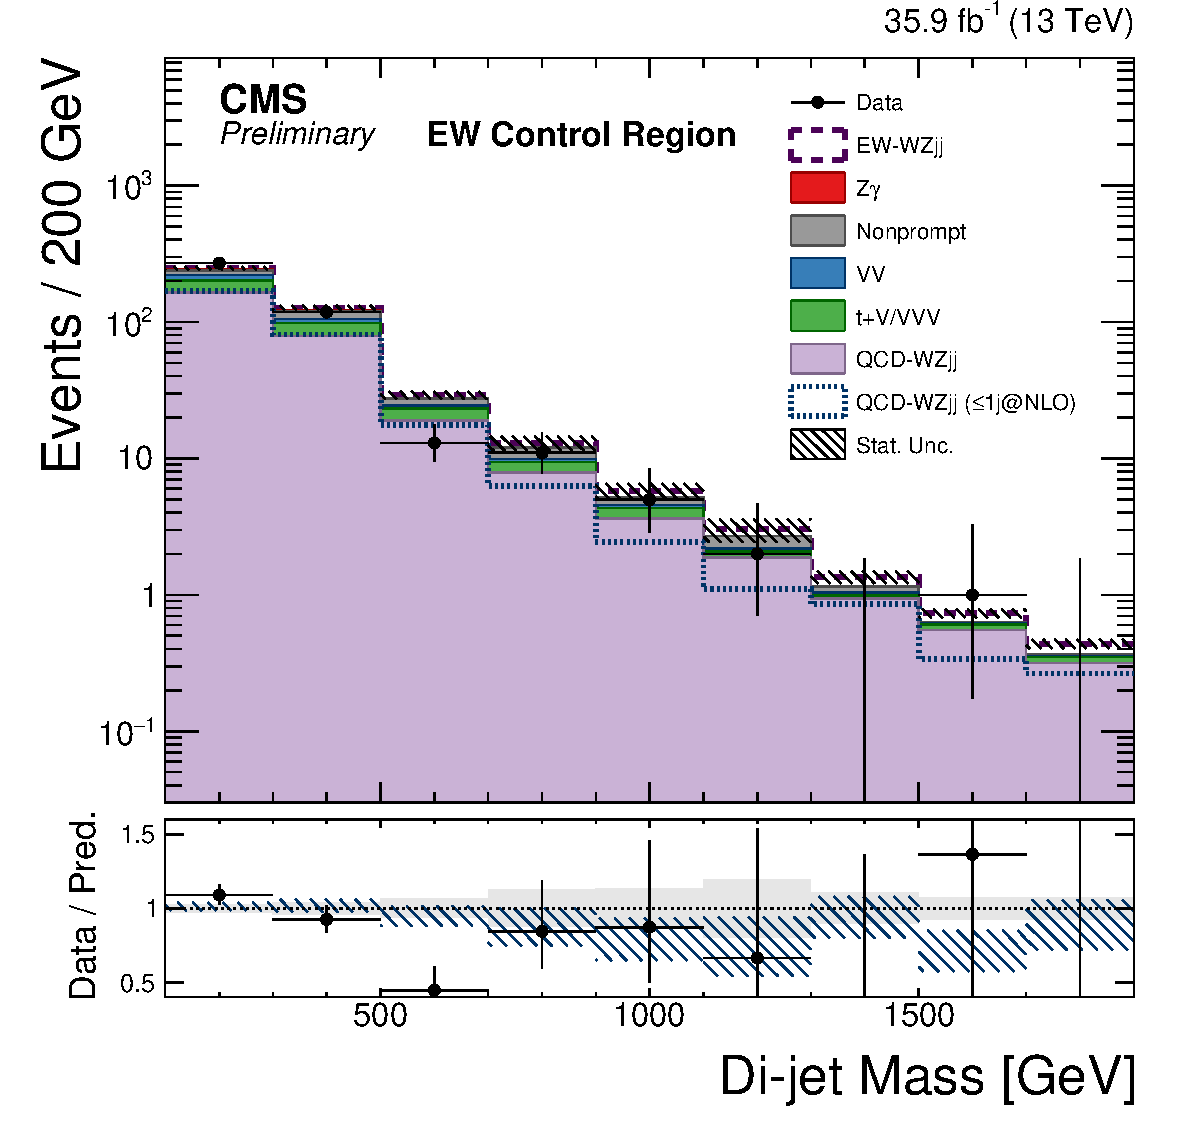
\includegraphics[width=0.45\textwidth]{figures/AnalysisProcedure/mjj_backgroundControl.pdf}
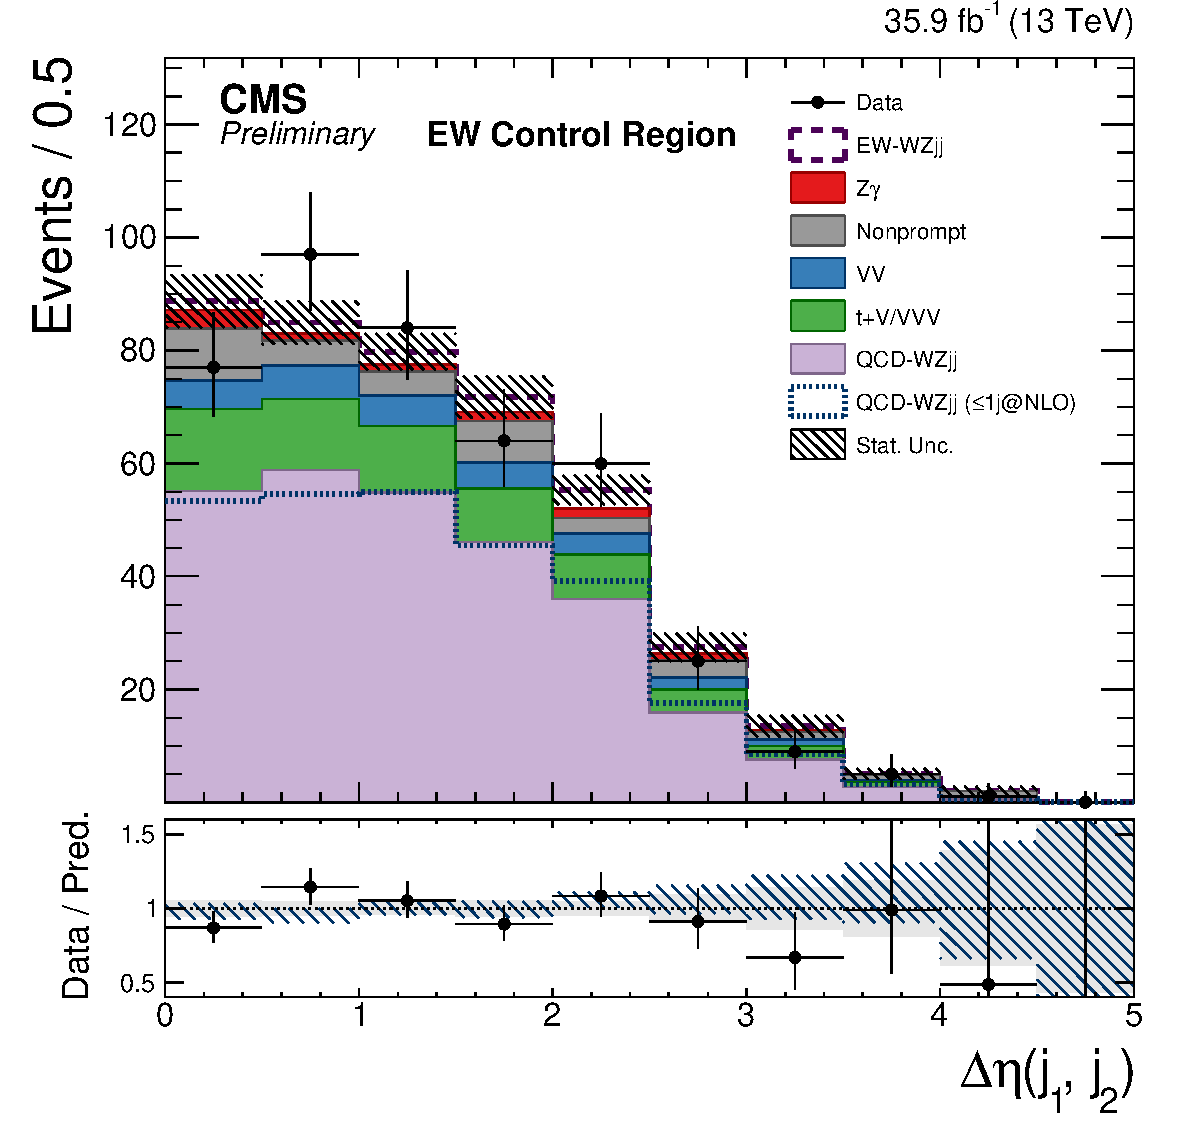
\includegraphics[width=0.45\textwidth]{figures/AnalysisProcedure/dEtajj_backgroundControl.pdf}
  \caption[The $\mjj$ (left) and $\etajj$ (right) for events in the non-VBS control region]{
  The $\mjj$ (left) and $\etajj$ (right) for events in the non-VBS control region. 
  The last bin contains all events with $\mjj > 1900\GeV$ (left) and 
  $\left|\etajj\right| > 5.0$ (right).
  An alternative prediction for the 
  QCD WZ contribution, using \MG with FxFx merging as described in the text of SMP-18-001, 
  is shown in dashed blue. This distribution can be compared to the nominal prediction 
  in filled purple. The bottom panel shows the ratio of the number of events measured 
  in data to the total number of expected events for the nominal QCD WZ prediction. 
  The shaded band at 1 represents the size of the statistical uncertainties on the 
  predicted yields. The hatched blue band shows the sum of Monte Carlo 
  predictions and statistical uncertainties with the alternative QCD WZ prediction 
  divided by the sum of Monte Carlo predictions with the nominal QCD WZ prediction. 
  Normalizations are shown as values used for the input to the fit.
}
  \label{fig:backgroundControl}
\end{figure}

The uncertainty in modeling the \EWWZ and \QCDWZ
processes has a large impact in the \EWWZ measurement.
In addition to the uncertainties from scale and PDF choice,
comparisons of alternative matrix element and parton shower generators are
considered.
The uncertainty in the \QCDWZ process is derived by
comparing the predictions of the MLM-merged simulation and those obtained with the \FxFx-merged simulation,
after fixing the normalization to the observed data
in the \QCDWZ sideband region.
Differences between the predictions of the MC simulations
in the signal region and in the ratio
of the \QCDWZ sideband to the signal region event yields
are considered in the comparisons.
The differences in predictions are generally
within the scale and PDF uncertainties of the MC simulations,
and a 10\% normalization uncertainty is assigned to account for
the observed discrepancies.
The results obtained using the \POWHEG simulation,
which predicts a slightly softer {\mjj} spectrum, are also largely contained
within the theoretical uncertainties considered.
However, because \WZjj events from this simulation arise from
soft radiation from the parton shower, it is
not explicitly considered in the uncertainty evaluation.
For the \EWWZ process, the MC simulations described in Section~\ref{sec:promptbackgrounds}
agree within
the theoretical uncertainties from the PDF and the choice of
$\muR$ and $\muF$
for the kinematic variables considered in the analysis,
so no additional uncertainty is
assigned.

The interference term is evaluated using MC simulation of particle-level events
selected from the samples described in Section~\ref{sec:promptbackgrounds}. 
It is found to be positive, and amounts to 12\% 
of the \EWWZ contribution in the control region and 4\% in the signal region
for both MC samples considered. 
The ratio of the interference to the \EWWZ 
decreases with increasing $\mjj$, consistent with the observations of Ref.~\cite{leshouches2017}.
These values are used as a symmetric shape uncertainty in the 
signal cross section when performing the 
\EWWZ measurement.
This uncertainty is subdominant with respect to other theoretical uncertainties 
and has a negligible contribution to the uncertainty 
on the observed \EWWZ signal strength.

Higher-order EW corrections in VBS processes are known to be negative and at
the level of tens of percent, with the correction increasing in magnitude 
with increasing {\mjj}~\cite{Biedermann:2016yds} and $m_{\mathrm{VV}}$.
We do not apply corrections to the \WZjj MC simulation, but we have verified that the 
significance of the \EWWZ measurement is insensitive to higher-order EW corrections by 
performing the signal extraction described in Section~\ref{sec:EWWZ} with the \mjj predicted 
by the \EWWZ MC simulation modified by the corrections from Ref.~\cite{Denner:2019tmn}. 
As the relative effect of the EW corrections on SM and anomalous \WZjj production is unknown, 
we do not apply corrections to the SM backgrounds or new physics signals for our results. 
Because corrections to the SM \WZjj production that decrease the expected number of events 
at high $m_{\WZ}$ lead to more stringent limits on new physics, this is a conservative approach.

The uncertainties related to the finite number of simulated events, or to the limited
number of events in data control regions, affect the signal and background predictions.
They are uncorrelated
across different samples, and across bins of a single distribution.
The limited number of events in the relaxed lepton control samples used for the
nonprompt background estimate is the dominant contribution to this uncertainty.

The nonprompt background estimate is also affected by systematic uncertainties
from the jet flavor composition of the control regions and loose-to-tight transfer factors.
The systematic uncertainty in the nonprompt event yield is 30\%
for both electrons and muons, uncorrelated between channels.
It covers the largest difference observed
between the estimated and measured
numbers of events in data control samples enriched in
$\ttbar$ contributions, which have enhanced contributions from heavy-flavor jets, and
Drell--Yan contributions, dominated by light-flavor jets, and the differences between 
using transfer factors derived in \Zpj and dijet events.

Systematic uncertainties are less than 1\% for the trigger efficiency and 1--3\% for the
lepton identification and isolation requirements, depending on the lepton flavors.
Other systematic uncertainties are related to the use of simulated samples:
1\% for the effects of pileup and  1--2\% for the \ETmiss reconstruction,
which is estimated by varying the energies of the PF objects within their uncertainties.
The uncertainty in the b-quark jet content in $\PW\PZ$ events is 2\%
and accounts for differences in b-tagging efficiencies between data and MC.
The uncertainty in the integrated luminosity of the data sample is 2.5\%~\cite{CMS:2017sdi}.
This uncertainty affects both the signal and the simulated portion of the background estimation,
but does not affect the background estimation from data.

\begin{table}[htbp]
     \centering
     \caption[The dominant uncertainty contributions in the fiducial \WZjj cross section measurement ]
     { The dominant uncertainty contributions in the fiducial 
         \WZjj cross section measurement 
         and their expected contributions to the significance of the
         \EWWZ measurement. The impact of each systematic 
         uncertainty in the \WZjj 
         cross section measurement is obtained by freezing the set of associated nuisance 
         parameters to their best fit values and comparing the total uncertainty in the signal strength
         to the result from the nominal fit. 
         The effect on the \EWWZ significance, shown in the last column,
         is defined as the relative increase in the expected significance when
         freezing the nuisance term to its best fit value.
           }
     \begin{tabular}{l|ccc}
 \hline %------------------------------------------------------------------------------------------
     Source of systematic uncertainty & \multicolumn{3}{c}{Relative systematic uncertainty [\%]} \\
                                      & $\sigma_{\WZjj}$ & \EWWZ significance \\
 \hline %------------------------------------------------------------------------------------------
 \hline %------------------------------------------------------------------------------------------
 Jet energy scale                     & $+11\, /-8.1$ & $ 7.0 $               \\ %done
 Jet energy resolution                & $+1.9\,/-2.1$   & $< 0.1$             \\ %done
 \QCDWZ modeling                      &    N/A          & $ 2.2 $             \\
 Other background theory              &  $+2.2\,/-2.2$  & $ 0.3 $             \\ %done
 Nonprompt normalization              &  $+2.5\,/-2.5$  & $ 0.3 $             \\ %done
 Nonprompt event count                &  $+6.0\,/-5.8$  & $ 1.7 $               \\ %done
 Lepton energy scale and eff.         &  $+3.5\,/-2.7$  & $< 0.1$             \\ %done
 b tagging                            &  $+2.0\,/-1.7$  & $< 0.1$             \\ %done
 Integrated luminosity                &  $+3.6\,/-3.0$  & $< 0.1$             \\ %done
 \hline %------------------------------------------------------------------------------------------
      \end{tabular}
     \label{tab:systematics}
\end{table}

